\documentclass[12pt,a4paper,twoside]{book}

\usepackage[ngerman,english]{babel}\selectlanguage{english}
\usepackage{booktabs}
\usepackage{calc}
\usepackage{colortbl}
\usepackage{fancyhdr} % chapternames at top of page
\usepackage{float}
\usepackage[T1]{fontenc}
\usepackage{glossaries}
\usepackage{graphicx}
\usepackage{ifpdf}
\usepackage[utf8]{inputenc} % for a UTF8 editor only
\usepackage{longtable}
\usepackage{newunicodechar}
\usepackage{pifont}
\usepackage{makeidx} % allows for an index
\usepackage{mathptmx} % font times-roman for math. Formulas, bullets, etc.
\usepackage{multicol}
\usepackage{multirow}
\usepackage{rotating}
\usepackage{sectsty}
\usepackage{siunitx}
\usepackage{subcaption} %to have subfigures available
\usepackage{threeparttable}
\usepackage[hyphens]{url}
\usepackage[svgnames,table,usenames,dvipsnames]{xcolor}

%\usepackage[top=2cm, bottom=1.25in, left=2cm, right=2cm]{geometry}
%\usepackage{enumitem}

%%%%%%%%%%%%%%%%%%%%%%%%%%%%%%%%
\usepackage{afterpage}
\usepackage{amsfonts}
\usepackage{amsmath}
\usepackage{amssymb}% http://ctan.org/pkg/amssymb
\usepackage{array}
%\usepackage{blindtext}
%\usepackage{caption}
\usepackage{csquotes}
\usepackage{csvsimple}
\usepackage[shortlabels]{enumitem}
\usepackage[gen]{eurosym}
%\usepackage[hang,splitrule]{footmisc} % avoid hanging footnotes
\usepackage{geometry}
\usepackage{ifthen} % allow sophisticated control structures
%\usepackage{marvosym}
\usepackage{mdframed}
%\usepackage[sort]{natbib}
\usepackage{nccfoots}
\usepackage{subscript}
\usepackage{substr} % allows substring detection
\usepackage{tabularx}
\usepackage{titlesec}
\usepackage[nottoc,notindex]{tocbibind} % include bib in toc
\usepackage[subfigure]{tocloft}
\usepackage{wrapfig}
%\usepackage[usenames,dvipsnames]{xcolor}

%TIKZ
%\usepackage{pgfplots}
%\pgfplotsset{compat=1.3}
%\usepackage{tikz}
%\usetikzlibrary{arrows, decorations.pathmorphing, decorations.markings, backgrounds, positioning, fit, petri}


\newcolumntype{L}[1]{>{\raggedright\arraybackslash}p{#1}} % linksbündig mit Breitenangabe
\newcolumntype{C}[1]{>{\centering\arraybackslash}p{#1}} % zentriert mit Breitenangabe
\newcolumntype{R}[1]{>{\raggedleft\arraybackslash}p{#1}} % rechtsbündig mit Breitenangabe


\definecolor{platinum}{HTML}{E5E4E2}
\colorlet{diagrambg}{platinum}

\makeindex

\geometry{a4paper,twoside,inner=97pt,outer=110pt,top=118pt,textheight=592pt,marginpar=68pt,marginparsep=2pt,bindingoffset=8mm} % for some weird reason oddsidemargin is originally -108pt


\newcommand{\mytitle}{Supporting Users in Password Authentication with Persuasive Design}
\newcommand{\mysubtitle}{}
\newcommand{\myname}{Tobias Seitz}
\newcommand{\ie}{i.e.,\ }
\newcommand{\eg}{e.g.,\ }


\definecolor{pinkaccent}{HTML}{F50057}
\definecolor{darkindigo}{HTML}{303F9F}
\definecolor{lightblue}{HTML}{c5cae9}
\definecolor{primaryblue}{HTML}{3f51b5}
\definecolor{verylightblue}{HTML}{B5BDEA}
\definecolor{bluegray}{HTML}{607d8b}
\definecolor{secondarygray}{HTML}{757575}
\definecolor{dividergray}{HTML}{bdbdbd}
\definecolor{almostwhite}{HTML}{eaeaea}



%Stats
\newcommand{\statslt}[3]{\textit{F\textsubscript{#1}}~$=$~#2, \textit{p}~$<$~#3}
\newcommand{\stats}[3]{\textit{F\textsubscript{#1}}~$=$~#2, \textit{p}~$=$~#3}
\newcommand{\statsgt}[3]{\textit{F\textsubscript{#1}}~$=$~#2, \textit{p}~$>$~#3}
\newcommand{\pval}[1]{\textit{p}~$=$~#1}
\newcommand{\pvallt}[1]{\textit{p}~$<$~#1}
\newcommand{\pvalgt}[1]{\textit{p}~$>$~#1}
\newcommand{\mean}[2]{\textit{m}~$=$~#1, \textit{sd}~$=$~#2}
\newcommand{\meant}[2]{\textit{m}$=$#1 \textit{sd}$=$#2}
\newcommand{\meanonly}[1]{\textit{m}~$=$~#1}
\newcommand{\median}[1]{\textit{median}~$=$~#1}
\newcommand{\average}{average:\xspace}
\newcommand{\Rsqadj}[1]{$R_{adj}^2$~$=$~#1}
%tables and figures
\newcommand*{\thead}[1]{\multicolumn{1}{c}{\bfseries #1}}
\newunicodechar{✓}{\ding{51}}
\newunicodechar{✘}{\ding{56}}
\newunicodechar{↗}{\ding{246}}
\newunicodechar{↘}{\ding{244}}

% emojis
\newlength\myheight
\newlength\mydepth
\settototalheight\myheight{Xygp}
\settodepth\mydepth{Xygp}
\setlength\fboxsep{0pt}
\newcommand*\inlinegraphics[1]{%
	\settototalheight\myheight{Xygp}%
	\settodepth\mydepth{Xygp}%
	\raisebox{-\mydepth}{\includegraphics[height=\myheight]{#1}}%
}
\newcommand{\emoji}[2][ios]{\inlinegraphics{../latex-emoji/#1/#2}}%
% this works on a more rudimentary level: \newcommand{\emoji}[1]{\includegraphics[width=1em]{../latex-emoji/ios/#1}}%

\newcommand{\citep}[1]{\cite{#1}} %convenience for texmaker, but texstudio doesn't have this problem. % natbib package

\graphicspath{{figures/}}

%SHORTCUTS
\label{Shortcuts}
\usepackage{xspace}
\newcommand{\percent}{\%\xspace}
\newcommand{\seefig}{see Figure\xspace}
\newcommand{\red}[1]{\textcolor{red}{#1}}
\newcommand{\access}[1]{\textit{(last accessed #1)}}
\newcommand{\la}[1]{\textit{(last accessed #1)}}
\newcommand{\lastaccess}[1]{\textit{(last accessed #1)}}
\newcommand{\footurl}[2]{\footnote{\url{#1} \lastaccess{#2}}}
%alternative approach: try if time:
%\newcommand{\footurl}[2]{
%	\bibitem{#1}~, \url{http://en.wikipedia.org/wiki/Business_logic_layer}, #2.
%	\cite{#1}
%}


\newcommand{\etal}{et al.\xspace}
\newcommand{\todo}[1]{\textcolor{pinkaccent}{\textbf{@TODO} {#1}}}
\newcommand{\ar}{\textcolor{pinkaccent}{\textbf{@ref}}}
\newcommand{\vspc}{\vspace*{2cm}}

\usepackage[light]{roboto}  %% Option 'sfdefault' only if the base font of the document is to be sans serif

\renewcommand{\floatpagefraction}{.8}% this avoids putting larger images onto separate pages.

% Footnote style.
\makeatletter
\renewcommand{\@makefntext}[1]{%
	\setlength{\parindent}{0pt}%
	\begin{list}{}{\setlength{\labelwidth}{1em}%
			\setlength{\leftmargin}{\labelwidth}%
			\setlength{\labelsep}{3pt}%
			\setlength{\itemsep}{0pt}%
			\setlength{\parsep}{0pt}%
			\setlength{\topsep}{0pt}%
			%   \setlength{\rightmargin}{0.2\textwidth}%
			\footnotesize}%
		\item[\@makefnmark\hfil]#1%
	\end{list}%
}
\makeatother

%%% SARAH's original:

% TEST :: BEGIN ========
\clubpenalty=10000
\widowpenalty=10000
\displaywidowpenalty=10000
%\interlinepenalty=5000
% TEST :: END ==========

% Quotes
\label{Quotes}
\newcommand{\sciencequote}[3]{
	\vskip 5pt
	\begin{flushright}
		\begin{minipage}{#3\textwidth}
			\begin{flushright}
				\fontsize{14}{16}\rmfamily\textit{#1}
			\end{flushright}
		\end{minipage}
		\vskip 4pt
		\begin{minipage}{#3\textwidth}
			\begin{flushright}
				\fontsize{12}{14}\rmfamily\textbf{-- #2 --}
			\end{flushright}
		\end{minipage}
	\end{flushright}
	\vskip 30pt
}


\makeatletter
\renewenvironment{theindex}
{\if@twocolumn
	\@restonecolfalse
	\else
	\@restonecoltrue
	\fi
	\setlength{\columnseprule}{0pt}
	\setlength{\columnsep}{20pt}
	\begin{multicols}{2}[\chapter*{\indexname}]
		\markboth{\MakeUppercase\indexname}%
		{\MakeUppercase\indexname}%
		\thispagestyle{plain}
		\setlength{\parindent}{0pt}
		\setlength{\parskip}{0pt plus 0.3pt}
		\relax
		\let\item\@idxitem}%
	{\end{multicols}\if@restonecol\onecolumn\else\clearpage\fi}
\makeatother

\AtBeginDocument{%
	\definecolor{gray}{rgb}{0.8,0.8,0.8}
	\definecolor{darkgray}{RGB}{102,102,102}
}% end \AtBeginDocument

\newcommand{\clearemptydoublepage}{%
	\ifthenelse{\boolean{@twoside}}{\newpage{\pagestyle{empty}\cleardoublepage}}%
	{\clearpage}}

\ifpdf

  \definecolor{darkred}{rgb}{.25,0,0}
  \definecolor{darkgreen}{rgb}{0,.2,0}
  \definecolor{darkmagenta}{rgb}{.2,0,.2}
  \definecolor{darkcyan}{rgb}{0,.15,.15}
  \definecolor{headings}{rgb}{0,0,.3}
  
  \definecolor{darkgray}{rgb}{.4,.4,.4}
  \definecolor{lightgray}{rgb}{.85,.85,.85}
  % plainpages=false to avoid warnings about duplicate page labels
  %%% ONLINE VERSION:
   
  \usepackage[colorlinks=true,linkcolor=black,urlcolor=darkindigo,citecolor=bluegray]{hyperref}
	\pdfcompresslevel=9
	\pdfimageresolution=120
  %%% PRINT VERSION:
%  \usepackage[colorlinks=true,linkcolor=black,urlcolor=black,citecolor=black]{hyperref}
%  \pdfcompresslevel=9
%  \pdfimageresolution=300
  \renewcommand{\\}{}
  \pdfinfo{
    /Author(\myname)
    /Title(\mytitle)
    /Subject(Dissertation of \myname)git
    }
    \hypersetup {
    pdfpagemode = {UseOutlines}, % prevents the automatic announcement of bookmarks
    pdftitle = {\mytitle},
    pdfsubject = {Dissertation of \myname},
    pdfauthor = {\myname},
    pdfdisplaydoctitle = true
  	}
\else
  \usepackage[draft]{hyperref}
\fi

% Look for images in subdirectory
%\graphicspath{{./images/}} = OLD

% Sections etc with different font settings
%\renewcommand{\sfdefault}{hls} % Lucida Bright font for sans serif
%\renewcommand{\sfdefault}{phv} % Helvetica font for sans serif
%\renewcommand{\sfdefault}{fvs} % Bera sans
%\usepackage[scaled=0.85]{berasans}
%\renewcommand{\sfdefault}{cmbr} % Computer Modern bright
\renewcommand{\sfdefault}{qhv} % Bera sans
\allsectionsfont{\textbf\sfdefault}
%\iffalse
\makeatletter

% Chapter Head
\label{Chapter Head}
\def\@makechapterhead#1{%
\thispagestyle{empty}
  \vspace*{-70\p@}%
  {\parindent \z@ \raggedright \normalfont
    \ifnum \c@secnumdepth >\m@ne
      \if@mainmatter
      	%	\par\vspace*{\fill}
	      	\par\vspace*{120\p@}
      		\IfSubStringInString{: }{#1}{%
			\begin{flushright}
			\fontsize{50}{40}\fontfamily{qhv}\textbf{\thechapter }\par\nobreak
			\vspace{10pt}
			\fontsize{20}{80}\fontfamily{qhv}\textbf{\BeforeSubString{: }{#1}}\par\nobreak
			%\fontsize{22}{26}\mdseries\textrm{-- \BehindSubString{: }{#1} --}\par\nobreak
			\fontsize{20}{80}\fontfamily{qhv}\textbf{\BehindSubString{: }{#1}}\par\nobreak
			  \end{flushright}
		}{
				
				\begin{flushright}
				\fontsize{50}{40}\fontfamily{qhv}\textbf{\thechapter }\par\nobreak
				\vspace{10pt}
				\fontsize{20}{80}\fontfamily{qhv}\textbf{#1}\par\nobreak
			     \end{flushright}
				\par\nobreak
        }
      \fi
  
        \vskip 30\p@
    %\vskip 40\p@
    
  }}
  
% Synopsis
\label{Chapter Synopsis}  
\newcommand{\shortsynopsis}[1]{		
%		\rule{\linewidth}{1pt}
%		\textit{\textbf{Synopsis.}}
		{\itshape #1}
%		\rule{\linewidth}{1pt}
		\newpage
}

%Subsections
\label{Subsections}
\renewcommand\section{\@startsection {section}{1}{\z@}%
                                   {-3.5ex \@plus -1ex \@minus -.2ex}%
                                   {2.3ex \@plus.2ex}%
                                   {\fontfamily{qhv}\Large\bfseries}}
\renewcommand\subsection{\@startsection{subsection}{2}{\z@}%
                                     {-3.25ex\@plus -1ex \@minus -.2ex}%
                                     {1.5ex \@plus .2ex}%
									%{\normalfont\Large\mdseries\rmfamily}
                                     {\fontfamily{qhv}\large\bfseries}}
\renewcommand\subsubsection{\@startsection{subsubsection}{3}{\z@}%
                                     {-1.75ex\@plus -1ex \@minus -.2ex}%
                                     {0.1ex \@plus .1ex}%
                                     {\fontfamily{qhv}\normalsize\bfseries}}
                                     %{\normalfont\large\itshape\rmfamily}}
\renewcommand\paragraph{\@startsection{paragraph}{4}{\z@}%
                                    {1.75ex \@plus1ex \@minus.2ex}%
                                    {-1em}%
                                    {\fontfamily{qhv}\small\bfseries}}
\renewcommand\subparagraph{\@startsection{subparagraph}{5}{\parindent}%
                                       {3.25ex \@plus1ex \@minus .2ex}%
                                       {-1em}%
                                      {\normalfont\normalsize\sffamily}}
                                      
                                      
%Table Font Size
\let\oldtabular\tabular
\renewcommand{\tabular}{\small\oldtabular}                                      
                                                                     
                                      
% Part Head
\def\@part[#1]#2{%
    \ifnum \c@secnumdepth >-2\relax
      \refstepcounter{part}%
      \addcontentsline{toc}{part}{\thepart\hspace{1em}#1}%
    \else
      \addcontentsline{toc}{part}{#1}%
    \fi
    \markboth{}{}%
    {\centering
     \interlinepenalty \@M
     \normalfont
     \ifnum \c@secnumdepth >-2\relax
       \textcolor{gray}{\fontsize{240}{288}\mdseries\textrm{\thepart}}%
       \par
     \fi
     \centering \normalfont
     \fontsize{30}{36}\mdseries\scshape\textrm{#2}\par}%
    \@endpart}
\def\@spart#1{%
    {\centering
     \interlinepenalty \@M
     \normalfont \Huge \bfseries \SS@parttitlefont {#1}\par}%
    \@endpart}

%\fi


% Bold captions
\makeatletter
\long\def\@makecaption#1#2{%
  \vskip\abovecaptionskip
  \vskip2mm
  \bfseries% added
  \centering% added
  \sbox\@tempboxa{#1: #2}%
%  \ifdim \wd\@tempboxa >\hsize
	\ifdim \wd\@tempboxa >0.95\textwidth
	  \begin{minipage}{0.95\textwidth}
    	\bfseries\small{#1:} \normalfont\small #2\par
    \end{minipage}
  \else
    \global \@minipagefalse
    %\hb@xt@\hsize{\hfil\box\@tempboxa\hfil}%
    \bfseries\small{#1:} \normalfont\small #2\par
  \fi
  \vskip\belowcaptionskip}
\makeatother
% END LATEX

% Make margins smaller
\addtolength{\oddsidemargin}{-.5in}
\addtolength{\evensidemargin}{-.5in}
\addtolength{\textwidth}{1in}
\addtolength{\topmargin}{-.25in}
\addtolength{\textheight}{.5in}

% Avoid lots of overfull \vbox messages with fancyhdr
\addtolength{\headheight}{3pt}
\pagestyle{fancy}
\sloppy

%\setlength{\abovecaptionskip}{.5ex}
\setlength{\abovecaptionskip}{1ex}
\setlength{\belowcaptionskip}{1ex}
%\setlength{\textfloatsep}{3ex}
%\renewcommand{\baselinestretch}{0.971}
% http://people.cs.uu.nl/piet/floats/node1.html
\renewcommand{\textfraction}{.15}
\renewcommand{\topfraction}{.8}     % vorher: .7
\renewcommand{\bottomfraction}{.8}  % vorher: .3
\renewcommand{\floatpagefraction}{.75}


% BEGIN LATEX
%% itemize mit kleinerem bullet
%\renewenvironment{itemize}{%
%  \begin{list}{\raisebox{.3ex}{\scriptsize$\bullet$}}{}%
%}{%
%  \end{list}%
%}
%% END LATEX
%
%% itemize mit kleinerem bullet und kleinerem Zeilenabstand
%\newenvironment{itemizex}{%
%  \begin{list}{\raisebox{.3ex}{\scriptsize$\bullet$}}%
%              {\setlength{\itemsep}{0pt}\setlength{\parsep}{0pt}}%
%}{%
%  \end{list}%
%}
%HEVEA \renewenvironment{itemizex}{\begin{itemize}}{\end{itemize}}
%HEVEA \renewcommand{\hfill}{ }

% enumerate with smaller parskip
%\newenvironment{enumeratex}{%
%  \begin{enumerate}\setlength{\itemsep}{0pt}\setlength{\parsep}{0pt}%
%}{%
%  \end{enumerate}%
%}

% enumerate with \item[somearg] - somearg is shown instead of the number
%\newenvironment{enumeratewithlabel}{\begin{enumerate}}{\end{enumerate}}
% HEVEA \renewenvironment{enumeratewithlabel}{\begin{description}}{\end{description}}

% description with smaller parskip
%\newenvironment{descriptionx}{%
%  \begin{description}\setlength{\itemsep}{0pt}\setlength{\parsep}{0pt}%
%}{%
%  \end{description}%
%}

\newenvironment{chapterdescription}[1]{%
	%\setlength{\parskip}{-2pt plus 2pt minus 1pt}%
	%\setlength{\parskip}{3pt}%
	\vskip 2pt
	\leftskip=8mm
	\rightskip=\leftskip
	%\begin{center}%
		%\begin{minipage}{0.85\textwidth}%
		%\begin{minipage}{150mm}%
			%\noindent
			\textbf{#1:}%
}{%
		%\end{minipage}%
	%\end{center}%
	\vskip 2pt
	\par
	\leftskip=0mm
	\rightskip=\leftskip
	%\setlength{\parskip}{7pt}
	%\setlength{\parskip}{7pt plus 2pt minus 1pt}
}

\newenvironment{contribution}{%
	\begin{center}
		\setlength{\arrayrulewidth}{5pt}
		\renewcommand{\arraystretch}{1.0}
		\arrayrulecolor{gray}
		\begin{tabular}{ | m{0.85\textwidth} }
			%\textsc{\textbf{Contribution Statement:}}
			\textbf{Contribution Statement:}
}{%
		\end{tabular}
		\setlength{\arrayrulewidth}{1pt}
		\renewcommand{\arraystretch}{0.0}
		\arrayrulecolor{black}
	\end{center}
}

\newenvironment{definition}[1]{%
	\begin{center}
		\setlength{\arrayrulewidth}{1pt}
		%\renewcommand{\arraystretch}{2.0}
		\arrayrulecolor{darkgray}
		\begin{tabular}{ | m{0.85\textwidth} | }
			\hline%
			\rowcolor{lightgray}\textbf{#1:}
}{%
			\\
			\hline%
		\end{tabular}
		\setlength{\arrayrulewidth}{1pt}
		%\renewcommand{\arraystretch}{0.0}
		\arrayrulecolor{black}
	\end{center}
}

\newenvironment{indented}[1]{%
	\leftskip=#1
	\rightskip=\leftskip
}{%
	\par
	\leftskip=0mm
	\rightskip=\leftskip
}


% -- Summary ---------------------------------------------------------------
% Creates a nicely indented summary paragraph
% Always starts with the word summary printed bold
\newcommand{\summary}[1]{
	\vspace{2mm}
	%\hspace*{5mm}
	\begin{center}
		\begin{minipage}{0.85\linewidth}
				\textbf{Summary:} #1
		\end{minipage}
	\end{center}
}	
% -- Summary ---------------------------------------------------------------


% \includegraphics of png/jpeg files, hevea-aware
\newcommand{\includepng}[2][]{\includegraphics[#1]{#2.png}\\}
% HEVEA \renewcommand{\includepng}[2][]{\imgsrc{#2.png}\\}
\newcommand{\includejpeg}[2][]{\includegraphics[#1]{#2.jpeg}\\}
% HEVEA \renewcommand{\includejpeg}[2][]{\imgsrc{#2.jpeg}\\}
\newcommand{\includepngx}[2][]{\includegraphics[#1]{#2.png}} % no newline
% HEVEA \renewcommand{\includepngx}[2][]{\imgsrc{#2.png}\\}
\newcommand{\includepdfpng}[2][]{\includegraphics[#1]{#2.pdf}\\} % PDF for LaTeX
% HEVEA \renewcommand{\includepng}[2][]{\imgsrc{#2.png}\\} % PNG for HEVEA

% Definition of page heading
\label{Page Heading}
%\pagestyle{fancyplain}
\renewcommand{\chaptermark}[1]{\markboth{ #1}{}}
\renewcommand{\sectionmark}[1]{\markright{ #1}}
\newcommand{\phstyle}{\fontfamily{qhv}\fontsize{10}{14}\bfseries}
%\lhead[\fancyplain{}{\bfseries\thepage}]{\fancyplain{}{\bfseries\rightmark}}
%\rhead[\fancyplain{}{\bfseries\leftmark}]{\fancyplain{}{\bfseries\thepage}}
\fancyhf{}
%EXAMPLE: \lhead[lh-even]{lh-odd}
\lhead[\phstyle]{}
\lfoot[\fancyplain{}\phstyle\thepage]{}
\rfoot[]{\fancyplain{}\phstyle\thepage}
\rhead[]{\fancyplain{}\phstyle\leftmark}
\cfoot{\fancyplain{}}


\author{\myname\\\small tobias.seitz@ifi.lmu.de}
\title{\mytitle\\
	\mysubtitle\\}
\date{\today}


%--Inline Comments-------------------------------------------------------------
\newcommand{\inlinecomment}[3]{
	\begin{center}
    \fbox{
      \begin{minipage}{.85\linewidth}
        \textcolor{#1} {{\textbf #2:} \textsf{#3}}
      \end{minipage}
      }
  \end{center}	
}
%--Inline Comments-------------------------------------------------------------

%--Personalized Comments-------------------------------------------------------
%\newcommand{\patrick}[1]{\inlinecomment{red}{Patrick}{#1}}
%\newcommand{\tico}[1]{\inlinecomment{green}{Tico}{#1}}
\newcommand{\comment}[1]{\inlinecomment{red}{\textbf{COMMENT}}{#1}}
\newcommand{\story}[1]{\inlinecomment{blue}{\textbf{STORY}}{#1}}
%--Personalized Comments-------------------------------------------------------

\newcommand{\TCop}{\textsuperscript{\textcopyright}}

%--Chapter
%\newcommand\Chapter[2]{
% \chapter[#1: {\itshape#2}]{#1\\[1pt]\Large\itshape#2}
%}
%\titlespacing*{\chapter}
%{0pt}{5.5ex plus 1ex minus .2ex}{4.3ex plus .2ex}
%--Summary----------------------------------------------------------------------

\newcommand{\summarize}[1]{
	\vspace{2mm}
	%\hspace*{5mm}
	%\begin{center}
	\begin{flushright}
		\begin{minipage}{0.85\linewidth}
			\begin{flushright}	
				\color{darkgray}\fontsize{16}{16}\textbf{-- Summary --\\} \fontsize{14}{16}\rmfamily\textit{#1}
			\end{flushright}
		\end{minipage}
	\end{flushright}
	%\end{center}
}

%--Synopsis---------------------------------------------------------------------

\newcommand{\synopsis}[1]{
%\textcolor{darkgray}{\hrule }
\hrule
\vspace{0.5cm}

	\section*{Synopsis}		
	\textit{#1}

\vspace{0.7cm}
\hrule

%\vspace{1cm}

\clearpage
}



\newcommand{\introstory}[1]{
	\noindent\makebox[\textwidth][c]{
		\begin{minipage}{.93\textwidth}
			\textit{#1}
		\end{minipage}
	}
}

\newcommand{\researchquestion}[2]{
	\vspace{0.5cm}
	\noindent\makebox[\textwidth][c]{
		\begin{minipage}{.9\textwidth}
			\textbf{#1}\\
					
			\textbf{#2}			
		\end{minipage}
	}
}


\newcommand{\cmark}{\ding{51}}%
\newcommand{\xmark}{\ding{55}}%

\makeatletter
\newcommand*{\compress}{\@minipagetrue}
\makeatother

%ANECDOTE
\label{Anecdote}
\newcommand{\anecdote}[2]{
\par
\begingroup
\leftskip2em
\rightskip\leftskip
\textit{#1 }
\begin{flushright}
\rightskip2em
\textit{#2}
\end{flushright}

\par
\endgroup

} % load additional stuff
\raggedbottom % test vertical justification switch off
%\addcontentsline{toc}{chapter}{Index}
\usepackage[nopostdot,style=long,nonumberlist,toc]{glossaries}%needs to come after! hyperref so we do it here. 
\setlength{\glsdescwidth}{0.7\textwidth}
\setlength{\glspagelistwidth}{0.3\textwidth}
% glossary term definitions

\newglossaryentry{WPA}{name={WPA},description={WiFi Protected Access. Protocol used in access control for wireless networks.}}
\newglossaryentry{SP}{name={service provider},description={Entity providing access to a resource through a specific service, e.g. the operator of a news website.},plural={service providers}}
\newglossaryentry{PWM}{name={PWM},description={Password Manager. Software that supports a user in the task of managing credentials. Can be standalone or built into web browsers. Famous examples for standalone password managers: LastPass, 1Password, Dashlane, Keepass, RememBear}}
\newglossaryentry{NIST}{name={NIST},description={National Institute of Standards and Technology.}}



% ACRONYMS (no definition necessary)
\newacronym{USEC}{USEC}{Usable Security and Privacy}
\makeglossaries
\begin{document}
\frontmatter
%________________________________________

{%
	\pagestyle{empty}%
	\addtolength{\oddsidemargin}{11mm}
	\addtolength{\evensidemargin}{11mm}
	\addtolength{\topmargin}{11mm}
	
	
	\newgeometry{inner=30pt,outer=30pt,top=30pt}
	\noindent\begin{minipage}{188mm} % 210-11-11
		
		\begin{picture}(0,0)%
		\put(258.7,-858.8){
\includegraphics[width=140mm]{figures/general/lmu-siegel-grey.pdf}} % LMU signet
		\end{picture}
		
		\setlength{\fboxsep}{0mm}%
		\pagestyle{empty}%
		\noindent
		
		\vspace*{23mm}

		\begin{center}
			\vspace*{20mm}
			\rule{\textwidth}{0.5pt}
			\vskip 5mm
			\fontsize{28}{34}\rmfamily\scshape\mytitle
			\par
			\rule{\textwidth}{0.5pt}
			\vskip 20mm
			\huge \textbf{Dissertation}\\ 
			\vspace*{5mm}
			\normalfont\Large an der Fakultät für Mathematik, Informatik und Statistik\\
			der Ludwig-Maximilians-Universität München\\
			\vspace*{10mm}
			vorgelegt von\\
			\vspace*{10mm}
			{\huge\scshape\textbf{\myname}}\\
			\vspace*{2mm}
			M.Sc. Medieninformatik\\ 
			\vspace*{20mm}
			\normalfont\Large München, den 26.04.2018 
		\end{center}
	\end{minipage}
	
	\clearpage
	
}

\pagestyle{fancy}%
\restoregeometry

{	
	%\newgeometry{a4paper,twoside,inner=97pt,outer=110pt,top=118pt,textheight=592pt,marginpar=68pt,marginparsep=2pt,bindingoffset=8mm}
	% Page Header
	\renewcommand{\chaptermark}[1]{%
		\markboth{\thechapter~~#1}{}}
	
	\allsectionsfont{\normalfont\LARGE\bfseries\scshape\rmfamily}
	
	\begin{picture}(0,0)%
	\put(181.7,-773.8){
\includegraphics[width=140mm]{figures/general/lmu-siegel-grey.pdf}} % LMU signet
	\end{picture}
	
	\vspace*{80mm}
	{\large\noindent
		\centering{
			\begin{tabular}{ll}
				\large{Erstgutachter:}	& \large{Prof.\ Dr.\ Heinrich Hußmann}\\[1ex]
				\large{Zweitgutachter:} & \large{Prof.\ Dr.\ Konstantin Beznosov}\\[1ex]
			\end{tabular} 
		}\\
	}
	\vspace*{50mm}
	\begin{center}
		{\large\noindent
			Tag der mündlichen Prüfung: noch festzulegen.
		}
	\end{center}
	
}
\pagestyle{fancy}%
\cleardoublepage

\setlength{\parindent}{0pt} % Have spaces between paragraphs
\setlength{\parskip}{7pt plus 2pt minus 1pt}

  
\selectlanguage{english}
\markboth{Abstract}{Abstract}
\section*{\LARGE\rmfamily\bfseries\scshape{Abstract}}
%Through advances in web-information systems, an increasing number of services are offered online instead of local applications. 
Activities like text-editing, watching movies, or managing personal finances are all accomplished with web-based solutions nowadays. The providers need to ensure security and privacy of user data. To that end, passwords are still the most common authentication method on the web. They are inexpensive and easy to implement. Users are largely accustomed to this kind of authentication but passwords represent a considerable nuisance, because they are tedious to create, remember, and maintain. In many cases, usability issues turn into security problems, because users try to work around the challenges and create easily predictable credentials. Often, they reuse their passwords for many purposes, which aggravates the risk of identity theft. There have been numerous attempts to remove the root of the problem and replace passwords, e.g., through biometrics. However, no other authentication strategy can fully replace them, so passwords will probably stay a go-to authentication method for the foreseeable future.

Researchers and practitioners have thus aimed to improve users' situation in various ways. There are two main lines of research on helping users create both usable and secure passwords. On the one hand, password policies have a notable impact on password practices, because they enforce certain characteristics. However, enforcement reduces users' autonomy and often causes frustration if the requirements are poorly communicated or overly complex. On the other hand, user-centered designs have been proposed: Assistance and persuasion are typically more user-friendly but their influence is often limited. In this thesis, we explore potential reasons for the inefficacy of certain persuasion strategies. From the gained knowledge, we derive novel persuasive design elements to support users in password authentication.

The exploration of contextual factors in password practices is based on four projects that reveal both psychological aspects and real-world constraints. Here, we investigate how mental models of password strength and password managers can provide important pointers towards the design of persuasive interventions. Moreover, the associations between personality traits and password practices are evaluated in three user studies. A meticulous audit of real-world password policies shows the constraints for selection and reuse practices.

Based on the review of context factors, we then extend the design space of persuasive password support with three projects. We first depict the explicit and implicit user needs in password support. Second, we craft and evaluate a choice architecture that illustrates how a marketing phenomenon can provide new insights into the design of nudging strategies. Third, we tried to empower users to create memorable passwords with emojis. The results show the challenges and potentials of emoji-passwords on different platforms. 

Finally, the thesis presents a framework for the persuasive design of password support. It aims to structure the required activities during the entire process. This enables researchers and practitioners to craft novel systems that go beyond traditional paradigms, which is illustrated by a design exercise.% We show how it can be applied in practice and create a concept for a novel password management tool. % We conclude with specific directions for the future.

%
%The dissertation reports on empirical results about the context factors that shape password practices. Here, we highlight the role of understanding the mental models that users have established around password security. Moreover, we empirically analyze explanatory variables that had not yet been considered in password support, e.g. personality traits. Finally, we present strategies to empower users to adopting stronger password practices. 
%
%The thesis breaks down the problem space of password authentication, offers new insights into password practices, and reports on several user studies to address ill-defined issues. In summary, the results indicate that a triangulated, holistic approach is the most promising direction. A framework and usage scenarios that incorporate multiple strategies is presented and serve as a toolbox for the design of password support systems. 
%%=======================================================================================================================
%\clearemptydoublepage
\clearpage
%=======================================================================================================================

\markboth{Zusammenfassung}{Zusammenfassung}
\section*{\LARGE\rmfamily\bfseries\scshape{Zusammenfassung}}
\selectlanguage{ngerman}
%=======================================================================================================================
Heutzutage ist es möglich, mit web-basierten Lösungen Texte zu editieren, Filme anzusehen, oder seine persönlichen Finanzen zu verwalten. Die Anbieter müssen hierbei Sicherheit und Vertraulichkeit von Nutzerdaten sicherstellen. Dazu sind Passwörter weiterhin die geläufigste Authentifizierungsmethode im Internet. Sie sind kostengünstig und einfach zu implementieren. NutzerInnen sind bereits im Umgang mit diesem Verfahren vertraut jedoch stellen Passwörter ein beträchtliches Ärgernis dar, weil sie mühsam zu erstellen, einzuprägen, und verwalten sind. Oft werden Usabilityfragen zu Sicherheitsproblemen, weil NutzerInnen Herausforderungen umschiffen und sich einfach zu erratende Zugangsdaten ausdenken. Daneben verwenden sie Passwörter für viele Zwecke wieder, was das Risiko eines Identitätsdiebstals weiter erhöht. Es gibt zahlreiche Versuche die Wurzel des Problems zu beseitigen und Passwörter zu ersetzen, z.B. mit Biometrie. Jedoch kann bisher kein anderes Verfahren sie vollkommen ersetzen, so dass Passwörter wohl für absehbare Zeit die Hauptauthentifizierungsmethode bleiben werden. 

ExpertInnen aus Forschung und Industrie haben sich deshalb zum Ziel gefasst, die Situation der NutzerInnen auf verschiedene Wege zu verbessern. Es existieren zwei Forschungsstränge darüber wie man NutzerInnen bei der Erstellung von sicheren und benutzbaren Passwörtern helfen kann. Auf der einen Seite haben Regeln bei der Passworterstellung deutliche Auswirkungen auf Passwortpraktiken, weil sie bestimmte Charakteristiken durchsetzen. Jedoch reduziert diese Durchsetzung die Autonomie der NutzerInnen und verursacht Frustration, wenn die Anforderungen schlecht kommuniziert oder übermäßig komplex sind. Auf der anderen Seite stehen nutzerzentrierte Designs: Hilfestellung und Überzeugungsarbeit sind typischerweise nutzerfreundlicher wobei ihr Einfluss begrenzt ist. In dieser Arbeit erkunden wir die potenziellen Gründe für die Ineffektivität bestimmter Überzeugungsstrategien. Von dem hierbei gewonnenen Wissen leiten wir neue persuasive Designelemente für Hilfestellung bei der Passwortauthentifizierung ab. 

Die Exploration von Kontextfaktoren im Umgang mit Passwörtern basiert auf vier Projekten, die sowohl psychologische Aspekte als auch Einschränkungen in der Praxis aufdecken. Hierbei untersuchen wir inwiefern Mental Modelle von Passwortstärke und -managern wichtige Hinweise auf das Design von persuasiven Interventionen liefern. Darüber hinaus werden die Zusammenhänge zwischen Persönlichkeitsmerkmalen und Passwortpraktiken in drei Nutzerstudien untersucht. Eine gründliche Überprüfung von Passwortregeln in der Praxis zeigt die Einschränkungen für Passwortselektion und -wiederverwendung. 

Basierend auf der Durchleuchtung der Kontextfaktoren erweitern wir hierauf den Design-Raum von persuasiver Passworthilfestellung mit drei Projekten. Zuerst schildern wir die expliziten und impliziten Bedürfnisse in punkto Hilfestellung. Daraufhin erstellen und evaluieren wir eine Entscheidungsarchitektur, welche veranschaulicht wie ein Marketingphänomen neue Einsichten in das Design von Nudging-Strategien liefern kann. Im Schlussgang versuchen wir NutzerInnen dabei zu stärken, gut merkbare Passwörter mit Hilfe von Emojis zu erstellen. Die Ergebnisse zeigen die Herausforderungen und Potenziale von Emoji-Passwörtern auf verschiedenen Plattformen. 

Zuletzt präsentiert diese Arbeit ein Rahmenkonzept für das persuasive Design von Passworthilfestellungen. Es soll die benötigten Aktivitäten während des gesamten Prozesses strukturieren. Dies erlaubt ExpertInnen neuartige Systeme zu entwickeln, die über traditionelle Ansätze hinausgehen, was durch eine Designstudie veranschaulicht wird. 
%=======================================================================================================================
\selectlanguage{english}\cleardoublepage % load abstract
% DISCLAIMER

\section*{Disclaimer}

\subsubsection{Personal Contribution Statement}
In this thesis, I discuss projects that I carried out in collaboration with several students and colleagues. In the following, I declare my personal contribution to these projects. 

Chapter \ref{chap:policies_reuse} is based on project work for the course Advanced Topics in HCI. I developed the idea and project scope, and the work was conducted in collaboration with Manuel Hartmann, Jakob Pfab, and Samuel Souque. In regular meetings, each step was jointly discussed and agreed upon. I set the general course, and the three students carried out the audit of the policies. After the initial analysis, I evaluated further details of the dataset. The work was published as an extended abstract at the \textit{ACM CHI Conference on Human Factors in Computing Systems} (CHI '17) \cite{Seitz2017PoliciesReuse}, with Manuel, Jakob, and Samuel as co-authors. I reworked initial drafts and revised the paper based on the reviewers' feedback. 

Chapter \ref{chap:pws_and_personality} reports on three studies that were carried out as part of the bachelor theses of three students: Timo Erdelt \cite{Erdelt2017BA}, Paul Huber \cite{Huber2016BA}, and Aline Neumann \cite{Neumann2017BA}. I developed the idea to study personality in the domain of password authentication. In regular meetings, we discussed each step. However, I provided guidance and made the key decisions about the study design, execution, and evaluations. For statistical analyses, we also consulted the LMU's internal statistic consultancy (StabLab), as well as Clemens Stachl from the psychology department. I validated and analyzed the data set independently from the students.

Chapter \ref{chap:mental_models_pwm} is based on a project that was part of Martin Prinz' Master thesis \cite{Prinz2017Thesis}. I developed the research questions, project roadmap, and methodology. Martin then carried out the interviews and created a large part of the mental model structure, whereas I connected the dots in broader analyses. We met regularly to discuss the progress. The results were published as an extended abstract at the Symposium on Usable Privacy and Security (SOUPS ' 17) \cite{Prinz2017MentalModel}. I revised Martin's draft in several iterations and redacted the paper based on the reviewers' feedback. 

Chapter \ref{chap:feedback_modalities} encompasses two projects from the bachelor theses of Caroline Olsienkiewicz \cite{Olsienkiewicz2016BAThesis} and Katharina Schwarz \cite{Schwarz2016BAThesis}. For both projects, I developed the initial ideas, provided guidance, and made the key decisions about the scope, methodology, and analyses. The specifics were always jointly discussed and agreed upon. Both Caroline and Katharina crafted wireframes, implemented prototypes, and executed the studies. I analyzed the data independently and derived broader concepts and paradigms. 

Chapter \ref{chap:decoy} is based on Stefanie Meitner's bachelor thesis \cite{Meitner2016BADecoy}. I had already developed the concepts and especially the choice architectures (in part with Isabel Schönewald) before Stefanie joined the project. I provided guidance, and defined the project scope and methodology. Stefanie implemented the prototype and executed the data collection before I performed the analyses. The results have been published at the European Workshop on Usable Security (EuroUSEC '16) with Emanuel von Zezschwitz, Stefanie Meitner, and Heinrich Hußmann as co-authors. I wrote the main corpus of the paper and revised the submission based on the feedback from the reviewers, especially our shepherd Karen Renaud. 

Chapter \ref{chap:emojipasswords} is based on Florian Mathis' bachelor thesis \cite{Mathis2017BA}. I developed the original idea, provided guidance through the project, and made the key decisions. Specific aspects were always jointly discussed and agreed upon. Florian implemented the prototype and I performed source code reviews. He also was the experimenter and I shadowed him in user sessions. Each of us independently coded qualitative aspects and created the codebook. I also performed further quantitative analyses with the dataset. The results have been published at the Australian Conference on Human-Computer Interaction (OzCHI '17) with Florian Mathis and Heinrich Hußmann as co-authors. I wrote the paper and revised it based on feedback from my co-authors before and from the reviewers after the submission. Moreover, I redacted the paper for the final submission. \cleardoublepage % load abstract

%\input{tex/00_preface}\cleardoublepage % load preface

%________________________________________
% TOCLAYOUT
\makeatletter
	\setlength{\cftbeforepartskip}{7ex}
	\setlength{\cftbeforechapskip}{5.5ex}
	\setlength{\cftbeforesecskip}{0.75ex}
	\setlength{\cftbeforesubsecskip}{0.1ex}
	\setlength{\cftbeforetoctitleskip}{-5mm}
	\setlength{\cftbeforeloftitleskip}{-5mm}
	\setlength{\cftbeforelottitleskip}{-5mm}
	\renewcommand{\cfttoctitlefont}{
	  \LARGE\usefont{OT1}{ptm}{b}{sc}\selectfont
	}
	\renewcommand{\cftloftitlefont}{
	  \LARGE\usefont{OT1}{ptm}{b}{sc}\selectfont
	}
	\renewcommand{\cftlottitlefont}{
	  \LARGE\usefont{OT1}{ptm}{b}{sc}\selectfont
	}
	\renewcommand{\cftpartfont}{
	  \fontsize{14}{18}\usefont{OT1}{ptm}{b}{sc}\selectfont
	}
	\renewcommand{\cftchapfont}{
	  \fontsize{13}{17}\usefont{OT1}{ptm}{b}{n}\selectfont
	}	% Done with the TOC layout
	
  \setcounter{tocdepth}{2}
  % LATEX
  \pdfbookmark[1]{Table of Contents}{table}
  \markboth{Table of Contents}{Table of Contents}
  % ENDLATEX
  \settocname{Table of Contents\\}
  \setcounter{tocdepth}{1}
  \tableofcontents
	%\cleardoublepage	
	%\listoffigures	
	%\cleardoublepage
	%\listoftables
\makeatother
%____________________________________________________________

\mainmatter

% ################################################### MAIN PART

%!TEX root = ../../diss.tex
\chapter[Introduction]{Introduction}\label{chap:intro}
% INTRO -- 8-10 pages incl. overview. 

% a day in the life of a password user, i.e. everyone. 
% hassle free.
%We may not realize it anymore, but most of us need multiple passwords every day. 
We have become accustomed to using multiple passwords every day: We enter a four-digit PIN to unlock our phone to check incoming messages even before breakfast. Paywalls shield the news of the day, so they force us to log into our favorite news website before we can read them on the way to work. Once arrived, our fingers automatically type the password to unlock the computer. A colleague requests access to a client's platform, so we write down the credentials or share them via a password manager that itself is password protected. When we come home, we find the kids have used the family's tablet to log into their social media accounts, so we need to re-authenticate if we want to check our own. Interacting with systems relying on password authentication has become ubiquitous, and we merely carry out the task. Passwords are the de facto standard when it comes to controlling access to resources on the Internet. While it may seem straightforward to deal with passwords because we are so acquainted with them, there is a wide range of problems they entail:
% all the hassle.
The phone requests the PIN whenever we take it out of our pocket, so we spend considerable time per day authenticating \cite{Harbach2016HardLockLife}. The news website informs us that our password has expired, so we need to pick a new one that is not part of the ones we had used before. The work PC requires not only our credentials but also a one-time password that our phone generates for us every sixty seconds. At one point, the colleague leaves the company, so we have to request a new set of credentials from the client to maintain confidentiality. And the kids used the tablet at home to shop online because we had stored the password in the browser for convenience. So, we delete the stored password but fail to recall it a week later, because we had not typed it for a very long time. These and other situations lead to users feeling a considerable burden generated by password authentication. 

\section{The State of the World}
In a wide sense, password authentication encompasses digit-only \glspl{PIN}, graphical schemes like the Android screen lock pattern (see Section \ref{sec:rw:graphical_pws}), and alphanumeric passwords consisting of letters and digits. Throughout this thesis, however, we focus on the latter because they still are the go-to method on the Internet: In 2007, users had around 25 accounts and roughly six distinct passwords on average \cite{Florencio2007LargeScaleStudyPasswordHabits}, while more recent numbers suggest that users keep twelve unique passwords for different purposes \cite{Wash2016UnderstandingPasswordChoices}. With the growing number of accounts the issues around passwords amplify: users pick weak passwords, write them down in unprotected locations, reuse many of them, forget the exotic ones, and share credentials with other people \cite{Stobert2014PasswordLifeCycle}. These behaviors are referred to as \textit{password coping strategies}.

Combating the risks entailed by these issues, researchers and practitioners have developed numerous approaches to support users in password authentication. Four central themes have emerged in their efforts: education, enforcement, assistance, and persuasion. 

\subsubsection{Education}
Weak password practices were attributed to a lack of understanding of their consequences for the longest time \cite{Sasse2001WeakestLink}. Thus, first approaches to mitigate the situation leaned on educating users through trainings, and textual instructions \cite{Herley2009SoLongThanksExternalities}. Explaining all risks and defense strategies to users in lengthy prose is doomed to fail, because password security is a secondary goal that is dominated by a primary task, e.g., reading emails \cite{Whitten1999WhyJohnnyCantEncrypt}. Nevertheless, carefully crafted advice and explanations may be a viable strategy for those who actively seek information \cite{Sasse2005UsableSecurityPosition, Ur2017DataDrivenPWMeter}. 

\subsubsection{Enforcement}
Since the inception of passwords in the 1960s, users have tried to create memorable passwords that are often based on simple dictionary words. To combat low complexity, enforcing password rules through policies is commonplace. Passwords must meet length and complexity requirements, e.g., a certain number of uppercase letters, digits, or symbols. The choice of a specific policy is not trivial for service providers, and many organizations make poor tradeoffs \cite{Florencio2010WhereDoPoliciesComeFrom, Shay2016DesigningPasswordPolicies}. The plethora of policies even fosters insecure password practices, because users try to find easy ways to comply with the rules, which they do in very predictable ways \cite{Inglesant2010TrueCostOfUnusablePolicies, Komanduri2011OfPasswordsAndPeople, Ur2015PWCreationLab}. 

\subsubsection{Assistance}
Users have to deal with a high number of passwords that also interfere with each other, so people reuse passwords and write them down on paper or digital files. To lower the risks entailed by these coping strategies, assistive tools like \glspl{PWM} and password generators automate certain interactions to boost both security and usability. However, they come at a price, e.g., lock-in effects to a particular vendor that make it difficult to move to a different tool in the future. Thus, many users rationally refrain from adopting them \cite{CSID2012PasswordHabits}. 

\subsubsection{Persuasion}
Finally, the youngest strategy to support users in password authentication is based on principles of \textit{persuasive technology}. Fogg defined this paradigm as ``any interactive computing system designed to change people's attitudes and behaviors'' \cite[p. 1]{Fogg2002Persuasive}. While assistive systems often that goal, persuasive technology tries to create sustainable impact even when the assistive trigger is absent. Therefore, such interventions often come as \textit{behavior-change support system} \cite{Oinas-Kukkonen2013BCSS}. In the realm of authentication, password meters are the most representative form of persuasive interventions. Those \gls{UI} elements often appear on registration pages of web services, and give feedback on the strength of a user-selected password. They often implement various \textit{nudges}, i.e. a small, transparent attempt to change behaviors \cite[p. 4]{Thaler2008Nudge}, to convince the user to pick a more suitable password. The user stays in control and is free to move on without following the advice, which is perhaps the biggest challenge in the design of persuasive password support. So far, the use of nudges has shown mixed results in empirical research \cite{Egelman2013DoesMyPasswordGoUpToEleven, Renaud2017LessonsLearnedNudges, Ur2017DataDrivenPWMeter}, and the spectrum of persuasive interventions in the wild is fairly narrow. 

\section{Problem Statement and Research Objectives}
Password-related challenges and risks for the users are at the heart of this dissertation. The balance between usability and security, especially for passwords, has been under investigation for several decades. This allows us to observe tectonic shifts in the hassles that users have to deal with. 
% problem statement:
% central problem theme: mental models are not well understood
% why this is important: ``form follows function'' if we don't get the function right, the form is negligible. 
% approach: different aspects: mm of pw strength and personality influence, mm of coping strategies
The notion of the inconsiderate user, who is the ``weakest link'' in the authentication chain and notoriously refuses security measures, has started to crumble: There is considerable evidence that many users want more control over their security and that they are willing to sacrifice usability for it \cite{Kessem2018IBMFutureIdentity}. This might not even be necessary, or lie in their best interest, which I illustrate below. 
% -- could be due to raised awareness about data breaches etc.
\subsection{Balancing the Costs}
Changing the status quo of the authentication world is a game-theoretic problem \cite{Bonneau2015ImperfectAuthentication}. It involves risks and opportunities that need to be balanced in terms of their costs for different ``players''. 

\subsubsection{Maintaining Usable Password Practices}
Fortunately, the costs of being attacked remain hypothetical for many users \cite{Herley2015Counterfactuals}. However, there is a growing number of people who have experienced an attack with all its consequences \cite{BKA2016Bundeslagebild}. 
% money loss
First, usable but risky password practices, like excessive reuse and obvious password choices, can cause financial damage for end-users. For instance, an attacker who manages to impersonate a user might be able to withdraw money from bank accounts. At the moment, attacks on digital wallets containing cryptocurrency are highly lucrative, so protecting these assets with strong passwords is vital\footurl{https://blog.dashlane.com/cryptocurrency-exchange-password-power-rankings-2018/}{24.03.2018}. 
% identity theft
Herley \etal noted that \textit{``money is the most obvious loss, but time, frustration and reputation are also at stake''} \cite{Herley2012PersistenceOfPasswords}, beside the emotional distress \cite{Shay2014ReligiousAunt}. Accounts that have a weak password are more likely to be hijacked \cite{Wang2016TargetedGuessingUnderestimated}, and it often takes victims painful effort to recover from identity theft\footurl{https://www.businesswire.com/news/home/20151006006149/en/Latest-Data-Breach-Spotlights-Identity-Restoration}{11.01.2018}. Although social engineering (see Section \ref{sec:rw:attack_vectors}) is a central threat for companies, weak password practices among employees also generate considerable financial losses\footurl{https://www.helpnetsecurity.com/2017/09/19/infosec-weakest-links/}{09.04.2018}. 

\subsubsection{Striving for Stronger Password Practices}
At the other end of the security-usability spectrum, moving to strong password practices often inflates usability challenges for users that are largely neglected by security experts. For instance, typing an overly complex password takes long and is error prone \cite{Shay2014CanLongPasswordsBeSecureAndUsable}. Such passwords are especially tedious to enter on mobile phones or devices that were not originally designed for text input, e.g., smart TV sets \cite{Melicher2016UsabilityMobileTextPasswords}. Moreover, most people are incapable of creating and memorizing a strong, unique password for every single account on their own. So, it is unrealistic to expect that they will do so without the use of external aids like handwritten notes or password managers. The cost of using such methods is a dependency on the tools that users did not ask for. In any case, strong passwords are no panacea in boosting online security. They do not stand a chance in fending off social engineering attacks where the victim unwillingly surrenders the password in plain text. In an effort to alleviate the risks of unknowingly forfeited credentials, service providers often require users to reset passwords after a given period. Such expiration policies are rather ineffective \cite{Chiasson2015QuantifyingExpiration} and responsible for many support desk calls whose resolutions are costly \cite{Adams1999UsersEnemy, Sasse2005UsableSecurityPosition}. 

\subsection{Improving an Innately Annoying Interaction}
Passwords are annoying for users, and as we can see above, there is no easy solution to alleviate this situation. It is impossible to remove all usability pain points \cite{Bonneau2012ReplacePasswords}. Yet, no alternative can fully replace passwords, either (see Section \ref{sec:rw:authentication_without_pws}). Thus, Herley and Van Oorschot point out that \textit{``supporting passwords better is a vast opportunity for improvement''} \cite{Herley2012PersistenceOfPasswords}, because making even a small change can have an impact on so many users. 

So far, persuasive strategies have produced mixed results regarding their efficacy in supporting users with passwords. This could be due to several issues: Mental models and coping strategies evolve over time \cite{Stobert2014PasswordLifeCycle, Volkamer2013MentalModels}, which has seen little attention in the design of persuasive interventions. Much of the past research dealt with one-shot triggers in isolation, but many context factors and costs for different stakeholders were left out. In an analogy to the design principle ``form follows function'', a better understanding of the functions of user support can help design assistive and persuasive solutions (the form). Moreover, many highly effective nudges from other domains have not been adapted for password support, so we simply may not have discovered the best intervention, yet. However, since nudging strategies are nuanced, we need a structured exploration of how we can bring them to password authentication to remove its most important pain points.
% it is hard to study passwords

\subsection{Research Questions}
In this thesis, I take a holistic approach to address the problem of providing users with the right support in their password practices. To accomplish this, the research presented here tries to answer the following questions:
\begin{itemize}
	\item[\textbf{RQ1}] What is the role of psychological factors and mental models for password selection and coping strategies?
	\item[\textbf{RQ2}] How can password authentication be simplified for users? 
	\item[\textbf{RQ3}] How can we design persuasive strategies to support users in any password-related tasks?
\end{itemize}

\section{Main Contributions}
As highlighted above, several aspects of password support have been left out in the literature, although there are many reasons to consider their importance. First and foremost, a broader understanding of contextual factors that contribute to the formation of specific coping strategies is necessary to improve password support. The primary goal of this thesis is to provide this understanding on a fundamental level by exploring existing factors and addressing them with persuasive designs. The solutions include new paradigms for the design of persuasive interventions.
% see summary, but describe the abstract results / implications rather than rolling them up all over again.
% around one page.
\subsubsection{Insights into Context Factors of Password Practices}
Researchers seem to have reached consensus that the context in which a password goes through its life-cycle \cite{Stobert2014PasswordLifeCycle} is an exploratory variable for users' practices. However, contextual factors have merely been addressed in the discussions of empirical findings. Only a few studies specifically correlated users' backgrounds to their password practices (e.g. \cite{Kessem2018IBMFutureIdentity, Mazurek2013Measuring}) and they mostly focused on demographic factors. We contribute several insights that enrich the understanding of a wider range of context factors. Specifically, we address users' mental models are associated with their password practices. We do this through a novel method to study mental models in-the wild with the aid of a game. Moreover, we are the first to thoroughly investigate the interconnection between personality traits and password authentication. The insights gathered through three online studies revealed interesting associations between personality, attitudes, and behaviors regarding passwords. Lastly, we performed an extensive audit of the real-world constraints that set the context for password reuse. All these insights shape our understanding of the problem space as the foundation for persuasive interventions. 

\subsubsection{Investigation of Persuasive Strategies}
% story: 
With the context factors in mind, we extended the range of persuasive design strategies. As a starting point, we investigated users' explicit, tacit, and latent needs of password feedback. From this exploration, we contribute the ``\textit{show-explain-help-empower}'' paradigm that serves as a heuristic for persuasive password assistance. We followed this up with two studies that were carried out both in the lab and in the field: The first study was the first of its kind to evaluate the Decoy effect for choice architectures in password authentication. Here we learned important lessons about the interplay between feedback and feedforward, and about the role of simplification in persuasion. The second study was focused on empowerment. We evaluated different dimensions of usability of emojis inside text-based passwords. The study delivers timely insights, because an increasing number of web-services enable users to pick such emoji-passwords and there are some issues that need attention from the very start. 

\subsubsection{A Structured Process for the Design of Persuasive Password Support}
Finally, the exploration of the context factors, and the design studies on persuasive assistance in password authentication are melted into a framework for structuring future design processes in this domain. I contribute the \gls{P4P} framework. It respects the dynamism of the status quo, aids in finding the right interventions, and implementing them successfully. To that end, we present a design exercise that demonstrates how the \gls{P4P} framework can be used. 


\section{Thesis Structure}
This dissertation encompasses four major parts that unravel the different aspects of persuasive password support. I chose to structure the content with fourteen self-contained chapters. Although they do follow a narrative, it is possible to read them in any order by following the provided cross-references for the necessary background information. Part \ref{part:related_work} is an exhaustive overview over the related work that serves as the basis for all the discussions in later parts. In Part \ref{part:problem_space}, I report on empirical research that explores the various contextual factors of password selection and coping strategies. Part \ref{part:design_space} then shows how these factors helped to craft novel persuasive design strategies. Lastly, Part \ref{part:synthesis_conclusion} establishes a research and design framework, and concludes with a reflection on the gained insights and future work. In the following, I highlight the contents of the individual chapters with the questions they try to answer.

% can be up to two pages.
%\textbf{Chapter \ref{chap:intro}:} %Foundations and general background on passwords

\subsubsection{Part \ref{part:related_work}: Foundations of Usable Authentication}

\paragraph{Chapter \ref{chap:rw:passwords}: Foundations} %Foundations and general background on passwords
This chapter provides an overview of password-based authentication from a system-perspective. 
Questions answered: \vspace*{-5pt} \begin{itemize}[leftmargin=*,itemsep=-5pt]
	\item How has password authentication evolved over time?
	\item What benefits, drawbacks, and threats do passwords entail?
	\item What is a strong, what is a weak password?
	\item Why do we still need passwords when there are more advanced schemes?
\end{itemize}
%How have we come to this place?
%What are the risks of using passwords?
%What is a strong, what is a weak password?
%Why do we still need passwords when we have all these other authentication schemes?

\paragraph{Chapter \ref{chap:rw:user_perspective}: Human Factors} % User side
I describe the method space to study passwords, before discussing findings about users' password practices. The chapter also highlights the central approaches that have been implemented to mitigate security risks on the user side. 
Questions answered: \vspace*{-5pt} \begin{itemize}[leftmargin=*,itemsep=-5pt]
	\item How do we conduct valid research on passwords with humans and ethics in mind?
	\item How do users cope with passwords? What makes their practices particularly risky?
	\item What can we do to steer people away from risky behavior? 
\end{itemize}

\paragraph{Chapter \ref{chap:rw:summary}: Related Work Summary} This chapter describes the status quo of password authentication and highlights ill-defined aspects that warrant further research.
%Summary of related work and derivation of open questions.
%\begin{itemize}[leftmargin=*,itemsep=-5pt]
%	\item What are the primary issues that have been previously identified?
%	\item What are the ill-defined aspects that warrant further research?
%\end{itemize}


\subsubsection{Part II: Exploring the Context Factors}
\paragraph{Chapter \ref{chap:pasdjo}: Mental Models of Password Strength} %Mental models of password strength (PASDJO)
We present a novel approach to study the perception of password strength: PASDJO, the password game. A longitudinal field study aimed to quantify common misconceptions about the benefits of password complexity, which are an underlying context factor for password practices. 
Questions answered: \vspace*{-5pt} \begin{itemize}[leftmargin=*,itemsep=-5pt]
	\item How well can users gauge password strength? 
	\item Do we have to update our views on users' capabilities?
	\item Is a game suitable to collect the necessary data?
	\item How effective is the game to educate users?
\end{itemize}

\paragraph{Chapter \ref{chap:policies_reuse}: Policies and Reuse} %An audit of password policies in terms of reusability
This chapter reports on a thorough audit of the password policies of the most-visited websites in Germany. It explains  external context factors that shape password reuse in the real world.
Questions answered: \vspace*{-5pt} \begin{itemize}[leftmargin=*,itemsep=-5pt]
	\item How consistent are password policies in the wild?
	\item Is it possible to find a password that meets all requirements at once?
\end{itemize}


\paragraph{Chapter \ref{chap:pws_and_personality}: Personality in Password Practices} % Password personality
This chapter presents three empirical studies about the role of personality traits in password practices. In particular, we shed light on the psychometric context factors for the usability of policies, mental models of password strength, and password selection behavior.
Questions answered: \vspace*{-5pt} \begin{itemize}[leftmargin=*,itemsep=-5pt]
	\item Is personality associated with password practices, attitudes, and behaviors?
	\item How well can we model such associations?
	\item What are the specific implications on the design of personalized password support?
\end{itemize}
%Does personality have any association with password related behavior, attitudes, and mental models?

\paragraph{Chapter \ref{chap:mental_models_pwm}: Mental Models of Password Managers} %Mental Models of password managers (small scale)
We present a qualitative user study eliciting the users' motivations to either adopt or dismiss password managers. A fine-grained mental model is established to depict biases as context factors.
Questions answered: \vspace*{-5pt} \begin{itemize}[leftmargin=*,itemsep=-5pt]
	\item Why are people (not) using password managers?
	\item How do they make sense of their functionality?
\end{itemize}

%What kinds of risks are involved?
\subsubsection{Part III: Persuasive Design Strategies}
\paragraph{Chapter \ref{chap:feedback_modalities}: Feedback Requirements} %Exploring needs in persuasive feedback (enriching understanding of mental models)
This chapter presents two studies on users' explicit and implicit expectations around password feedback. We derive a paradigm for persuasive password support. 
Questions answered: \vspace*{-5pt} \begin{itemize}[leftmargin=*,itemsep=-5pt]
	\item What are users' needs in persuasive feedback?
	\item How would they design a feedback system?
\end{itemize}

\paragraph{Chapter \ref{chap:decoy}: The Decoy Effect} %Decoy effect
We carefully craft a choice-architecture for password support and explore a marketing phenomenon as nudging strategy. The chapter reports on an online study and highlights the interconnection between feedback and feedforward. 
Questions answered: \vspace*{-5pt} \begin{itemize}[leftmargin=*,itemsep=-5pt]
	\item Does the decoy effect work to make stronger passwords more attractive?
	\item How effective is feed-forward in combination with feedback?
\end{itemize}

\paragraph{Chapter \ref{chap:emojipasswords}: Emoji-passwords} %Empowerment through emojis. 
This chapter presents emoji-passwords as an approach to simplify memorization in persuasive ways. We investigate different facets of usability and report on a mixed-methods study. 
Questions answered: \vspace*{-5pt} \begin{itemize}[leftmargin=*,itemsep=-5pt]
	\item How usable are emoji-passwords?
	\item What are the risks and potentials of emoji-passwords?
	\item How do platform-dependent differences affect memorability?
\end{itemize}


\subsubsection{Part IV: Synthesis}
\paragraph{Chapter \ref{chap:perdespassup}: P4P Framework} %P4P
This chapter synthesizes the insights from the first three parts to establish a new framework for the design of persuasive password support. Through a design exercise, I show how it can be applied to develop a novel password manager. 
Questions answered: \vspace*{-5pt} \begin{itemize}[leftmargin=*,itemsep=-5pt]
	\item How can we design persuasive password support in a structured way?
	\item How do we practically apply the framework?
\end{itemize}

\paragraph{Chapter \ref{chap:summary}: Summary} %Summary
In this chapter, I reflect on the presented research and draw conclusions. The contributions are summarized, and contrasted by the limitations of the methodology. I provide eight meta recommendations for future design work. 
Questions answered: \vspace*{-5pt} \begin{itemize}[leftmargin=*,itemsep=-5pt]
	\item What have we learned?
	\item What are the implications and limitations?
	\item What do we need to consider in the future?
\end{itemize}

\paragraph{Chapter \ref{chap:the_end}: The End} %The End
In the final chapter of this thesis I present open research topics and show their potentials. The dissertation concludes with a reflection on the role of password-authentication in the present and the future. 
Questions answered: \vspace*{-5pt} \begin{itemize}[leftmargin=*,itemsep=-5pt]
	\item What research topics have been opened up by this thesis?
	\item What still needs to change to make users' authentication practices easier?
\end{itemize}
%What will the future bring?
%What needs to change to make users' lives easier, to reach them more effectively, and to ease the transition into a password-less world?

\section{Style Choices}

\paragraph{Singular They:} Throughout this dissertation pronouns are used in the plural although speaking about an individual, e.g. ``the user'' is mostly referred to as ``they'' instead of ``he'' or ``she'', to avoid discrimination of certain demographic groups. 
\paragraph{Plurals:} As is common in HCI literature, the author utilizes ``We'' instead of ``I'' to acknowledge the work of collaborators. In later more opinionated parts, the explicit usage of ``I'' intends to communicate the subjective nature of thoughts and interpretations.
\paragraph{Footnotes:} Throughout the thesis, footnotes are excessively used to link to web content. Publications in scientific archives appear in the list of references at the end of the thesis.



% story
% so far: gut feelings and assumptions that there might be more to pw selection than what we can measure
% solution: look for external biases / influences / factors
% contribution 1: mental models of different password practices: strength, pwm usage.
% contribution 2: influence of personality on password practices (we're the first here!)
% contribution 3: context factor: real world that sets arbitrary constraints on password reuse. 
% contribution 4: a new methodology to study password strength perception. 


\part{FOUNDATIONS OF USABLE AUTHENTICATION}
\label{part:related_work}

%!TEX root = ../../diss.tex

\chapter[Foundations]{Foundations}\label{chap:passwords}


something you know, something you are, something you have. 

\section{A Brief History of Passwords}
something you know 

when was this first used why?
- 1961 CTSS (Compatible Time Sharing System) - to access a mainframe computer. also developed by MIT. see Wikipedia entry.
type LOGIN then PASSWORD to hide the password from the terminal while you enter it
- first exploit in 1962 that exposed passwords \url{https://www.slideshare.net/CAinc/history-of-the-password/7-In_1962_a_software_bug}. 
Alann Scherr wanted to use the computer for a longer time that's why he needed to impersonate other users of the same computer.
- 1978 NIST - Data encryption standard (DES), was alive until 1998 when attacks became feasible, then AES (1997) became the standard

The man who invented the password - Fernando Corbato 
``I have to confess, I used to use a crib sheet,'' he told the Journal. ``I don't think I'm guarding any great secrets.''\footnote{\url{http://www.businessinsider.com/inventor-of-the-password-2014-5?IR=T}, \access{23.10.2017}}


table 
benefits: easy to implement, users know how they work, concept is easy to learn. 
drawbacks: users have to cope with many passwords, so they use risky strategies \ref{sec:rw:how-users-cope}, 
it's difficult to manually create a password that is both usable and secure (good enough to protect against offline attacks)


\section{What is Password Strength? - Metrics and Statistics}

How to attack passwords
- here the most important paper is \cite{Ur2015MeasuringRealWorldAccuracies} -- mention tools like HashCat/oclHashcat, John The Ripper 

give some real world examples 

The initial approach towards estimating the strength of passwords was to look at their \textit{Shannon entropy}(@@Quelle). 

Lately the community reached widespread consensus that the realistic strength of password can be defined as \textit{the number of attempts that an attacker would need in order to guess it} \cite{Dellamico2015MonteCarlo}


\cite{Peisert2013PriciplesAuthentication,Bonneau2012ScienceOfGuessing,Scott1995GDMS,Dellamico2015MonteCarlo,Ur2015MeasuringRealWorldAccuracies,Egelman2015SeBIS,Conklin2004PWAuthenticationSystemPerspective,Schmidt2013Pitfalls,Kelley2012GuessAgain,Mazurek2013Measuring,Weir2010MetricsPolicies}

	\subsection{Entropy vs. Guesswork}
	
	
	William Burr regrets NIST policy	
	
	Entropy (Shannon) -- degree of randomness. often too focused on characters and doesn't address human password selection, which is far more predictable 
	(effective vs. theoretical password space)
	
	@@TODO tell the story of all the attacks -- Kelley, Weir, Bonneau, Melicher, Johnson, Ur etc. Password Guessability Service etc. 
	
	Leaked password dictionaries: Most commonly: RockYou (gamer site), MySpace, LinkedIn, Gawker, Yahoo!
	Mark Burnett  \cite{Burnett2005PerfectPasswords} 
	
	Tell the history of how guesswork was modeled. Starts out with \cite{Weir2010MetricsPolicies}, then \cite{Kelley20012GuessAgain} and \cite{Bonneau2012ScienceOfGuessing}. 
	
	
	
	\subsection{The zxcvbn Approach}
Daniel Wheeler presented an approach towards password strength estimation by looking at a conservative expected guess attempt number \cite{Wheeler2016zxcvbn}. The idea is to utilize pattern matching against dictionaries and leaked password corpora and then calculate the minimum rank over a series of frequency ranked lists. In other words, the approach is heuristic instead of probabilistic, because the ranking is based on searching through the patterns and ranking them not only based on their likelihoods, but other factors like keyboard sequences. The implementation of the algorithm is called zxcvbn\footnote{The name zxcvbn originates from the bottom row on a QWERTY keyboard. Many users mistakenly consider this approach secure because the resulting password looks fairly random.}. Wheeler showed that in an online attack scenario \cite{Florencio2014AdministratorsGuide} the algorithm estimates the number of guesses accurately within an order of magnitude of 2 -- consistently better than NIST guidelines to date and KeePass strength estimators. That is, utilizing 100,000 tokens stored within a 1.5 Megabyte file zxcvbn conservatively estimates the number of guesses required to crack a password. Beyond the online-attack threshold, the results are mixed, but we can observe that adding more tokens to the dictionary improves accuracy even more. The great benefit of using this method is its speed and size that make it a lightweight tool that is prepared for widespread adoption, to relieve users from ``LUDS'' policies (lowercase, uppercase, digits, symbols). We can conclude that zxcvbn is a reasonable tool when we collect meta statistics about passwords, e.g. in studies where it is ethically questionable to collect plain text passwords \cite{Seitz2016SuggestionsDecoy}. Wheeler also points out that at this point there is no study comparing the effects the different estimators have on user behavior. 

\section{What is a ``Bad'' Password?}

discuss online and offline attacks


\section{Authentication without Passwords}
% das passt nicht unbedingt hier rein, ist aber sehr wichtig. 
Bonneau et al. argue \cite{Bonneau2015ImperfectAuthentication} that passwords are an imperfect technology that is difficult to replace. One, industry has found ways to work around the many drawbacks and can compensate breaches to a large part. Second, alternatives to passwords are often privacy invasive. For example, identity providers like Google or Facebook often collect large amounts of personal data on the users. Third, Bonneau et al. point out that empirical evidence from practice often contradicts results produced by academic research. They advocate that researchers rethink their model of users, who often behave too predictably and whose behaviors one should not try to change. Instead, academia could tackle new approaches that would be dangerous to the success of businesses and thus are seldom tried out. 

% noch mehr Zusammenfassung für später:
The authors point out how user models assumed by researchers often do not apply in reality, for instance, their behavior is anything but random: Users pick from a limited set of passwords that is far smaller than random passwords. Just as \cite{Florencio2014PasswordPortfoliosFiniteUser}, the paper strongly discourages focusing on offline attack scenarios and suggests that users should at most try and protect themselves against online attack scenarios. Consequently, the lessons from the past about attempts to improve password strength through changing user behavior are questionable in the authors' eyes. Even more so, because other attacks (phishing, malware, eavesdropping, stealing from servers or identity tokens) are not fended off at all by stronger passwords. Online attacks can drastically be mitigate by rate-limiting and contextual information (e.g. geolocation). Yet, the authors see that not all sites employ these methods, ``probably to avoid denial of service''. Users also often receive too much advice from security experts that is often contradictory and in extreme cases boiled down to ``Pick something you cannot remember and do not write it down''. 

Bonneau et al. answer the question whether we still need passwords with a differentiated ``yes'': \textit{Passwords appear to be a Pareto equilibrium\footnote{TODO add definition of this here. It's about game theory.}}. Also the learning curves for password authentication at a new service is virtually non-existent. However, as many researchers in the community, the authors see the feasibility of multi-factor authentication in progressive or continual ways as the most promising future. The challenges for privacy and usability we find in these approaches are mostly ill-defined or not validated. The user experience of such systems may improve while the drawbacks come at a high price that the users may not understand at all. 
	\subsection{Biometrics}
	
	\cite{Jakobsson2014HowToWearYourPW,DeLuca2012TouchMeOnce,Peisert2013PriciplesAuthentication,Rybnicek2014RoadmapContinuousAuth}
	
	it's interesting that the most cited CHI paper of the last 5 years is 
	
	\subsection{Multimodal and Implicit Authentication}
	
	actually the technical report gives some insights about this \cite{Stockinger2011ImplicitAuthentication}, so that will inspire a bit.
	also look into the USEC folder in the office, the papers and annotations are in there.
	
	
	\subsubsection{One Time Passwords}
	
	OTP also have the possibility to replace a password that you have to memorize, but there are disadvantages as well. 
	illustrate the workflow from Slack.
	
	Authentication Melee paper has some intel on one-time passwords: \cite{Ruoti2015AuthenticationMelee}
	
	\subsection{Shared Authentication and Hardware Tokens}
Single Sign-On (SSO). 
Identity Providers, 
SecureID or ``Gnubby'' (see Google)
Two-Factor Authentication / 2-step 
Reference Models:

\cite{Egelman2013ProfilePassword,Sun2010BillionKeys}

\begin{itemize}
\item \textbf{OAuth} Twitter, Google
\item \textbf{OpenID} Google, PayPal
\item \textbf{Facebook Connect} 
\end{itemize}
Problems: 
Successful identity providers such as Facebook take a central role as the ``sole identity provider, which does little for privacy'' \cite{Bonneau2015ImperfectAuthentication}.


\textbf{Privacy} The biggest players for shared authentication are Facebook, Google, and Twitter. However, it is exactly these three companies for which users raise the most privacy concerns. On the one hand, users trust the companies because they know how much data they store and manage, and only few breaches are known. On the other hand, users are doubtful that their credentials will be in safe hands and not shared with third parties (users lack the understanding of how shared authentication works internally and cannot separate privacy and security). 

\textbf{Single Point of Failure} Embracing the opportunities of shared authentication, users integrate it into their password management / coping strategies \ref{chap}. 


\section{Passwords are Here to Stay}

\cite{Kirlappos2012SecurityEducation,Loutfi2015PasswordsOtherSideOfTheFence,DeAngeli2005PictureThousandWords,Florencio2013WhereDoAllTheAttacksGo,Herley2008ProfitlessEndeavor,Sasse2015,Dittrich2009,Herley2009SoLongThanksExternalities,Vantaggiato2015WeStillNeedPasswords,Florencio2010WhereDoPoliciesComeFrom,Schrittwieser2013,Bonneau2015ImperfectAuthentication,Cyber2014,Florencio2007DoStrongWebPasswords,Sasse2005UsableSecurityPosition,Aebischer2017PicoInTheWild,Forget2007HelpingUsers,Herley2009IfWereSoSmart,Acar2016NotYourDeveloper,Sasse2016,Renaud2009VisualSnakeOil}


\chapter[The Human Side: Selecting and Coping]{The Human Side: Selection and Coping}\label{chap:selection_coping_strategies}


Flor\^{e}ncio and Herley probably conducted the largest study to date on password habits. Their intention was to find out among other things A) how often people type passwords, B) how many sites share a password C) how many distinct passwords a user has, and D) how the strong the passwords are. They utilized the Windows Live Toolbar for Internet Explorer to collect in-the-wild data from up to 500000 users during three months of running the collection

\cite{Florencio2007LargeScaleStudyPasswordHabits}. The established protected password lists (PPL) to avoid intruding into people's privacy. They found that users had about 7 distinct passwords in 2007, and that passwords are re-used at about 6 sites in average. Interestingly, they found that stronger passwords are not re-used as often as weak passwords (only around 4 sites). It was not possible to trace the incoming data back to a specific user, which might have resulted in over counting of entries. Also, it was not measured how long the actual password entries takes. If users only used regular dictionary words without any modification, the key logging module of the toolbar would record a password reuse event (PRE) every time the user entered the word -- also in regular text searches, for example. Another limitation could be that they used entropy as a proxy for password strength. However, as discussed in the previous chapter, we have seen that this metric is more robust for system-generated passwords and that strength estimation has evolved over the past ten years. 


@@TODO cite Wash paper @SOUPS 2016.


\section{Methodology: Running Password Studies}
	\subsection{Ecological Validity}
	\subsection{Mechanical Turk Studies}
		
\section{How Users Select Passwords}
	\subsection{Problem: Weak Passwords}
	
\section{How Users Traditionally Cope with Passwords}
	\subsection{Tools}
		\subsubsection{Problem: Accessibility}
Word documents post-its (use a screenshot of french newspaper that was featured on tv and you could see one of their passwords in the back. spouses can access them .

	\subsection{Problem: Password Re-Use}
		\subsubsection{Policy Fulfillment}
		\subsubsection{Re-Use Approaches}

\section{Helping Users}
	\subsection{Advice and Guidelines}
	\subsection{Memorization Techniques}
	\subsection{Real-Time Feedback}
	\subsection{Password Managers}

%!TEX root = ../../diss.tex

\chapter[Related Work Summary]{Related Work Summary}\label{chap:rw:summary}

What are the main take-aways?

\begin{enumerate}
	\item There have been numerous attempts to replace passwords, but all of them kind of failed.
	\item even if you force users to include certain elements in their passwords, the outcome isn't necessarily ``better'' (stronger, more usable)
	\item 
	
\end{enumerate}

\section{Meta}

Summarize: what were the years when most work was done? what type of research was it? what are the most common methods?

It's a bit hard to pinpoint specific contributions, because the papers often shed light on certain nuances of password selection -- just like this thesis.

A lot of position papers

CMU focuses on policies and tries tiny modifications of policies and feedback. It's like you almost can predict the next paper they are going to write. Stringent line of research (look at conclusions and wait for the paper).

\part{EXPLORING THE CONTEXT FACTORS}
\label{part:problem_space}
\section*{}
In Part \ref{part:related_work}, we have seen the various facets of password-based authentication problems. However, a few central problems remain understudied and deserve further attention: has user education been successful in the past decade and in which ways? How severe is the threat of password reuse and are there ways to detect it and to mitigate risks? 

The next chapters shed light on these aspects of the problem space of usable password security. 

\chapter[Mental Models of Password Strength]{Mental Models of \\
	Password Strength}\label{chap:pasdjo}

This chapter reports on findings published at OzCHI 2017 \cite{Seitz2017PASDJO}. The insights and data are put into context and extended with additional analyses. 

\section{Background and Context}
% Assumption: Users don't know how to create strong passwords
Users create passwords on a regular basis. As discussed in Chapter \ref{chap:rw:user_perspective}, previous research indicates that users most commonly resort to weaker passwords that are easy to remember. In case the account value is higher, however, it is suspected that users invest more effort into creating a stronger password. Password meters are helpful in this context \cite{Egelman2013DoesMyPasswordGoUpToEleven}. Yet, even these stronger passwords are often ineffective against sophisticated guessing attacks, so it stands to reason that users have a subpar mental model of what makes a strong password. This has been a commonly accepted assumption \ar but it oversimplifies the state of affairs. 

% perceptions and mental models change over time. 
First, mental models change over time -- both on a micro- and a macro-scale. At micro-scale, it is evident that the first passwords are chosen in teenage years and without much care for security \cite{VonZezschwitz2013SurvivalShortest}. Over time, users are exposed to password advice and educational nudges: popular news portals regularly publish new articles that report on data breaches or warn about risky online behavior. This and incidents in one's own social network \cite{Stobert2014PasswordLifeCycle} raise awareness about the topic and can spark plans to behave differently in the future. Moreover, registering with multiple services increases the likelihood of facing different password policies and password meters which nudges users to reflect on their password choice. Potentially they might also alter their mental models if feedback and policy instructions are well-designed \cite{Shay2015SpoonfulOfSugar, Ur2017DataDrivenPWMeter}. The literature already has some evidence that, overall, password behavior has positively changed in the past few decades \cite{Riley2006WhatUsersKnowWhatTheyDo, Schneier2006RealWorldPasswords}. 

% education seems to have paid off.
Zooming out to the macro level, efforts to educate users may have already paid off. In the early days of research in Usable Security, often the user was seen as the ``weakest link'' in a secure system \cite{Adams1997MakingPWsSecureAndUsable, Sasse2005UsableSecurityPosition}. When Florêncio and Herley conducted their large-scale study in 2006/2007, they saw relatively low-entropy passwords, but higher-value accounts were a bit better protected. However, in 2015 Ur \etal found that users' mental models had become better which allowed them to create stronger and memorable passwords \cite{Ur2015PWCreationLab}. A year later, they presented an in-depth analysis of the perceptions of password strength \cite{Ur2016PerceptionsPassword}. They found that for the most part, participants in their online-study were capable of identifying the factors that add to password strength. Shay \etal already used ``perceived strength'' as a proxy metric \cite{Shay2015SpoonfulOfSugar}, and it seems this is a better approach than one might think. For a few notable exceptions, though, certain password characteristics fooled participants. Ur \etal argue that errors in mental models about strength arise from false understandings of attackers. Consequently, it would be necessary to shift education from password strength towards attackers, because users already have a fairly accurate understanding of strength. 

%TODO maybe add a third argument here (perceptions might be the)
%or: Florencio / finite effort stating that users are smarter than we might think
Florêncio \etal put forward a formal model as to why users behave insecurely. Their central argument is that it is inevitable to choose weak passwords for some accounts and that users are well aware of their behavior. Yet, if users have a faulty understanding of password strength then the selection process is biased. In the case of users also showing the overconfidence bias, where people are subjectively more confident in their abilities and judgments than the objective accuracy of the judgments \cite{Simonson1989ChoiceBasedOnReasons}, this could indeed lead to considerable risks.  %TODO go on. 

% summary: perceptions are still understudied 
In summary, having a clear mental model of what makes for a strong password is essential to make the decision whether to use one or not. While there are initial results, the perceptions of these factors is still understudied to this point.

\subsection{Research Objectives}
In this project, I wanted to investigate the origin of weak passwords. I challenged the folk model that users behave insecurely due to their lack of knowledge (as proposed by \ar). If users are able to identify weak and strong passwords, it is fair to assume they can select appropriately strong passwords depending on the situation. With this knowledge, we can rethink password feedback. As pointed out above, current password meters and verbal feedback might be ineffective because if the majority of users is aware of the strength of their password. Instead, feedback could be framed around re-use or attack models. Solidifying evidence from related work with a novel study approach was a fruitful step towards making a holistic design recommendation regarding the feedback aspect of password support systems. 

%\begin{itemize}
%	\item find more evidence of password misconceptions
%	\item educate users at the same time? --> problematic because we didn't really focus on it and left it to the users to figure out how it works.
%\end{itemize}

\subsubsection{Research Questions}
The specific research questions for this project were as follows:
\begin{itemize}
\item[RQ1] How well can users identify weak and strong passwords?
\item[RQ2] What types of password topologies lead to the most errors?
% maybe can we corroborate Ur \etal's findings in a cheaper and more engaging way? 
\end{itemize}


%\section{Related Work}

\section{Approach: PASDJO - The Password Game}
To evaluate (in)accuracies in mental models about password strength, I chose to have users rate passwords similarly to the study task in Ur \etal's study \cite{Ur2016PerceptionsPassword}. In their presentation at CHI 2016, they challenged the audience which sparked the idea of making a game out of this task. To open the game to a large audience, I decided to implement it as a web-application that runs in any web browser on various platform. 

\begin{figure}
	\centering
	\includegraphics[width=0.75\textwidth]{pasdjo/radicallyvogue}
	\caption{\label{fig:pasdjo:radicallyvogue}}
\end{figure}

\subsection{Game Mechanics and Design Elements}
The game is relatively simple: Players judge how strong or weak a given password is. They receive points by accurately estimating the strength of a given password on a scale from 1 (weak) to 5 (strong). The game follows similar design strategies for the password topologies as the Ur \etal's online study, but passwords are either randomly taken from large dictionaries or generated on the fly. To induce intuitive estimations, a time-limit is enforced while a ``highscore'' acts as incentive to estimate as accurately as possible. To reach higher scores, one has to judge as many passwords as possible in 60 seconds. 

\subsubsection{Scoring and Metrics}
A crucial point of the game is how the passwords are rated objectively. Here, we rely on the zxcvbn library\footnote{\url{https://github.com/dropbox/zxcvbn}} (described in detail in Section \ref{sec:rw:pw_strength_metrics}) because it is highly reliable and straightforward to use on a web page. It also comes with a number of word lists that are helpful to implement different scenarios, respectively conditions. Beside the guess-number metric, zxcvbn also scores passwords on a scale from zero (weak) to four (strong). We translate this scale to one star (weak) to five stars (strong) in the game. 

For a correct estimation, a match between zxcvbn score and the player's score, a player is awarded 100 points. The difference between the user's rating and the zxcvbn score is the \textbf{\textit{deviation}} ($D$). A player's rating can deviate by at most four stars, e.g. if they rate a five-star password with a score of one and vice versa. In that case, the player should not get any points, but in all other cases, the player is still awarded fewer points. For each integral deviation in either direction there is a penalty of 25 minus-points (maximum of 100 points, at most 4 errors, which leads to $100 / 4 = 25$). The points of the estimations are summed up and build the \textbf{\textit{achieved}} score ($A$). As an overall accuracy measure, at the end of the game we calculate the ratio of achieved and possible points and display it as percentage ($P$). The game thus implements the following scoring function, where $U$ is the user's estimation on a scale from 1 to 5, $Z$ is the zxcvbn score on the same scale, and $n$ is the number of passwords a user has rated within the time limit. 

\noindent The scoring function takes an array of user ratings and zxcvbn scores for $n$ passwords and returns a vector consisting of the achieved points $A$ and accuracy metric $P$.
\[
f([(U|Z)_1, ..., (U|Z)_n]) = (A|P)
\]

\noindent For each estimation the deviation from the zxcvbn score is calculated.
\[
D_k = U_k - Z_k\\
\]

\noindent The total achieved points are the sum of the achieved points per round. Each round takes the 25 point penalty into account. If $|D_k|=0$, the player gets the full 100 points per round.
\[
A = \sum_{k}^{n} 100 - (|D_k|*25) \\
\]
\noindent Finally, the accuracy is the fraction of achieved and possible points. 
\[
P = \frac{A}{n * 100}\\
\]

The score and accuracy are displayed to the users once the game is finished, see Figure \ref{fig:pasdjo:feedbackscreen}.

\begin{figure}
	\centering
	\includegraphics[width=0.75\textwidth]{pasdjo/feedbackscreen}
	\caption{\label{fig:pasdjo:feedbackscreen}}
\end{figure}

\subsubsection{Persuasive Design Elements}
We used a number of persuasive techniques (see Section \ref{sec:rw:persuasive-interventions}) in the design of the game. Most of them relate to the \acrlong{PAF} \cite{Forget2007PersuasionEducationSecurity}. First of all, we lower the barrier to play the game through \textit{simplification}: the task is immediately clear and does not require special skills. Since one round only takes sixty seconds, it is easier for users to \textit{commit} to finish the game. The feedback screen uses positive \textit{language} to create the notion of a \textit{social interaction}, which also serves \textit{self-monitoring}. Also, feedback and points serve as \textit{reinforcement} for correct ratings, i.e. a subtle form of \textit{conditioning}. Moreover, the user interface is \textit{tailored} to the user, as they can see their own previous scores. Players can also create an account through Google-federated \gls{SSO}. If they log in, their profile picture and a personal greeting \textit{personalize} their experience. Through the player's eyes, the game's strength ratings are ``right'', which can be attributed to the \textit{authority} principle. Finally, the game leverages the \textit{goal-gradient effect} by giving the player small amounts of points even for inaccurate estimations. At the end, the player receives a score that seems improvable through playing another round. 

\subsection{Password Generation and Study Conditions}
\makeatletter
PASDJO initially had four different password types that act as levels of the independent variable: Common passwords, mangled passwords, passphrases, and random passwords. During gameplay, the condition for the next password was selected at random. The following paragraphs depict the conditions in detail. 

%%%% COMMON
\paragraph{Common passwords: } We take the word lists that come with the zxcvbn library. One of these lists contains 47023 leaked passwords ordered by frequency, from which we randomly pick one for this condition. The data stems from breaches of user databases at RockYou, Yahoo and Xato \cite{Wheeler2016zxcvbn}. All passwords are lower-case and can be considered weak, because they are usually amongst the first attempts in a guessing attack \cite{Ur2015MeasuringRealWorldAccuracies} unless the adversary launches a targeted attack where personal information plays a more important role. Zxcvbn rates the top 1000 passwords with a score of 1 (e.g. ``12345'', ``password'', ``monkey''), and the remaining passwords are scored with two stars (e.g. ``iloveyou2'', ``skywalker'', ``apollo13''). It is worth noting that many of these passwords would not be accepted anymore by websites as common policies demand at least 8 characters (see Chapter \ref{chap:policies-reuse}), which RockYou and Xato did not enforce at the time. %TODO the last remark could go somewhere else. 

%%%% MANGLED
\paragraph{Mangled passwords: } For the mangled password condition, we take the same list of the top 47023 passwords, but we algorithmically substitute certain characters. The substitutions look like ``leet''  / ``l33t'' speak, which is a typical way to try to increase password strength \cite{Das2014TangledWeb, Mazurek2013Measuring}. For instance, an ``a'' is replaced by an ``\@'', or an ``s'' is substituted with the dollar sign ``\$''. Also, random characters are transformed to uppercase. To allow recognizing the original word, we only mangle up to 30\% of the characters of the password. Since we only use substitutions that zxcvbn recognizes, mangled passwords mostly receive a score of two. However, in rare occasions, they occupy the full range, i.e., ``p@ssw0rd'' (1), ``b0n3he@d'' (2), ``fireFI9hter'' (3), ``123qaz456w\$x'' (4), ``123Q@z4s6w\$x'' (5). 

%%%% RANDOM
\paragraph{Random passwords: } We implemented a simple string generation algorithm to create random passwords. They are lowercase alphanumeric passwords containing letters from the German alphabet, i.e. [a-z0-9äöü]. Zxcvbn consistently gives them a score of four, which makes them easy to rate. In a real-world attack they can only be brute-forced \cite{Florencio2014AdministratorsGuide, Wheeler2016zxcvbn}.

%%%% PASSPHRASES
\paragraph{Passphrases: } We combine two entries from the English Wikipedia index to create a passphrase (also shipped with zxcvbn). The words were required to be between 4 and 11 characters long. This restriction leads to a dictionary size of 27202 entries. Thus, there are $27202^2 \approx 10^9$ possible combinations, which is unpredictable enough to withstand online guessing attacks. This is reflected by the rather high scores: zxcvbn gives passphrases mostly a score of three or four, e.g. ``armedtamils'' (3), ``boostedeuros'' (4). If the words appear in other dictionaries, e.g. the ``TV subtitles'' word list, they are more likely to result in a score of three. However, for a user it is not straight-forward to tell whether a passphrase scores three or four points, which makes this condition harder to get right. The game is expected to benefit from this element of \textit{unpredictability}, which is one of the eight cornerstones of gamification according to Chou \cite{Chou2015Gamification}.

\vspace*{2ex}
For the remainder of the chapter we refer to these four condition as ``Common'', ``Mangled'', ``Random'', and ``Passphrase''.

\subsection{Benefits and Shortcomings of the Game-based Approach}
Since the game was deployed publicly, the method can be denoted as an unsupervised in-the-wild study. This approach has certain benefits and shortcomings as discussed in the following. 

\subsubsection{Benefits}
\textbf{Easy collection of multiple data points per user} The game can be played over and over. A survey could also be taken multiple times, but most of the time this is not desirable. If the study is done via MTurk this would mean that people would be paid each time which drives costs.

\vspace*{1ex}
\noindent\textbf{Possibility to provide feedback} After the game, the players can review their ratings and find out how they performed. In a study, implementing such a feedback loop is much more complicated and often impossible with current survey tools. Hence, a debriefing step is required, but it's difficult to tailor it to the individual participant.

\vspace*{1ex}
\noindent\textbf{Randomization and password space} Ur \etal's study was designed well in that it tested a wide range of password characteristics and there were multiple options per condition. However, the options were predefined by the researchers and limited in that sense. In our case, we can pick passwords from much larger word-lists at random and use algorithms to randomly adjust certain characteristics. This allows for higher internal validity of the data collection.

\vspace*{1ex}
\noindent\textbf{Intrinsic Motivation} Participants in an online survey often receive an incentive to participate. In an \gls{mTurk}-studie each participant receives a small amount of money. Contrarily, there is no extrinsic incentive to play PASDJO. 

\vspace*{1ex}
\noindent\textbf{Intuition} The game uses time pressure to induce intuitive responses. Thus, if playing fast enough, we expect to measure System 1's responses instead of System 2 \cite{Kahnemann2011FastAndSlow}. This is vital because password selection is often a System 1 process, i.e. an intuitive and automatic. In an online survey, the participants can take as much time as they'd like to reason about their response. However, this is a hypothetic benefit that needs further empirical evidence. 

\subsubsection{Drawbacks}
The game approach to collecting password strength perceptions naturally entails drawbacks, too. First and foremost, we do not collect demographic data. In a survey, it is common practice to include questions about basic demographic information. If we included such questions as part of our game, we might have scared off users and damaged persuasive strategies. Thus, the collected data stems from an unknown population, which is a limitation. %TODO maybe add a sentence why it is still good to collect the data.

Furthermore, the lack of demographic data also makes it hard to track usage across multiple devices. The same player could first get in touch on a desktop and then later decide to keep playing on their mobile. Allowing users to log in and synchronize their game history can mitigate this problem to some degree.

Last, ethically running password studies (see Section \ref{sec:rw:methodology}) demands that participants be debriefed appropriately. In our case, we provide a separate ``About'' page that is accessible from anywhere in the app. The information on the about page points out that users should refrain from using the generated passwords as their own and that our strength estimation is only an estimate. Nevertheless, it requires that users seek this kind information, which -- realistically -- only few people might do. Therefore, as a small encouragement to read it, we require users to confirm a consent-dialog that also points them to the about page. 

\subsection{Implementation}
For the implementation, we used modern web technologies to create a state-of-the-art user experience. The front-end uses the polymer library\footurl{https://www.polymer-project.org/}{22.01.2018}. \textit{Custom elements}, which were recently standardized in the WebComponents standard\footurl{https://www.webcomponents.org/specs}{22.11.2018}, serve to separate concerns through encapsulation. On the back-end, we rely on the Firebase platform\footurl{https://firebase.google.com/}{22.01.2018}. It allows setting up an easy and secure authentication, respectively authorization, workflow. Moreover, the data is stored in a \textit{real-time-database} that uses fast web-socket connections to synchronize data between client and servers.

\begin{figure}[!tbp]
	\centering
	\begin{subfigure}[t]{0.3\linewidth}
		\includegraphics[width=\textwidth]{pasdjo/welcome-iphone-frame}
		\caption{\label{fig:pasdjo:welcome-screen}Welcome screen for anonymous users. The game is briefly explained and the users can try the rating interface (stars)}
	\end{subfigure}
	\begin{subfigure}[t]{0.3\linewidth}
		\includegraphics[width=\textwidth]{pasdjo/history-iphone-frame}
		\caption{\label{fig:pasdjo:history-screen}Users can browse through past games. The updated version visualizes the scores in a line chart (not displayed)}
	\end{subfigure}
	\caption{\label{fig:pasdjo:welcome-history}Key screens in the user interface.}
\end{figure}

We took user experience heuristics to design the game for a large audience. Among others, we based our solution on the Progressive Web-App heuristics\footurl{https://developers.google.com/web/progressive-web-apps/checklist}{22.01.2018}, which we hoped would lower the barrier to engage with the game. Since we expected many people from Germany would play the game, the interface is fully localized. Depending on the browser language, it automatically picks the preferred language. Moreover, the interface is responsive to different screen sizes to provide a seamless experience. We chose a short URL \url{pasdjo.de} to facilitate visiting the website from mobile devices where typing is cumbersome. Upon visiting the web page, a welcome screen briefly explains the rules (see Figure \ref{fig:pasdjo:welcome-screen}). As part of our onboarding process, we give users the opportunity to try out the rating interface, so they can get comfortable even before they play for the first time. For mobile users, we had to ensure that the game loads quickly. This is challenging, because we have to transfer a number of word lists to generate the passwords randomly. Therefore, we used a lazy-loading design pattern to render the UI first and load data in the background. At the same time, we minimize and compress the source files to reduce data transfers. The first page load consumes 1.6 MB of data. To ensure subsequent visits are faster and do not stress the user's mobile quota, a \textit{service-worker} caches resources in the background. It intercepts requests to the remote server in the future and instead serves local resources\footnote{This is an erratum in our original publication, where we reported using IndexedDBs}. This strategy reduces the transfer size for subsequent requests to a mere 10.3 KB, which are mostly consumed by authentication and incremental synchronization. 

\section{Log Analysis}
We deployed the game and made it publicly accessible. We ran the first analyses after four months and a second analysis after one year of public deployment. The first sample served as the basis for the full-paper at OzCHI \cite{Seitz2017PASDJO}, while the second has not been previously published. 

\subsection{First Sample}
Data collection started in December 2016 and the first data dump was created in March 2017. The game was first presented to the public at an open lab day in our research group. We set up a booth and invited visitors to play the game on their own devices, although we also had two iPads that used a shared, known account. Posters at our institution kept advertising for the game, and it was later shown at student orientation days. Thus, it is very likely that the sample stems from a group of mostly younger adults who are interested in technical innovation. After removing log data from the known demo accounts, 115 users remained in the data set who had played at least one game on a device unknown to us. Only two users chose to log in to keep their history synchronized across devices. 

\subsubsection{Score Distribution}

The 115 users played 242 full games in total. Thus, on average, a user played 2.1 full games (SD=2.3, Min = 1, Max 16).
The time pressure motivated users to rate as many passwords as possible. We found that an average of 24.44 passwords (SD=10.39) were rated per game, which amounts to 5915 passwords rated. Users spent $\approx$ 2.45 seconds per estimation on average. The zxcvbn strength estimates were fairly consistent within each condition (see Figure \ref{fig:pasdjo:zxcvbn-score-distribution}). Random passwords consistently received a score of 4 our of 5. Common passwords were either rated with 1 or 2. Passwords in the Mangled condition filled the full spectrum of ratings, but the majority had a score of 2. Interestingly, passphrases were the least predictable condition. From $n = 1414$ passphrases, 25.03\% received a score of 3, and 74.54\% a score of 4. The remaining eight passphrases were deemed weaker with a score of 2, e.g. \texttt{soilwithin} or \texttt{augsburgtime}, but it is not clear why this was the case (perhaps because one of the words had a very low guess number). However, the vast majority of passphrase-scores are explicable with the number of characters. For the users, the length of the passphrase is then the only criterion to decide between a score of 3 and 4. 

\begin{figure}[htbp]
	\centering
	\includegraphics[width=0.9\linewidth]{pasdjo/score-distribution-all}
	\caption{\label{fig:pasdjo:zxcvbn-score-distribution} Distribution of zxcvbn scores for N=5915 passwords collected in the first four months of deployment (1 = weak, 5 = strong). Random passwords were the most stable condition with consistent score of 4. Mangled passwords show a range of 1 to 5, but passphrases were least predictable.}
\end{figure}

Moreover, from the distribution in Figure \ref{fig:pasdjo:zxcvbn-score-distribution} we can observe that in most cases, the maximum deviation $D_{max}$ less than 4: $D_{max} = 3$ in 5420 cases, and $D_{max} = 2$ in 410 cases. In other words, the user's estimate deviates by \textit{at most} 3 score points in 98.56\% of cases. At the same time, it is difficult to \textit{under}estimate passwords that had already received a low score. This narrows interval of the expectancy value for common and mangled passwords, i.e. users are more likely to \textit{over}estimate these -- if at all. These two findings motivate taking the absolute value of the deviation and create an overall accuracy score for each game played, just like we did. 

%What data did we throw out and why (known accounts)? how much of the dataset is that?

\subsubsection{``First Game'' Statistics}
A player's first game is vital for the assessment of their pre-existing strength perceptions in different conditions. After the first game, learning effects induced by our feedback are likely to change their subsequent judgments. Therefore, the first game is the most valuable indicator of mental models of password strength. In their first game, players achieved an average score of 2010 points (SD=653.16, Min=350, Max=3675), which translated to an average accuracy of 74.58 per cent of the achievable points. Moreover, players rated 27.21 passwords in their first game (SD=8.34), which is more than in subsequent games, albeit not significantly ($t_{32}(2) = 1.13, p > 0.1, 95\%-CI = [-2.04;7.12]$).%created with JASP (first-vs-sub-rounds-played.csv)
The first games consisted of 6.9 Common (25.3\%), 6.8 Mangled (25\%), 7.2 Random passwrods (26.5\%), and 6.3 Passphrases (23.2\%). The conditions were thus evenly distributed (\statsgt{3}{2.36}{0.05}). 

%\paragraph{Accuracy Breakdown}
As a next step, we can evaluate the achieved accuracy for each player in each condition. Since four users of did not rate at least two passwords in each condition, we remove their data and maintain a sample of N=111 users. Non-parametric tests are used to account for the coarse password ratings (1 through 5). 

\begin{figure}[tbp]
	\centering
	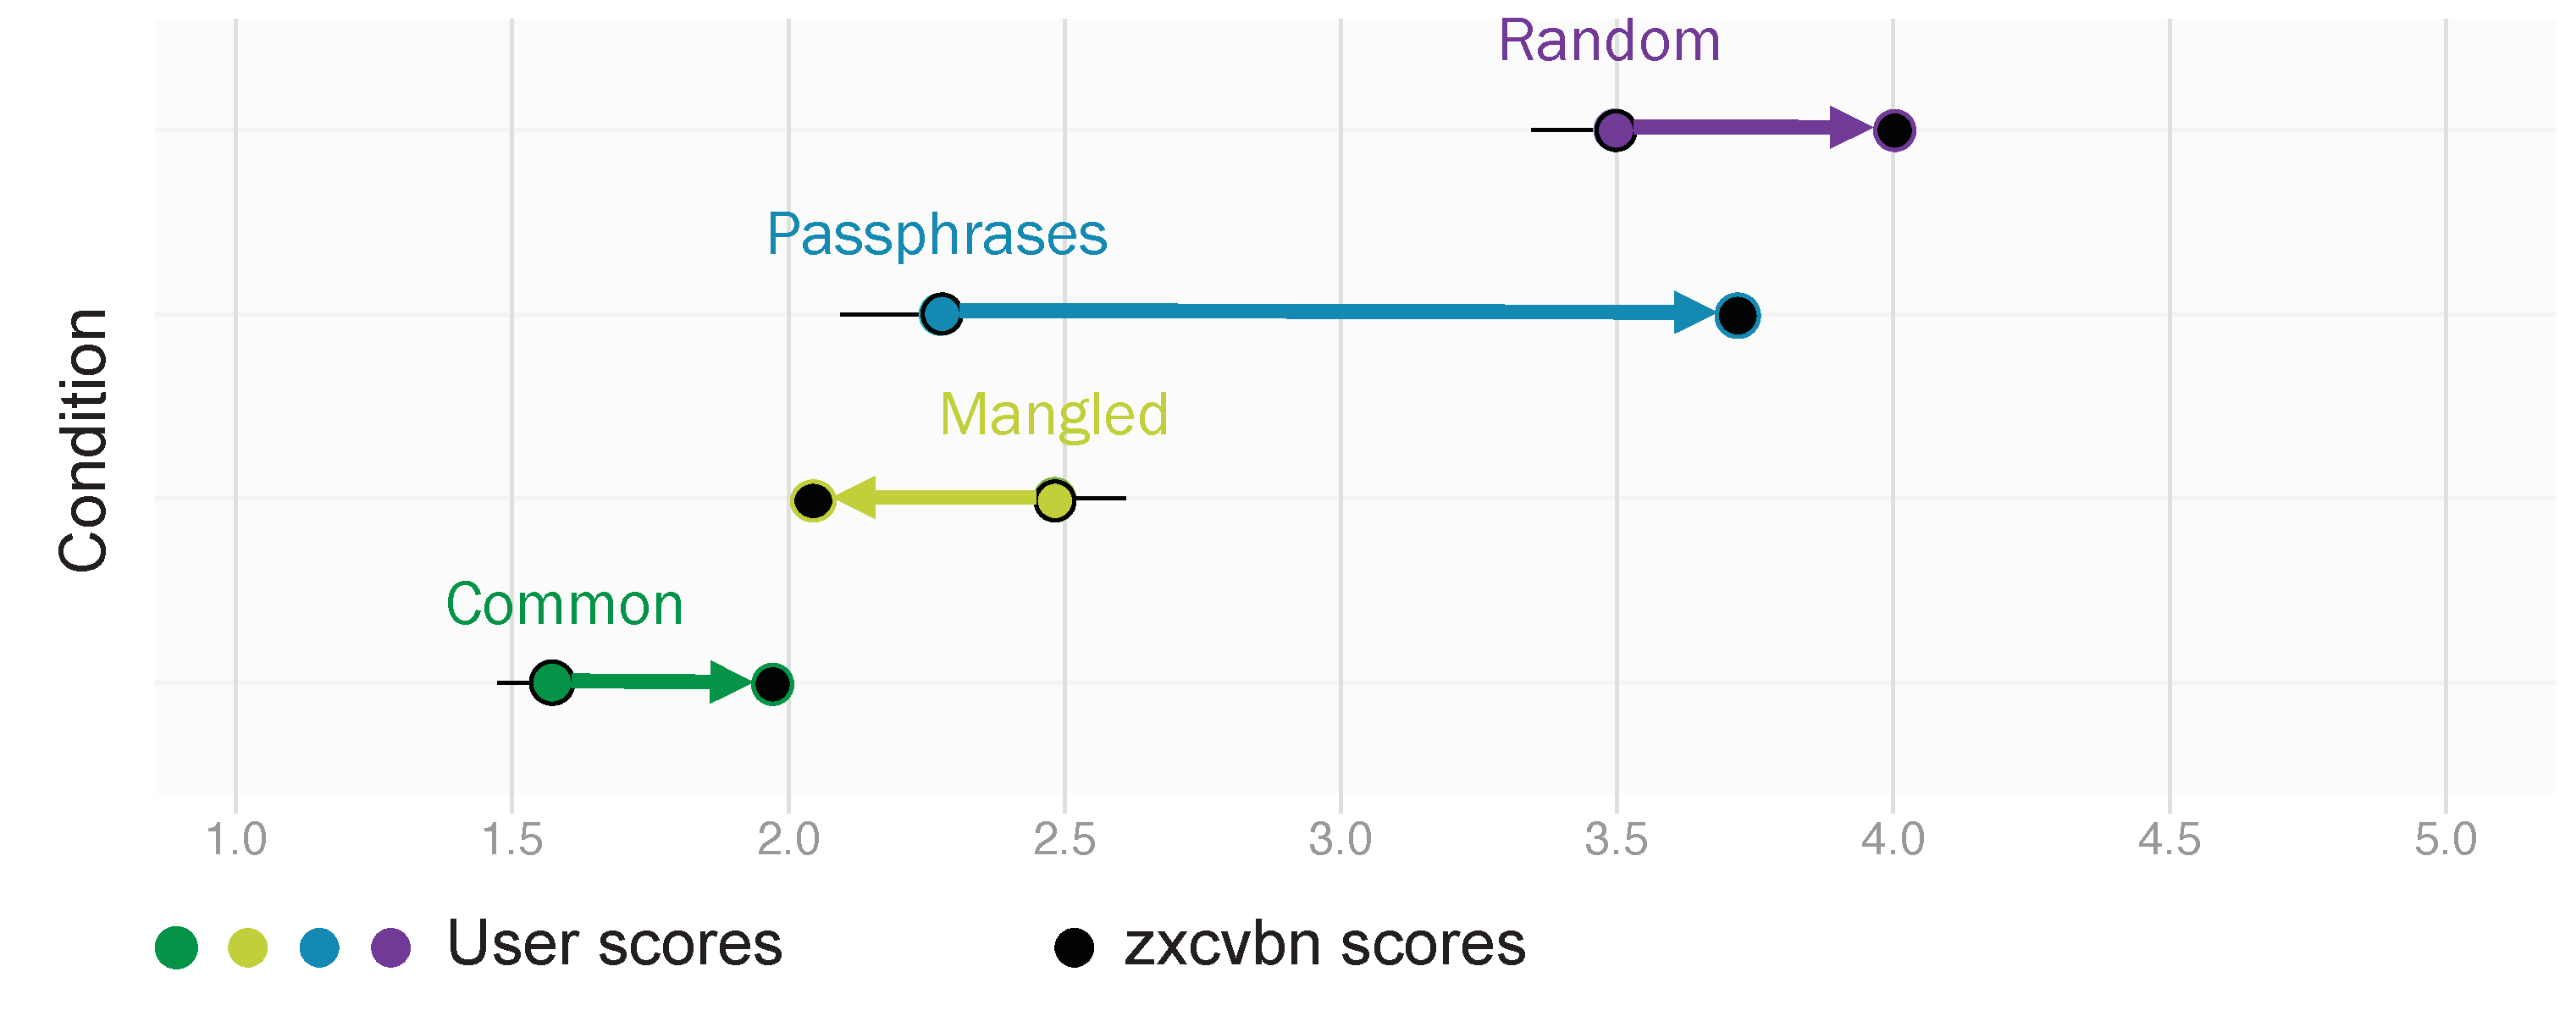
\includegraphics[width=\linewidth]{pasdjo/deviation-viz}
	\caption{\label{fig:pasdjo:deviation-viz} Average user ratings in each of the four conditions, plotted alongside mean zxcvbn scores. Users' estimations were least accurate for passphrases, which they had rated 1.4 points lower than zxcvbn. (N=111) }
\end{figure}

In their first game, players showed fairly consistent inaccuracies (see Figure \ref{fig:pasdjo:deviation-viz}) . Mangled passwords were the only condition that was overestimated (estimated median deviation $Md=0.5$). Interestingly, common passwords were underestimated slightly, although there was little room for underestimation ($Md=-0.5$). Random passwords were also underestimated by about half a point ($Md=-0.5$). The users in this data set rated passphrases exceptionally low ($Md = -1.6$). A Friedman rank-sum test showed significant significant differences for the deviations across the four conditions (\statslt{3}{187.84}{0.001}). We followed up this finding with Bonferroni-corrected post-hoc tests, i.e. $\alpha_{Bonf}=0.008$. Wilcoxon paired sample tests revealed significantly different deviations between all pairs of conditions, except for the common/random pair. In other words, common and random passwords were equally inaccurately assessed by the users. 

\subsubsection{Score Development}
From the 115 users who finished one game, 33 kept on playing for at least one more game. We tried to model their progress through a linear regression with gameIndex as predictor and achieved percentage as dependent variable. To account for the fact that some users played more rounds per game, we weighted the percentage with the number of passwords rated in that game. The model shows that players were able to improve their accuracy by playing multiple times (F(1)=49.37, \pvallt{0.001}, $\beta$ = 0.54, $R^2_{adj}$ = 0.23). Figure \ref{fig:pasdjo:percent-evolution} visualizes the progress of users who played at least twice. In there, it is also evident that the slope is not stringent, i.e. an individual user's accuracy does not necessarily increase steadily. We attribute this to the element of randomness in the game, which makes it more difficult in some cases to rate the passwords, while it might be easier in a subsequent game. 

\begin{figure}
	\centering
	\includegraphics[width=\linewidth]{pasdjo/percent-evolution-reg-multi}
	\caption{\label{fig:pasdjo:percent-evolution} Achieved percentage (accuracy) evolution depending on the number of games played. Each dot represents a full game of a user, the size of the dot indicates how many passwords were rated in that particular game. Although a linear model works, we used a locally weighted polynomial regression (LOESS) to fit a line through the data points. Users clearly become better the more they play.}
\end{figure}

%here we report on the findings as discussed in the OzCHI paper.

\subsection{Extended Sample and Results}
\begin{figure}
	\centering
	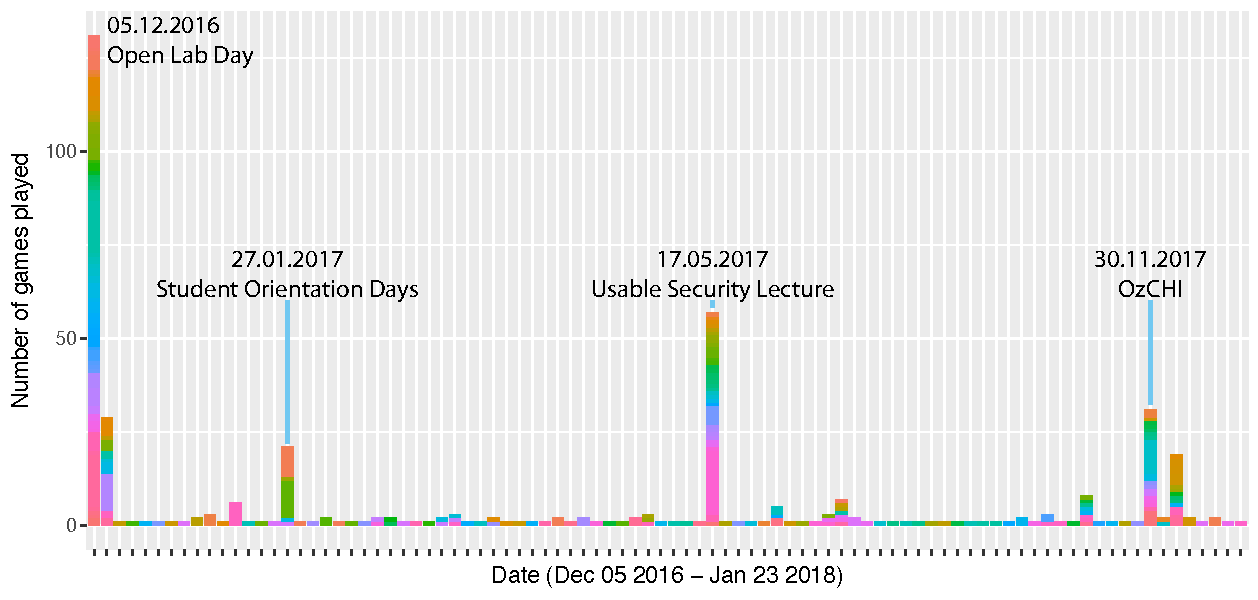
\includegraphics[width=\linewidth]{pasdjo/games-per-day-annotated}
	\caption{\label{fig:pasdjo:games-1y} The game was played on 90 distinct days (days with 0 games are not shown in the graph). There were four major drivers for the adoption (see annotations), that indicate that the sample mostly consists of students, their peers, and other academics.}
\end{figure}

On the 23rd of January, I created a new data dump and re-ran the analyses to see whether there were any differences to the first publication. The data set at this point consisted of 10,965 played rounds from 342 games played by 190 users on 90 distinct days (see Figure \ref{fig:pasdjo:games-1y}). Thus, there was an increase in 41.32\% in terms of games, and 85.38\% of played rounds. Before we look at the logs, we briefly present the changes introduced in PASDJO v2, which was deployed on November 7th 2017 (i.e. prior to the OzCHI conference, where the game was demoed)

\subsubsection{Version 2}
After publishing the first results, I had iterated the design and implementation of the game. There were a number of changes that might affect the players' performance. Splitting the data between v1 and v2 allows us to compare the players' performance before and after the adjustments to measure their effectiveness. 

\paragraph{New Condition: Predictable} The mangled passwords were algorithmically altered versions of common passwords. This often made it hard to figure out the original password. Perhaps, the mangled passwords sometimes seemed more like random passwords which is why they were the only overestimated condition in the first sample. The new condition ``Predictable'' mimicks the most predictable user alterations. The resulting passwords consist of a capitalized dictionary word with a predictable suffix, e.g. `123' or `!'. There were 12 predefined suffixes, and they were randomly appended to the dictionary word. 

\paragraph{Tuning Password Generation} After realizing that virtually no passwords had received a score of 5 in the first sample, I fine-tuned the generation of passphrases and random passwords. Passphrases were now either two or three words. Separators (e.g. a dash ``-'') were inserted in between the words. Random passwords used to be ten characters long in version 1. In version two their length is also randomized between 7 and 15 characters. This leads to a higher variety of zxcvbn scores. The resulting passwords sometimes resemble the mangled condition, which is a greater challenge for the players. Moreover, we increased the likelihood of common passwords from the top 100 by a factor of two. All measures resulted in a much more diverse spectrum of scores as shown in Figure \ref{fig:pasdjo:score-distribution-v2}.

\begin{figure}[htbp]
	\centering
	\includegraphics[width=0.7\linewidth]{figures/pasdjo/score-distribution-v2}
	\caption{\label{fig:pasdjo:score-distribution-v2}Zxcvbn scores in version 2. The scores within the conditions had become much more diverse, which should make it more difficult for players to judge individual passwords.}
\end{figure}

\paragraph{Scoring and Feedback} The players' achieved score ($A$) did not entirely reflect their performance. For instance, if a player rated as many passwords as possible without spending much thought on the strength, they still achieved a high score, albeit not a high accuracy. Therefore, the accuracy is now used as a ``penalty'' by multiplying the achieved score with the accuracy (e.g. $3000A~*~0.5P=~1500$ final score), which represents the performance much more adequately. Furthermore, the players had to figure out why their ratings deviated from the zxcvbn scores on their own. Now, the feedback screen contains a small indication as to how the score was calculated. This enables players to improve their score in the next game. 

\paragraph{Leaderboard and History} Finally, we introduced a new game-design element, namely leaderboards. Players can pick an alias and submit their score after each game. The main purpose of the leaderboard is to encourage \textit{competition}, which is another persuasive design strategy. 

%%%% SCORE DEVELOPMENT V2
\subsubsection{Score Development}
\begin{figure}[htbp]
	\begin{subfigure}[t]{0.49\linewidth}
		\includegraphics[width=\textwidth]{pasdjo/player-progress-multiplayers}
		\caption{\label{fig:pasdjo:1y-progress}Performance of players (Dec 2016 - Jan 2018)}
	\end{subfigure}
	\begin{subfigure}[t]{0.49\linewidth}
		\includegraphics[width=\textwidth]{pasdjo/v2-player-progress-multiplayers}
		\caption{\label{fig:pasdjo:v2-progess}Performance of version-2 players}
	\end{subfigure}
	\caption{\label{fig:pasdjo:v2-progess-comparison} Performance development during the first 13 months of public deployment (\ref{fig:pasdjo:1y-progress}). In November 2017, version 2 was released, where a linear model is a better fit (\ref{fig:pasdjo:v2-progress})}
\end{figure}
Among the players who played at least two games, the overall score development has not changed visibly (see Figure \ref{fig:pasdjo:1y-progress}), with no notable differences in the regression model 
(F(1)=67.12, \pvallt{0.001}, $\beta$ = 0.53, $R^2_{adj}$ = 0.23). However, if we look at the players who played version 2, we can observe a slight decrease in the model fit (F(1)=8.83, \pvallt{0.01}, $\beta$ = 0.43, $R^2_{adj}$ = 0.20): There were 12 players who played version 2 more than once ($M=2.9, SD=2.29$). Their progress is shown in Figure \ref{fig:pasdjo:v2-progess}. The decrease can be explained by the fact that only one player played more than three times in this reduced data set. %another user scored really really hight in their first game already, distorting the model 

%%%%%%%% Strength perceptions
\subsubsection{Strength Perception in the First Game}
\begin{figure}[htbp]
	\begin{subfigure}[t]{0.49\linewidth}
		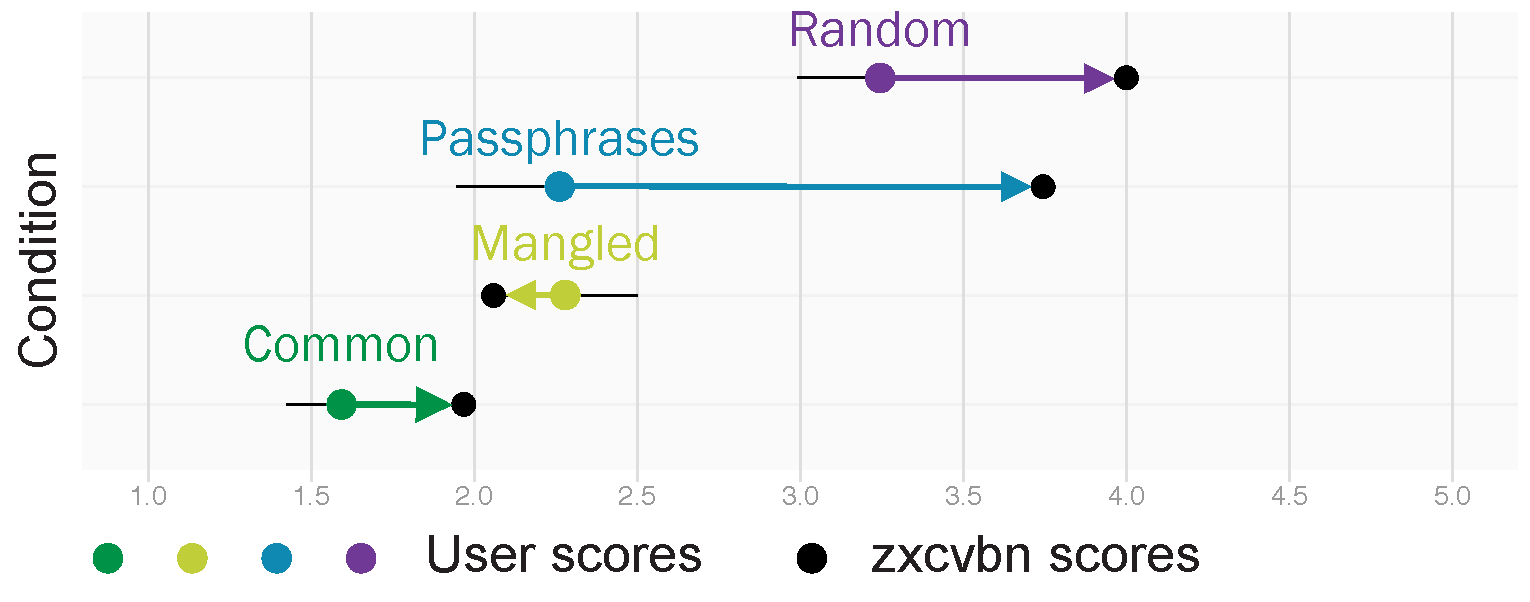
\includegraphics[width=\textwidth]{pasdjo/user-rating-v1-ci-annotated}
		\caption{\label{fig:pasdjo:1y-performance}Deviations of user ratings of v1 players.}
	\end{subfigure}
	\begin{subfigure}[t]{0.49\linewidth}
		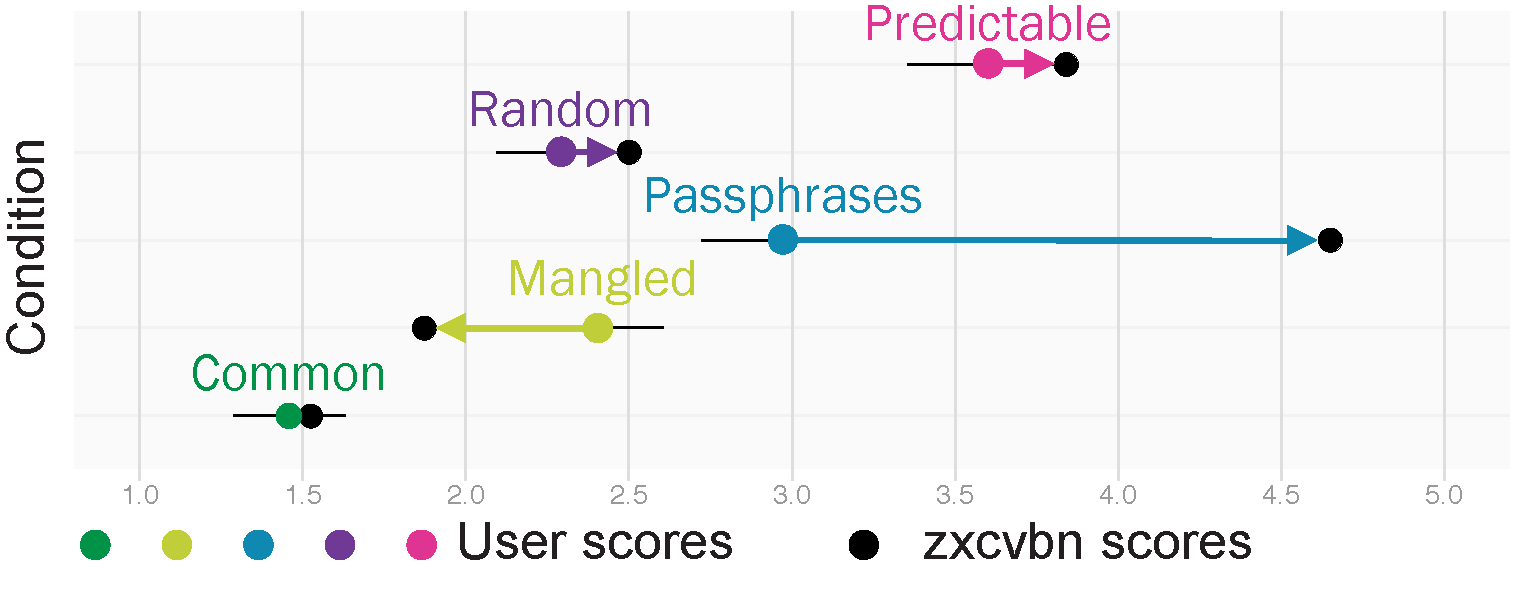
\includegraphics[width=\textwidth]{pasdjo/user-rating-v2-ci-annotated}
		\caption{\label{fig:pasdjo:v2-performance}Deviations of user ratings of v2 players.}
	\end{subfigure}
	%\caption{\label{fig:pasdjo:v1-v2-deviations}}
\end{figure}



\section{Discussion}

\subsection{Strength Perception vs. Selection}
- the data shows strong similarities to Ur \etal \cite{Ur2016PerceptionsPassword}
- perception and estimation of password strength appear to be easy for the players of our games even if they might not have a background in cyber security. 
- you rarely see passwords of other people, only when they share it with you. In many cases passwords that are shared with you are typically not the strongest passwords \cite{Haque2014Hierarchy,  Shay2010EncounteringPasswordRequirements, Singh2007PasswordSharing, Violettas2014PasswordsAvoidGreece, Weirich2001PrettyGoodPersuasion, ZhangKennedy2016RevisitingPasswordRules} 

\subsection{Intuition}
The time pressure and lead to users only spending 2.45 seconds on average per password. Can we assume that this indicates System 1 responded?

\subsection{Passphrases}
If you correctly identify a passphrase, you still need to count the number of characters to make a more informed decision about the strength estimation. The time pressure kept users from doing just that so we can safely assume that passphrases were rated very intuitively %TODO it would be possible to merge this section with the one above. 

\subsection{Changing users' mental models with PASDJO}
The learning effects clearly indicate that users learned assessing password strength after playing PASDJO. This makes us wonder if deploying such a game in different contexts, potentially in even shorter forms could effectively educate users. 

\section{Limitations}
\begin{itemize}
	\item were already addressed in new versions of the game. 
	\item used as an activity at Google	
\end{itemize}


\section{Summary}
\begin{itemize}
	\item users performed better than anticipated
	\item misconceptions mainly involve passphrases and mangled passwords
	\item the game was updated after the first results were in and is still deployed. Google even uses it internally. 
	\item the source code is available on GitHub.
	\item contribution: longitudinal data.
\end{itemize}


\subsection{Future Work}
Better onboarding
Challenges
Player Profiles 
adding the game to password management software

 %published
\chapter[Password Authentication in the Years 2016 and 2017]{Password Authentication in the Years 2016 and 2017}

\chapter[Survey: Policies against Reuse]{Survey: Policies against Reuse}\label{chap:policies-reuse}
\section{Background and Context}
\section{Method}

\section{Results}
\subsubsection{Policies are Mostly homogenous, with slight differences}
\subsubsection{Policies do not prevent password-reuse}

\section{Limitations}
 %published
\chapter[Password Personality]{Understanding Password Selection Through the Lens of Personality Traits}\label{chap:pws_and_personality}

%\section{Introduction}
% general introduction
% show that not *everyone* does the same
% selection is an individual task, not everyone selects passwords in the same way
Although there are certain patterns, password selection is a task that each individual handles in their own way. 
% even perception differs.
We have shown in chapter \ref{chap:pasdjo} that password strength is even subjectively \textit{evaluated} differently depending on certain characteristics. Again, while there was an overall tendency, we were not able to break down the strength ratings by individual differences: was there a special user group who performed better than others in the game? What characterizes this user group? Moreover, our previous chapter shed light on password policies in the wild. In a few notable cases, the rules were challenging and reject a substantial part of passwords. Users have developed strategies to cope with rejected passwords, but it would be interesting to know the exact factors that contribute to their behavior in these circumstances. Egelman and Peer make a strong argument that there is no ``average user'' so it is necessary to look at individual differences to understand user behavior \cite{Egelman2015AverageUser}. 

% personality traits in cybersecurity are a thing
Demographic background is one of the external factors that influences password selection \cite{Mazurek2013Measuring,  Violettas2014PasswordsAvoidGreece, Wang2015ChinesePWs}. Personality traits have been brought into the discussion to explain user preferences, actions, and behaviors in security questions \cite{Brown2004GeneratingPWs, Gross2016EffectCognitiveEffort, Shropshire2006PersonalityITSec, Zakaria2013DesigningEffectiveSecurityMessages}. Especially in research about phishing susceptibility we find evidence that personality traits have the potential to explain behavior \cite{Halevi2013PilotStudyPersonality,Halevi2015SpearPhishing,ParrishJr2009PersonalityPhishing,Uebelacker2014SocialEngineering}. 
% personality traits even matter for passwords
Empirical results from password studies have been discussed and explained with different personality traits, too \cite{Haque2014PsychometricsStrongPassword,Weirich2001PrettyGoodPersuasion}. It is a evident that a user's personality shines through, when they select a word based on personal preferences. 
% characterize personality in this realm
Petrie classified users in distinct password personalities: family-oriented, fans, fantasists, and cryptics\footnote{The original survey is not available online anymore. In a personal inquiry with Ms Petrie, she said that the original data is with the firm who commissioned the survey. The aggregated statistics are available at \url{http://passwordresearch.com/stats/statistic130.html}, \la{29.01.2018}}. A LastPass report more roughly divides password usage into two groups \cite{LastPass2016PersonalitiesGetUsHacked}: Type A users want to stay in control and are driven to act securely, so they developed an elaborate system that they perceive as suitable. Type B users do not believe that their accounts are valuable to attackers, so they do not prioritize security over usability. 
% this kind of categorization is nice, but too rough, maybe something more sound would solve the situation.
Those two taxonomies stem from analysis of user-selected passwords, i.e. a retrospective evaluation. However, predictive approaches are under-explored. For instance, if a user is generally an emotional person, does this impact their password selection strategies? If a user is diligent in real life, do they invest effort to diligently craft passwords, too? 
%``I can't remember passwords anyway'' could be attributed to a person who is less conscientious and/or less neurotic. 
%Are neurotic people more concerned about password strength, because they fear attacks more?

% that's what we do.
In a series of user studies we explored the associations between personality traits and passwords. If such associations exist, a new range of support systems opens that are tailored to a user's personality. Current one-fits-all approaches could be re-designed radically. The research was carried out in cooperation with three students. In each separate project we focused on a different stage of the password life-cycle. Timo Erdelt investigated personality as predictor for the usability of composition policies \cite{Erdelt2017BA}. Paul Huber explored correlations between strength perceptions and personality traits \cite{Huber2016BA}. Finally, Aline Neumann examined personality factors in password selection \cite{Neumann2017BA}. In total, 453 individuals participated in three separate online studies. In the following chapter, the projects are put into context and their findings are discussed on a bigger picture. 

\subsubsection*{Research Objectives}
Our primary goal was to find ways to predict password behavior from personality traits. At this point, the discourse about risky passwords included personality factors as explanatory variables. However, only few empirical studies had been carried out to challenge the assumptions. We aimed to provide such empirical data and a discussion of the implications on the design of password policies and password authentication systems. For instance, adjusting requirements of password policies depending on the user's personality promises to reduce frustration of password selection. Thus, our over-arching research question can be framed as ``\textit{Does personality influence user's mental models of password strength and selection strategies?}''.

%more related work: Groß \etal \cite{Gross2016CognitiveDepletion}
%
%Goals/motivation: 
%- some publications tried interpreted their findings as a consequence of different personality traits. first mentioned in \cite{Weirich2001PrettyGoodPersuasion} that personality could make a difference -- however, this had never been tried to empirically measure. 
%- explore differences in certain coping strategies (selection and reuse) through the lens of personality
%- find suitable ways to adjust password policies \cite{Seitz2017PersonalizingPasswordPolicies} - when users need to reset their password, after they had used the service for a while. 
%
%We posed the following research questions before we set out to conduct the study.\\
%\textbf{RQ1 - Psychological Factors} How much do psychological factors affect the perceived strength of passwords?\\
%\textbf{RQ2 - Big-Five vs GDMS} Are the Big-Five traits stronger or weaker predictors for strength perception than other psychological variables?\\
%\textbf{RQ3 - Portfolio Factors} Is the personal password portfolio associated with strength perception?

\section{Background and Related Work}
%We position our work in usable security and privacy, in particular password research. Moreover, we include psychological models to better understand users dealing with passwords. 
In this section we give a brief overview about the characteristics of strong passwords and how users go about creating them. Moreover, we portray projects in usable security and privacy research in which the users' psyche has been the focus. 
% secondary
%premise
%influencing 
%preconditions


%Moreover, since sophisticated attacks often start with checking for already known passwords, obtaining clear text data goes along with attackers improving their approach. A password that was strong before can quickly become very weak.  
%TODO eventuell noch das DING WANG paper und oder das Neural Network Ding vom Melicher zitieren.

%\subsection{Studies of Personality in Cyber Security}
\subsection{Password Selection Preconditions and Context Factors}
%TODO subconscious? 
%not exhaustive
% DEMOGRAPHICS
However, apart from such conscious behavior, there may be other preconditions that make some users pick stronger passwords than others. In a large field study, Mazurek et al. found that computer science and engineering students created passwords that were less guessable than those from business or politics students \cite{Mazurek2013Measuring}. Beyond demographic background, context factors like the emotional state during password selection have also been investigated. 
% EMOTIONS
Gulenko examined the effect of presenting positive textual messages and icons during password selection and found benefits for the adoption of passphrases \cite{Gulenko2014PasswordsEmotion}. In contrast, putting users in a state of cognitive distress or depletion made participants choose weaker passwords in a large lab study \cite{Gross2016EffectCognitiveEffort}. 
% PAST EXPERIENCES / BREACHES / ATTACKS
Social pressure as another type of psychological leverage was investigated by Egelman \etal \cite{Egelman2013DoesMyPasswordGoUpToEleven}. While they argue that account value plays a superior role for the effectiveness of password meters, others have shown that the \textit{design} of a password meter does have a measurable impact on the effort users put into creating a password \cite{Ur2012HowDoesYourPasswordMeasureUp}. In summary, the literature shows that password selection depends on context factors beyond education and experience. 
\subsection{Personality Factors in Cyber Security}
In our work, we are interested in context factors of password strength originating from psychological variables like personality. One of the most commonly used models to characterize personality are the Big-Five traits (B5), also known as the five-factor model. Costa and McCrae \cite{Costa1992NEO} refer to the personality traits as \textit{openness to experience}, \textit{conscientiousness}, \textit{extraversion}, \textit{agreeableness}, and \textit{neuroticism} (OCEAN). The traits can be described with these exemplary adjectives \cite{McCrae1987ValidationFFM}:\\
\textbf{Openness:} imaginative, creative, curious, independent, liberal\\
\textbf{Conscientiousness:} careful, reliable, ambitious, scrupulous, neat, punctual\\
\textbf{Extraversion:} sociable, talkative, passionate, warm\\
\textbf{Agreeableness:} selfless, helpful, forgiving, cheerful, humble\\
\textbf{Neuroticism:} worrying, emotional, insecure, impatient, vulnerable, subjective

Most frequently, the influence of these personality traits have been explored for privacy-concerns, where the openness trait was associated with privacy attitudes \cite{Egelman2015PredictingAttitudes,Minkus2014PersonalizationPrivacy}. Other inquiries have shown that personality traits like neuroticism \cite{Halevi2013PilotStudyPersonality} or openness \cite{Uebelacker2014SocialEngineering} might be associated with the response to phishing attacks. The likelihood of employees adhering to security policies is potentially influenced by the manifestation of agreeableness and conscientiousness \cite{Shropshire2006PersonalityITSec,Shropshire2015}. These investigations show that personality trait models are a considerable factor in security and privacy. Yet, our understanding of the influence of personality on password perception and consequently password selection is still low. Our work tries to improve our understanding about the origin of the differences in users' judgments of password strength. 
%is linked to these aspects, because passwords protect privacy of users and sensitive data of companies. %However, how password behaviors are formed and how much of the  is explained by psychological factors is still underexplored

%%%%%%%%%%%%%%%%%%%%%%%%%%%%%%%%%%%%%%%%%%%
%%%%
%%%%
%%%%			STUDY  1 ONE EINS
%%%%			POLICIES
%%%%
%%%%
%%%%%%%%%%%%%%%%%%%%%%%%%%%%%%%%%%%%%%%%%%%
\section{Study 1: Policies}
% general motivation - why do we investigate this?
We start out with the exploration of psychological factors for the design of password policies. We were motivated by the fact that at this point, policies are a one-fits-all solution that evidently does not work in the same ways for all users: Shay \etal observed that subjective usability ratings for policies differed among participants \cite{Shay2012CorrectHorseBatteryStaple, Shay2014CanLongPasswordsBeSecureAndUsable}. For instance, about 40\% of their participants found it difficult to create a password under a ``3class16'' policy, but another 40\% found it easy \cite{Shay2014CanLongPasswordsBeSecureAndUsable}. Following the general discourse and related results from privacy research, we hypothesized that an individual's personality might be responsible for their attitudes towards one policy or another. Therefore, our goal in this project was to explore such associations between personality traits and policy preference. 
%GOALS: explore associations between big-five traits and password selection under different policies, both on usability and security metrics. Investigate the effects of using a non-traditional password policy based on emojis. user preference for one policy or another. explorative study so no p-values.
\subsection{Method}
% general methodology
Our study was completely exploratory, because the literature did not allow us to derive narrow hypotheses. Since personality traits are nuanced, we opted for an online survey to collect a larger sample. Personality was assessed in the Five-Factor Model. We opted for the BFI-K construct by Rammstedt and John \cite{Rammstedt2005BFI}, because it is freely available in German. Moreover, with its 21 items, the time to fill out the questionnaire is kept reasonably low. 
Participants were asked to create several passwords in a row, i.e. the study followed a within-groups protocol. Here, we evaluated three different password policies: a traditional (3class12), an uncommon (2word12), and a novel policy (emoji12) that required the selection of at least one emoji through a graphical user interface (more on emojis in chapter \ref{chap:emojipasswords}). The reason for this choice was that the policies are different enough to serve as levels of the independent variable ``policy''. Participants assessed the ``difficulty to create'' a password for each policy. Moreover, we had them rank the policies by their personal preference, so the choice of 3class12, 2word12, and emoji12 would help them spot and judge the differences easily. 

\subsubsection{Structure and Tasks}
The study was divided into 3 overall parts. In the first part, participants were briefed about privacy details of the study and they provided demographic background information. Then they proceeded to the personality questionnaire before they were asked to perform three experimental tasks. Each consisted of creating a password and assessing the difficulty with agreement levels on the three items \textit{``It was difficult to create a password that meets the requirements''}, \textit{``I found the password requirements bothersome''}, and \textit{``It was easy to create a \textit{new} password''}. Agreement was measured on a five-point scale ranging from ``Strongly disagree'' to ``Strongly agree''. Inversely keying the items as well double encoding makes the data more robust against implausible responses. 

The order of the policies was counterbalanced to mitigate order effects, we recorded the order as a control variable. We chose an online-banking scenario for all three selections. The first prompt was to create a password to protect an online banking account. Secondly, participants were told that someone had gained access to their account and the bank locked them out. As a security precaution, they had to reset their first password. The last task description explained that their password had expired after one year and they need to reset it again. This storyline was designed to fulfill the \textit{realistic threat} principle proposed by Krol \etal (see Section \ref{sec:rw:principles-experiments}) \cite{Krol2016ExperimentDesign}. 

We used SosciSurvey, a standard survey tool, to collect the responses. The dynamic parts involving password selection were embedded in iframes. To match the data from the survey tool and the iframe we used URL query parameters containing the response ID. We asked participants to switch to a desktop browser to avoid styling glitches and unexpected behavior from the prototypes. %Auto-complete was prevented in any case

\subsubsection{Recruiting and Demographic Background}
We recruited participants through posts on social networks and by sending out the invitation link in a university-wide newsletter (more than 5000 recipients). To incentivize participation, we announced a raffle of five shopping vouchers with a value of 20€ each. At this point, 222 people had started participation. After drop-out and plausibility checks, the remaining sample size was $N=164$. As expected, the age distribution was narrow: our sample consisted mostly of students in their mid-twenties \average 24.7 (SD=5.5). 79 respondents were female, 83 male, and 2 preferred not to answer. In the background screener, 65 people (40\%) indicated to possess formal training in computer science or information technology. We also requested self-reported assessments on password behaviors. Here we found that 40\% reuse passwords without modification, 32\% reuse them with modifications or with a mnemnoic technique. 17\% often create new passwords. In terms of management strategy, the majority (53\%) tries to memorize passwords. 11\% use a password manager or generator. Written cues served as aid for 10\% of respondents, and 16\% write passwords down on analog media, while 21\% use electronic files. Interestingly, the distribution of coping strategies is very close to survey findings gathered with more diverse samples \cite{CSID2012PasswordHabits}. Hence, we believe to have caught a representative snapshot of password behavior.

\subsubsection{Statistical Analyses}
For statistical analyses, we consulted the StabLab\footurl{http://www.stablab.stat.uni-muenchen.de/}{30.01.2018} to identify suitable methods. After a revision of the collected data and the necessary assumption checks, the associations were explored with additive models (AM). Their advantage over linear regression is more flexible for non-linear associations \footurl{https://en.wikipedia.org/wiki/Additive_model}{30.01.2018}. The \textit{mgcv} package for R was used to calculate the models.

Scores on the Big-Five sub-dimensions served as independent variables, i.e. the predictors in the regression models. \textit{Openness} is coded with five items, while the remaining four dimensions were assessed with four items. The agreement levels for each item were mapped to numeric values from 1 to 5. The score on a sub-dimension is the sum of agreement levels. To better estimate effect sizes, we control for gender, age and IT proficiency in the models. 
\subsubsection{Method limitations}
The method, albeit carefully executed, faces a few limitations regarding the interpretability. First, the sample was fairly homogeneous, because participants were mostly between 20 and 28 years old and have an academic background. However, personality traits are not age dependent \ar?. Our study was strongly focused on individual preferences and usability perceptions of different policies, so only a within-groups design was feasible. However, in real-life password selection, users rarely select three passwords in a row. The choice of our storyline still makes confident about the ecological validity \cite{Fahl2013EcologicalValidityPasswordStudy}. The repeated measures design did not allow us to measure the policies' influence on password memorability, which we have to postpone to another study. At this stage, the preference was more valuable for our exploration than memorability effects. Besides, we briefed participants to fill out the survey on a desktop PC or a similar device. We cannot guarantee that all participants followed this instruction, which might have had an effect on their password selection \cite{Melicher2016UsabilityMobileTextPasswords}. 

Finally, we unfortunately made a mistake in the deployment of the emoji-based policy. Instead of 12 characters, it required participants to select 16 characters beside the emoji. We realized this fact by looking at descriptive statistics during the course of the study, because the policy performed significantly worse than the other two. We re-deployed the emoji-based policy immediately after we had realized the error. Consequently, we had to remove the data for the creation difficulty and ranking in cases 1-61, reducing the overall sample size to 103. Nonetheless, the sample size is sufficiently large to investigate medium to strong effects. 

%- we started out with emoji16, but made the switch to emoji12 (after 43 participants), because emoji16 received the most negative feedback, but it was mostly due to the length. data removed for ranking (1-61) and difficulty to create (1-43). 

\subsection{Results}


medium associations between extraversion, agreeableness, and neuroticism (basically the other three dimensions that were not useful before), but control variables are associated to a larger degree.

emoji policy similar results as traditional policies, i.e. it is wortwhile to experiment with it

\paragraph{Descriptives and Hypothesis Tests}
creation difficulty: Repeated measures linear mix model ANOVA. random intercept to account for the fact that people generally rate policy usability low. baseline (any could be chosen) emoji 12.

emoji \average 7.89 (in [3;15] range), 2word12 + 0.12, 3class12 - 0.70 (easier)
serial positioning effects do make a difference, but it also appears trivial in the overall sample.
summary: no big difference between policies and ranking. (this is what makes the remainder more exciting, because a closer look at the data brings out how the numbers come to be)


\paragraph{Creation Difficulty}
% gender
Female participants reported more difficulties for emoji12 ($\beta=0.91$) and 2word12 ($\beta=1.35$). 
for 3class12 correlation was smaller ($\beta=-0.46$) and pointed in the opposite direction.
% it background
IT background revealed interesting effects too: emoji12 ($\beta=-0.10$) trivial, 3class12 ($\beta=0.21$) weak, 2word12 ($\beta=0.61$) medium. it looks as though people with higher IT knowledge struggle with a word-based policy, potentially because it is much less common in the wild. 
% order of the policy
If you factor in the order of the policy, the results look clearer. if emoji12 and 3class12 were shown in position 2, creation was more reported to be more difficult emoij12-2 ($\beta=0.52$), 3class12-2 ($\beta=1.19$) 
% age
we observed non-linear associations between age and creation difficulty, but the small age range forbids us to make conclusive inferences from our data.

%emoji personality
mostly non-linear associations for the emoij12 policy
neuroticism weak linear association emoji12 ($\beta=-0.22$), i.e. it was slightly easier for people with higher neuroticism scores (this is a great result, albeit weak. neurotic people are by defintion more \textit{emotional}, and emojis seem to cater to this trait.)
agreeableness weak non linear, and interesting curve (up and down) for emoji12
openness weak non linear, but too little data to conclusively decide. 
% 2word12 personality
effects not as clear as for the emoji policy. highly open people report slightly less difficulty to create a 2word12 password.

% 3class12
linear associations are negligible for extraversion, conscientiousness, and neuroticism. 
non-linear associations for agreeableness and openness. at value around 15 (from 20) the difficulty seems to increase (hard to interpret this finding). People with agreeableness scores of 18 and greater find it more difficult to create a 3class12 password by up to 1.5 points. Openness is inversely correlated here. the more open the participant was, the more likely they found it easy to create a 3class12 password. 


\paragraph{Ranking}
logistic additive regression %https://web.stanford.edu/~hastie/Papers/AdditiveLogisticRegression/alr.pdf
did policy X land on top spot ? yes = 1, no = 1. thus, no encompasses the two other options.
Logit model. see timo's work to better understand what's going on. 

\begin{table}
	\centering
	\caption{\label{tab:pws_pers:distribution-binary-ranks} Distribution of binary rankings of the three available policies. Evidently, 3class12 was ranked best in most cases. }
	\begin{tabular}{llll}
		~ 			& emoji12	& 2word12 	& 3class12 \\ \hline\hline
		1st rank	& 18		& 12		& 67 \\
		other rank 	& 80 		& 85 		& 31 \\ \hline
		n			& 98		& 98		& 98		 
	\end{tabular}
\end{table}


% predictors: demography and structure
strong effects. the probability of a non-IT person putting emoji12 at the top is $exp(\beta–{IT-0}=9.87)$, so around ten times higher. only one IT-person ranked emoji12 first. (this fits to the finding that non-IT people found it easier to create an emoji12 password).
% order of policies 
the order in which policies were displayed also produced a notable effect. If emoji12 is shown in 2nd $exp(\beta–{emoji-pos2}=0.27)$ or 3rd position $exp(\beta–{emoij-pos3}=0.76)$, the likelihood to rate it the best policy slightly decreases. Other positionings, as well as age-related preferences, were inconclusive.

% personality
generally weak associations.
extraversion, weak linear effect regarding 2word12. likelihood to put 2word12 first decreases with higher extraversion scores $exp(\beta–{E-1}=0.82)$. for agreeableness both linear and non-linear effects are visible; higher scores increase chances to vote emoji12 first $exp(\beta–{A-1}=1.28)$. openness or conscientiousness have negligible, random associations. for neuroticism we lack data in edge cases (low or high trait scores) to draw conclusions. %there are more results in the BA, but I do not really see the point of reporting all the details of inconclusive results


\paragraph{Password selection}

\todo{create a emoiji selection histogram}. In essence, some emoji were strongly preferred, e.g. the red heart and the ``pouting face''. analyze: what were the usability ratings/rankings of those who picked the heart vs. the pouting face, i.e. are emojis with a positive connotation used by people who are happy that they can select an emoji password? I guess there are significant effects here. 

\subsection{Lessons Learned}
It could have been useful to include a recall test à la ``which passwords do you still remember after filling out the personality questionnaire?'' 

\subsection{Discussion}
%TODO re-read the discussion section, because the findings are a bit higher level and more understandable
Most interesting finding: Non-IT people significantly less likely to put emoji policy first. s

emoji (negatively) associated with emotional stability, i.e. less stable people who are more emotional in either direction were more positive towards emojis.

non linear associations probably explicable by other variables, e.g. intercorrelation -- 
\todo{discuss the personality traits and associations, try to explain them.}

demographics play a role - (careful now, cowboy): policies could be tailored to gender. but i'm kind of reluctant to put this argument forward. at least IT background could be considered a factor for the policy. a personalized policy would make it more difficult for horizontal attacks because the policy is unpredictable.

mutually exclusive effects for ranking are clear because of the binary nature.

wild idea: if positioning influences the favorability of policies, one could leverage this. like anchoring and decoy (chose your own policy of the three). commitment and consistency as well (commit to your policy, create a strong password to be consistent with your commitment.)

%%%%%%%%%%%%%%%%%%%%%%%%%%%%%%%%%%%%%%%%%%%
%%%%
%%%%
%%%%			STUDY  2 TWO ZWEI
%%%%			PERCEPTION
%%%%
%%%%
%%%%%%%%%%%%%%%%%%%%%%%%%%%%%%%%%%%%%%%%%%%
\section{Study 2: Strength Perceptions}
With an observational online study, we explored the associations between psychological variables and password strength perception. As outlined in Chapter \ref{chap:pasdjo}, we regard the perception of strength as an implicit driver for behavior, which is more difficult to observe. Hence, we explored associations between subjective password strength ratings and scores on well-established psychometric scales. 
%task description
The task resembled the PASDJO game: participants were shown a password, and they had to rate it on a seven-point scale. We chose seven point scales to make the approach more comparable to Ur \etal \cite{Ur2016PerceptionsPassword}. Moreover, we gave participants two passwords, and they had to decide which one was stronger. 

%pre-registration
Before we ran the study, we pre-registered the experiment with the open-science framework (OSF)\footnote{\url{https://osf.io/}, last accessed 11.09.2016} and planned to conduct all analyses as predicted to mitigate confirmation bias. However, the envisioned statistical  tests were not always applicable, which forced us to consider more appropriate methods and move away from the pre-registration. Since we consider our research efforts mostly exploratory, we approached the study without specific hypotheses regarding the influence of certain personality traits on the perception of password strength.

\subsection{Structure}
% First Part: DEMOGRAPHICS
The study was divided into six parts. Two parts were standard psychometric tests. We describe all parts, to give the reader the full picture about the participants' tasks. However, we have to omit a few less important results for the sake of clarity. After a brief introduction where the participants were informed about the background of the study, the first step was to provide basic demographic information regarding gender, age, educational and professional background. %This information is important for the ratings on the password scales, because advanced knowledge in IT(-security) may lead to a different rating than the general audience. 

% Second Part: META STATISTICS / CREATION
\paragraph{Meta Password} The second part elicited characteristics about the passwords that our participants used on real online accounts. Here, we asked about typical password attributes, like LUDS (lower-, uppercase, digits, symbols), length and the inclusion of dictionary words. The collection of such password descriptions is an ethically reasonable way to study actual behavior that does not directly involve creating and disclosing an entire password \cite{VonZezschwitz2013SurvivalShortest}. Participants could select from a list of accounts that they used on a regular basis, e.g. Facebook, YouTube, Netflix, Google. If they did not have any of the selectable accounts they could provide another. We call the description of a participant's password on any of these sites ``\textit{meta password}'' in the remainder of the chapter. We included this part in the survey to explore additional covariates for strength perception.
%TODO entscheiden ob das reinkommt Additionally we had them create a password which they would rate as sufficient to protect such an online account and that is memorable. We asked not to enter a password that they were currently using. At the end of the study, we again inquired after the fictional password to measure short-term memorability. 

%%% TABLE: PASSWORDS
\begin{table}[htbp]
  \centering
  \caption{Set of passwords that we divided into different length and strength categories (as measured with zxcvbn). Features: U = uppercase, D = digits, S = symbols}
 % \small
    \begin{tabular}{lllcccr}
    \multicolumn{1}{c}{\multirow{2}[1]{*}{Password}} & \multicolumn{2}{c}{Categories} & \multicolumn{3}{c}{\multirow{2}[1]{*}{Features}} & \multicolumn{1}{c}{guesses} \\
      & Length & Strength & \multicolumn{3}{c}{} & \multicolumn{1}{c}{(log10)} \\
    \midrule
    hagrqqqqthhbbe & Long & Strong & \multicolumn{3}{c}{-} & 12.48 \\
    etuhcarap & Short & Weak & \multicolumn{3}{c}{-} & 4 \\
    AbWxCdYz & Short & Medium & \multicolumn{3}{c}{U} & 8 \\
    1qaz2wsx3edc & Long & Weak & \multicolumn{3}{c}{D} & 3 \\
    a6a4ba8a & Short & Medium & \multicolumn{3}{c}{D} & 8 \\
    ieatkale88 & Short & Medium & \multicolumn{3}{c}{D} & 10 \\
    thedzfhg123 & Short & Medium & \multicolumn{3}{c}{D} & 10 \\
    11Nd1sPPut8ble99 & Long & Strong & \multicolumn{3}{c}{U,D} & 16 \\
    bicycles-peaches-cold & Long & Strong & \multicolumn{3}{c}{S} & 13.69 \\
    AatIcs,ijayl-t & Long & Strong & \multicolumn{3}{c}{U,S} & 13.95 \\
    p@ssw0rd & Short & Weak & \multicolumn{3}{c}{D,S} & 0.95 \\
    ocean4 Size !beer Car & Long & Strong & \multicolumn{3}{c}{U,D,S} & 20.39 \\
    F@m1Ly07\% & Short & Medium & \multicolumn{3}{c}{U,D,S} & 6.88 \\
    \bottomrule
    \end{tabular}%

  \label{tab:password-list}%
  
\end{table}%

% Third Part:  RATING
\paragraph{Standalone Strength Rating} In the third part of the study, the \textit{rating part}, the participants assessed the strength of one password at a time in random order, similar to playing PASDJO. The passwords had to be rated on 7-point scales ranging from \textit{1 = very weak} to \textit{7 = very strong}. We picked a set that was comparable to related work \cite{Ur2016PerceptionsPassword} and that we carefully designed around certain attributes. Table \ref{tab:password-list} shows the selected set of passwords and their features. The ``length'' category distinguishes between short passwords with nine characters or less and long passwords with ten characters or more. The distinction is inspired by real-world policies that most commonly require up to nine characters (see Chapter \ref{chap:policies_reuse}). The ``strength'' category groups passwords on three levels by their guess number as determined by zxcvbn. Weak passwords require less than $10^{6}$ guessing attempts, strong passwords at least $10^{12}$ guesses, and medium passwords anything in between. This classification is in concordance with related work \cite{Florencio2014AdministratorsGuide, Wheeler2016zxcvbn} . To fully counterbalance all category combinations, one would require 120 items, which we could not implement for the sake of brevity. Hence, we kept the number of items small to mitigate fatigue during the study sessions. In the chosen set of 13 passwords, there were at least three items for each distinct category, i.e. three short, long, weak and strong passwords, and at least three passwords pertaining to different LUDS policies (lowercase, uppercase, digits and symbols).

% Fourth Part: COMPARISON
\paragraph{Comparison} Following a similar procedure as Ur et al. \cite{Ur2016PerceptionsPassword}, participants moved on to compare the strength of passwords pairs (\textit{comparsion part}). The 7-point scale ranged from ``<left password> is much stronger'' to ``<right password> is much stronger''. The pairs were constructed such that the passwords differed, e.g., in the existence and positions of digits and uppercase letters. Figure \ref{fig:comparisontask} illustrates our scoring schema. 

\begin{figure}
	\centering
	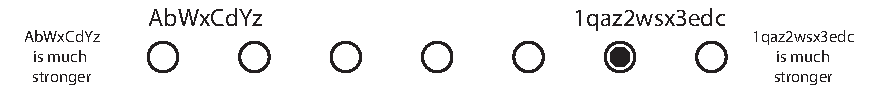
\includegraphics[width=\linewidth]{figures/comparisontask}
	\caption{\label{fig:comparisontask} Simplified item of the comparison task. The passwords differ in length, strength, and the usage of uppercase letters and digits. Here would have scored the importance of length and digits with +2 while the importance of strength and uppercase letters was scored with -2.}
\end{figure}

If the passwords measurably differ in strength as in Figure \ref{fig:comparisontask}, the ratings show if the participants' perceptions match reality. In total, ten comparisons had to be made in random order, in which we permuted the combinations. For this task, we also added an attention check where the passwords on both sides of the scale matched, allowing us to exclude responses where the answer differed from ``both passwords are equally strong''. 

\paragraph{SeBIS} Next, we requested self-assessment about security-related behavior using the Security Behavior Intentions Scale (SeBIS) \cite{Egelman2015SeBIS}. This scale comprises the dimensions \textit{securement}, \textit{passwords}, \textit{awareness}, and \textit{updating}. For each dimension, a score is calculated with four items totaling up to 16 additional items in our study. However, in discussions after the experiment we received hints that it would have been better to include a gap of a couple of days before collecting the SeBIS data to ensure its validity. Since we failed to take this into account beforehand, we do not report the results further, but it is important to mention that the questionnaire included those 16 items. 
%The items are phrased as statements to which respondents can indicate how often they show a certain type of security-related behavior. The scale ranges from \textit{1 = never} to \textit{5 = always}. The \textit{password} dimension measures general attitude towards passwords, which we can utilize to inform our interpretation later.

\paragraph{Big Five} The study concluded with two psychometric tests. In the \textit{Big-Five part}, we utilized a set of 50-items from the International Personality Item Pool (IPIP), which is a representation of Costa and McCrae's NEO-PI-R domains \citep{Costa1992NEO}\footnote{All items of the personality test can be found here: \url{http://ipip.ori.org/newNEODomainsKey.htm}, psychometric properties: \url{http://ipip.ori.org/newNEO_DomainsTable.htm}}. In this personality test, participants rate how accurately a certain statement portraying a certain personality characteristic describes themselves. Each item is a 5-point scale with the labels \textit{very inaccurate, moderately inaccurate, neither accurate nor inaccurate, moderately accurate, very accurate}. Every personality trait is tested with five positively and five negatively keyed items. It was shown that the 50-item version of the test shows high correlation with more exhaustive tests ($r > 0.75$ in all dimensions) and is thus a sufficiently reliable test. We randomized the order of the items.

\paragraph{GDMS} Egelman and Peer found that the general decision-making style had higher predictive power than the Big-Five traits for privacy-related behavior \cite{Egelman2015AverageUser}. Thus, we wanted to test the feasibility of both psychometric tests and finished the study with the \textit{GDMS part}. This scale uses 25 positively keyed items to measure the five decision-making styles \textit{rational}, \textit{intuitive}, \textit{dependent}, \textit{avoidant} and \textit{spontaneous}. 



\subsection{Quantitative Analysis}
Since at least three passwords showed a certain characteristic, e.g. uppercase letters, we averaged the ratings for them accordingly and used them as dependent variables. Moreover, in the psychometric tests we accounted for negatively keyed items, i.e. those items that were phrased with negations like \textit{``I don't talk a lot''}. We inverted the ratings where necessary and afterwards calculated the sum of agreement levels for each dimension (\textit{trait score}). 

%cleaning the data
As in Section \ref{sec:personality:study-1}, we repeatedly fit a \gls{GAM} to our data, i.e. a more flexible and interpretable form of regression\footurl{https://multithreaded.stitchfix.com/assets/files/gam.pdf}{06.02.2018}. 
%DV
Subjective password strength assessments, respectively comparisons, serve as dependent/response variables. We calculate one score per participant and password category by adding up the corresponding ratings. For instance, if they rated all eight passwords containing digits with seven points, their score for ``G\_Digits'' (\textbf{G}roup of passwords with digits) is 56. We average participants' ratings for models that require means instead of total scores. 
%Only to compare the means in each password category, we average the ratings. 

%IV
Psychometric scores on all several sub-dimensions served as independent variables (covariates). We always control the regression models for gender, technical background and age to contrast effects. Wherever possible, we model covariates as linear, if the GAM indicates that smoothing is unnecessary. For this data-set, we also conducted principal component analysis followed by factor analysis. The resulting factors are then used to fit additional models for comparison. This allows us to evaluate the suitability of the Big Five inventory for our exploration.
%Since some \gls{GAM} smooth terms might make models worse, we use automatic penalization to basically remove them from the model\footurl{https://www.rdocumentation.org/packages/mgcv/versions/1.8-23/topics/gam.selection}{06.02.2018}. 

%We check for collinearity using variance inflation factors (VIF) and only retain factors with VIFs close to 1 \cite[p. 217]{Weisberg2005applied}. 
%Finally, we perform Durbin-Watson tests to rule out auto-correlation effects (target value $d=2$). While p-values do not add much to the interpretability of the findings, we report them for the sake of completeness.  
%TODO Quelle!
%Our level for statistical significance is $\alpha = 0.05$, unless Bonferroni correction requires a lower value. 

%When we report the results of linear regression models, we only do so for the models with the highest adjusted $R^2$ value, i.e. the model where the number of predictors leads to the best model-fit explaining the variance in the dependent variable. The values in Tables \ref{tbl:personalpw_regression} through \ref{tab:Comparison-Regression} are the \textbf{standardized beta} correlations, i.e. they are unit-less and lie between -1 and +1. 

\subsection{Qualitative Analysis}
To better understand the reasoning behind the ratings and comparisons, we also inquired how the respondents approached the rating task. They could enter free-text answers after all ratings were done. The answers were then coded independently by two members of the team. The first coding step was to find categories and propose the code book. Afterwards, the proposed codes were handed over to the second coder, who sorted answers into the categories and amended new ones where necessary. Interrater agreement between the two coders was satisfactory (78\%, Krippendorff's $\alpha = 0.55$) and the final the code book could be created after discussing the discrepancies. We report how many participants mentioned a particular theme in their response regarding their rating strategies.


\subsection{Recruitment}
We utilized the online research platform Prolific\footnote{\url{https://prolific.ac}, accessed 01.09.2016} to administer our survey. Participants received \$2.65 upon successful completion, which took 20 minutes in average. This compensation level is suggested as part of the ethical reward guidelines on the platform. Only an English-speaking audience was eligible to participate. From the 178 people who started the survey, 104 finished it. To prevent low quality answers, we introduced an attention check during the comparison part of the experiment.  



\subsection{Ethical Considerations}
There is no institutional review board for this kind of studies at our institution. However, we designed the questionnaire to respect the participants' privacy and did our best to minimize the level of disclosure of sensitive data. The metrics we collected to characterize the participants' passwords are most likely insufficient to reconstruct the passwords in a straightforward way and can thus be considered ethically acceptable. 


\subsection{Limitations}
%It is good to discuss the limitations before the results. Thus, the reader can bear them in mind when they are reading on. 

Like most studies involving personality assessment, the result is only a rough model of a person's personality and does not include all facets. We chose a test with 50 items to assess the Big-Five traits. While such psychometric tests exist with item counts between 10 \cite{Gosling2003TIPI} and 240 items \cite{Costa1992NEO}, the 50-item version has high internal reliability and does not fatigue the respondents as much as more exhaustive tests. Additionally, with a sample size of 100 participants, power-analysis tells us, that only strong and medium interactions are likely to be found for with our regression models (cf. \cite{Shevlin1998SampleSize} or \cite[p. 223]{Field2005DiscoveringStatistics}). At this stage of the exploration, however, this is what we aimed for. If we do find effects with such a small sample, then they must be large enough to justify follow-up investigations with larger samples. Moreover, statistical analyses can be done very differently. We traded off model complexity and interpretability to draw first conclusions. Thus, the reported associations can never be seen \textbf{causal effects}, because we would have to use different experimental setups, and carry out the experiments many times on larger samples. In the scope of our personality studies, we therefore provide pointers and possible explanations, but do not claim that the results are highly generalizable. This is especially important, because the sample stems from a technically savvy audience. Users registering for tools like Prolific or Amazon Mechanical Turk may also have stronger financial motivation to do so than the rest of the population \cite{Ross2010WhoAreTurkers}. 

Furthermore, the methodology relies on self-assessment and honest answers, which are difficult to control. We introduced an attention check to mitigate the problem, by asking people to compare two identical passwords. For the meta-password, we do not know whether it was created on a mobile or desktop device. Passwords created on mobiles are usually less complex than those created on desktops \cite{Melicher2016UsabilityMobileTextPasswords, VonZezschwitz2014HoneyIShrunkTheKeys}. 

Finally, the study set-up and procedure may also influence the interpretability of the outcome. We decided not to randomize the order of the question blocks to maintain full control over the general procedure. When we measure dependent variables, the order of questions is still randomized in the question groups. This way, the potential fatigue effects are the same for all participants at the different stages, while the important questions are in random order. Moreover, the items for password pairs were not fully counterbalanced on all levels to prevent fatigue when answering the entire questionnaire. A more exhaustive set of tested passwords would increase the generalizability. 



%%%%%%%%%%%%%%%%%%%%%%%%%%%%%%%%%%%%%%%%%%%
%%%%
%%%%
%%%%			RESULTS 
%%%%
%%%%
%%%%%%%%%%%%%%%%%%%%%%%%%%%%%%%%%%%%%%%%%%%
\subsection{Results}
In this section, we first describe the participants and meta password characteristics before we proceed to the regression analyses. Since we created plenty of regression models, we only report those who showed notable associations -- mostly for ``Overall'' and ``Digits'' in the rating part, and ``Symbols'' and ``Digits'' in the comparison part. We omit results from other psychometric measures (GDMS, SeBIS) for the sake of stringency. The final part of this section shows qualitative findings and a brief synthesis of the results. 

\subsubsection{Participants}
We collected 104 complete samples. We had to remove three samples from respondents who failed the attention check. Another response was removed because all responses on point scales were answered with the same value. This procedure is proposed by the IPIP project\footnote{\url{http://ipip.ori.org/newValidity.htm} accessed 02.09.2016}. The resulting total N = 100 was divided into 42 female and 58 male participants. Their average age was 28 years ($Standard Deviation~(SD) = 9,~Minimum = 16,~Maximum = 61,~Median~(Md) = 26$). 44 responses came from students. The education level was high with 59 participants reportedly having a bachelor's (44) or master's (15) degree. 29 participants claimed to have a computer science or IT-related background. In summary, our sample stems from a young, educated and fairly technically savvy population. This convenience sample is not ideal, but we hope to deal with this skew by including demographics as predictors in the regression models.

\subsubsection{Ratings Descriptives}
On average, the respondents correctly identified weak, medium and strong passwords in the rating task, i.e. their perception matched reality. The average subjective scores were $M=3.60~(SD=1.07)$ for weak, $M=4.25~(SD=0.95)$ for medium and $M=4.71~(SD=0.90)$ for strong passwords. A Friedman rank test showed that these ratings differed significantly ($F(2)=59.91,~p < 0.001$). Figure \ref{fig:personality:study2:average-rating-boxplot} shows all averages per group.

\begin{figure}[htbp]
	\centering
	\includegraphics[width=\linewidth]{personality/avearge-rating-boxplot}
	\caption{\label{fig:personality:study2:average-rating-boxplot}}
\end{figure}

%%%%%% TABLE 
%\begin{table*}%[h!tbp]
  \small
  \centering
  \caption{Regression analysis for password ratings in different categories as dependent variables and psychometrics as independent variables variables. Demographic data serves as control variables. Numbers in bold indicate statistical significance ($p<0.05$). The Big-Five factors had higher predictive value and than the GMDS factors.}
    \resizebox{\linewidth}{!}
{
\begin{tabular}{rl|r|rr|rrr|rrr}
    \multicolumn{2}{l|}{Predictor} & \multicolumn{1}{l|}{Overall} & \multicolumn{1}{l}{Short} & \multicolumn{1}{l|}{Long} & \multicolumn{1}{l}{Weak} & \multicolumn{1}{l}{Medium} & \multicolumn{1}{l|}{Strong} & \multicolumn{1}{l}{Symbols} & \multicolumn{1}{l}{Digits} & \multicolumn{1}{l}{Uppercase} \\
\cmidrule{3-11}    \rowcolor[rgb]{ .718,  .871,  .91} \multicolumn{1}{l}{Big Five} & Neuroticism & \cellcolor[rgb]{ 1,  1,  1}  & \cellcolor[rgb]{ .949,  .91,  .518} 0.15 & \cellcolor[rgb]{ .949,  .91,  .518} 0.15 & \cellcolor[rgb]{ .969,  .914,  .518} 0.14 & \cellcolor[rgb]{ 1,  1,  1}  & \cellcolor[rgb]{ .98,  .627,  .459} -0.15 & \cellcolor[rgb]{ 1,  1,  1}  & \cellcolor[rgb]{ 1,  1,  1}  & \cellcolor[rgb]{ 1,  1,  1}  \\
    \rowcolor[rgb]{ .718,  .871,  .91}   & Openness & \cellcolor[rgb]{ .976,  .518,  .439} \textbf{-0.25} & \cellcolor[rgb]{ .976,  .541,  .443} \textbf{-0.23} & \cellcolor[rgb]{ .98,  .573,  .447} \textbf{-0.2} & \cellcolor[rgb]{ .976,  .498,  .435} \textbf{-0.27} & \cellcolor[rgb]{ .98,  .616,  .459} -0.16 & \cellcolor[rgb]{ .98,  .604,  .455} -0.17 & \cellcolor[rgb]{ .984,  .647,  .463} -0.13 & \cellcolor[rgb]{ .976,  .541,  .443} \textbf{-0.23} & \cellcolor[rgb]{ .984,  .639,  .463} -0.14 \\
    \rowcolor[rgb]{ .718,  .871,  .91}   & Agreeableness & \cellcolor[rgb]{ .898,  .894,  .514} 0.18 & \cellcolor[rgb]{ .949,  .91,  .518} 0.15 & \cellcolor[rgb]{ .898,  .894,  .514} 0.18 & \cellcolor[rgb]{ .898,  .894,  .514} 0.18 & \cellcolor[rgb]{ 1,  1,  1}  & \cellcolor[rgb]{ .969,  .914,  .518} 0.14 & \cellcolor[rgb]{ .984,  .918,  .518} 0.13 & \cellcolor[rgb]{ .996,  .91,  .514} 0.11 & \cellcolor[rgb]{ 1,  1,  1}  \\
    \rowcolor[rgb]{ .988,  .835,  .706} \multicolumn{1}{l}{GDMS} & Rational & \cellcolor[rgb]{ 1,  1,  1}  & \cellcolor[rgb]{ 1,  1,  1}  & \cellcolor[rgb]{ 1,  1,  1}  & \cellcolor[rgb]{ 1,  1,  1}  & \cellcolor[rgb]{ 1,  1,  1}  & \cellcolor[rgb]{ 1,  1,  1}  & \cellcolor[rgb]{ 1,  1,  1}  & \cellcolor[rgb]{ 1,  1,  1}  & \cellcolor[rgb]{ .984,  .918,  .518} 0.13 \\
    \rowcolor[rgb]{ .988,  .835,  .706}   & Intuitive & \cellcolor[rgb]{ 1,  1,  1}  & \cellcolor[rgb]{ 1,  1,  1}  & \cellcolor[rgb]{ 1,  1,  1}  & \cellcolor[rgb]{ 1,  1,  1}  & \cellcolor[rgb]{ 1,  1,  1}  & \cellcolor[rgb]{ 1,  1,  1}  & \cellcolor[rgb]{ 1,  1,  1}  & \cellcolor[rgb]{ 1,  1,  1}  & \cellcolor[rgb]{ .996,  .898,  .51} 0.1 \\
    \rowcolor[rgb]{ .988,  .835,  .706}   & Avoidant & \cellcolor[rgb]{ 1,  1,  1}  & \cellcolor[rgb]{ 1,  1,  1}  & \cellcolor[rgb]{ 1,  1,  1}  & \cellcolor[rgb]{ .984,  .639,  .463} -0.14 & \cellcolor[rgb]{ 1,  1,  1}  & \cellcolor[rgb]{ 1,  1,  1}  & \cellcolor[rgb]{ .984,  .647,  .463} -0.13 & \cellcolor[rgb]{ 1,  1,  1}  & \cellcolor[rgb]{ 1,  1,  1}  \\
    \rowcolor[rgb]{ .988,  .835,  .706}   & Spontaneous & \cellcolor[rgb]{ 1,  1,  1}  & \cellcolor[rgb]{ 1,  1,  1}  & \cellcolor[rgb]{ 1,  1,  1}  & \cellcolor[rgb]{ 1,  1,  1}  & \cellcolor[rgb]{ .984,  .918,  .518} 0.13 & \cellcolor[rgb]{ 1,  1,  1}  & \cellcolor[rgb]{ .949,  .91,  .518} 0.15 & \cellcolor[rgb]{ 1,  1,  1}  & \cellcolor[rgb]{ 1,  1,  1}  \\
      & Education &   & \cellcolor[rgb]{ .914,  .898,  .514} 0.17 &   & \cellcolor[rgb]{ .984,  .918,  .518} 0.13 & \cellcolor[rgb]{ 1,  .922,  .518} 0.12 &   &   & \cellcolor[rgb]{ .933,  .902,  .514} 0.16 &  \\
      & CS Background & \cellcolor[rgb]{ .984,  .647,  .463} -0.13 &   & \cellcolor[rgb]{ .984,  .647,  .463} -0.13 &   & \cellcolor[rgb]{ .98,  .627,  .459} -0.15 & \cellcolor[rgb]{ .984,  .682,  .471} -0.1 &   & \cellcolor[rgb]{ .984,  .682,  .471} -0.1 &  \\
    \midrule
      & F & 4.23 & 2.83 & 3.54 & 3.46 & 1.9 & 2.48 & 1.91 & 2.52 & 1.19 \\
      & df & 3 & 4 & 4 & 5 & 4 & 4 & 4 & 4 & 3 \\
      & p & < 0.01 & < 0.05 & < 0.05 & < 0.01 & > 0.1 & < 0.05 & > 0.1 & < 0.05 & > 0.1 \\
      & R$^2$ & \cellcolor[rgb]{ .761,  .898,  .804} 0.12 & \cellcolor[rgb]{ .788,  .91,  .827} 0.11 & \cellcolor[rgb]{ .733,  .886,  .78} 0.13 & \cellcolor[rgb]{ .675,  .863,  .729} 0.15 & \cellcolor[rgb]{ .906,  .957,  .929} 0.07 & \cellcolor[rgb]{ .82,  .922,  .855} 0.1 & \cellcolor[rgb]{ .906,  .957,  .929} 0.07 & \cellcolor[rgb]{ .82,  .922,  .855} 0.1 & \cellcolor[rgb]{ .988,  .988,  1} 0.04 \\
      & Adjusted R$^2$ & \cellcolor[rgb]{ .706,  .875,  .757} 0.09 & \cellcolor[rgb]{ .776,  .906,  .82} 0.07 & \cellcolor[rgb]{ .706,  .875,  .757} 0.09 & \cellcolor[rgb]{ .635,  .847,  .698} 0.11 & \cellcolor[rgb]{ .882,  .949,  .91} 0.04 & \cellcolor[rgb]{ .812,  .918,  .851} 0.06 & \cellcolor[rgb]{ .918,  .961,  .941} 0.03 & \cellcolor[rgb]{ .812,  .918,  .851} 0.06 & \cellcolor[rgb]{ .988,  .988,  1} 0.01 \\
    \bottomrule
    \bottomrule
    \end{tabular}%
}
  \label{tab:Regression-Rating}%
\end{table*}%

%%%%%%%%%%%%%%%%%%%%%%%%%%
%%% 
%%% 		STRENGTH RATING
%%% 
%%%%%%%%%%%%%%%%%%%%%%%%%%
\subsubsection{Standalone Strength Rating}
Next, we analyze associations between personality and password perception. Internal consistency of the scale was fair (Cronbach's $\alpha=0.72$). 
%TODO marginal effects first, then combine the most important covariates in a smooth term (s(x, y))

\paragraph{Model 1: Big-Five Scores with minimal REML smoothing}
For overall strength rating, most covariates revealed linear associations (Table \ref{tab:appendix:gam-overall-rating-reml} in the Appendix lists the coefficients). In Figure \ref{fig:personality:study2:rating-b5-predictors-G_Overall}, we see that participants who scored higher on the \textit{openness} trait generally judged passwords lower. This effect was flagged as significant in the model ($B=-0.36, \beta=-0.25$). For \textit{agreeableness}, we can see a slightly more positive trend, i.e. participants tended to rate passwords higher, the higher they scored on the \textit{agreeableness} scale. The other traits did not show any conclusive association. Having a computer-science background revealed slightly lower assessments ($B=-2.92, \beta=-0.14$), but the association was not significant. The model fit was rather low with \Rsqadj{0.06} and an explained deviance of 14.7\%. Associations and model fits were comparable for the ``short password'' and ``weak password'' categories. The highest model fit was achieved for the ``Passphrase'' category (\Rsqadj{0.17}, explained deviance 26.3\%), suggesting that passphrases were largely responsible for the overall strength rating model. In summary, personality did not explain much of the participants' assessment. Penalizing smoothing parameters in stronger ways achieved higher model fits, however, the likelihood of overfitting the models increases. Therefore, we explored different factor constellations to get closer to explaining strength perceptions.

\begin{figure}[htbp]
	\centering
	\includegraphics[width=\linewidth]{personality/rating-b5-predictors-G_Overall}
	\caption{\label{fig:personality:study2:rating-b5-predictors-G_Overall}Visualization of generalized additive models for overall strength perceptions (i.e. tendency to judge a password stronger) with Big-Five traits as covariates. There is a significant negative association for openness: participants scoring higher on the openness trait judged password strength lower.}
\end{figure}


\paragraph{Model 2: Extracted Factors as Predictors}
Although the IPIP scale showed good internal consistency, we can try to break down the contributing factors. Usually, a \textit{Principal Component Analysis} (PCA) reduces the number of factors, but does not have to. In our case, we would expect five distinct factors from the 50 items, but a PCA revealed that there might be \textbf{ten} for our data set. We thus extracted those factors with a standard factor analysis using varimax rotation and used these factors as predictors instead of the big-five trait scores. The resulting model explained a larger portion of the deviance (20.1\% vs. 14.7\%) for overall assessment, but the R-square value remained constant. Coefficients for Factor 3 were biggest ($B=-2.16, \beta=-0.21$), and all items of the openness sub-scale loaded onto it. To a much smaller degree, conscientiousness, agreeableness, and extraversion items also formed this factor. As a consequence, marginal effects, i.e. caused by only one personality trait, can be ruled out -- it is a combination of trait scores that explains associations in our model. However, only a confirmatory study with a larger sample size can deliver final answers as to the specific trait combinations. As of now, we hypothesize that participants showing particular constellations of openness, conscientiousness and extraversion scores rated all passwords lower than other participants.
\begin{figure}[htbp]
	\centering
	\includegraphics[width=\linewidth]{personality/rating-fa-predictors-G_Overall}
	\caption{\label{fig:personality:study2:rating-fa-predictors-G_Overall}A principal component analysis suggested there might be 10 explanatory factors in our dataset for the personality construct, which we then extracted using varimax rotation. Factor 3, which was mostly loaded with \textit{openness} items, Factor 9 (mostly \textit{conscientiousness}), and Factor 10 (mostly \textit{extraversion}) were associated with lower ratings.}
\end{figure}

\paragraph{Model 3: Mixed Model -- Password Characteristics and Big Five Traits}
Similar to the evaluation of PASDJO strength ratings, we can take the different features of the passwords as covariates, e.g. the number of digits or the total length. Figure \ref{fig:personality:study2:boxplot-ratings-pws} visualizes the ratings for each password. We see that strength ratings take a broad score spectrum in many cases, with the exception of those passwords that contained symbols. Using password features as covariates allows us to identify their weight in the assessment. 

\begin{figure}[htbp]
	\centering
	\includegraphics[width=\linewidth]{personality/boxplot-ratings-pws-v2}
	\caption{\label{fig:personality:study2:boxplot-ratings-pws}Participants' subjective strength assessments of the 13 passwords in the study. Broad interquartile ranges for indicate that participants largely disagreed on the strength.}
\end{figure}

\makeatletter
First, we look at marginal associations between ratings and the number of lowercase, uppercase, digits, and symbols (LUDS metric), which is basically a linear model. All coefficients are positive ($\beta_{L} = 0.15$, $\beta_{U} = 0.24$,$\beta_{D} = 0.26$,$\beta_{S} = 0.13$) but weakly associated, and the model fit is rather low (\Rsqadj{0.12}). Mixing it with the Big-Five traits as predictors improves the fit slightly (\Rsqadj{0.15}). If we factor in \textit{password length} as an interaction term with the LUDS metrics, the fit improves further (\Rsqadj{0.20}). The correlation between the number of digits and ratings becomes strong ($\beta_{L} = 0.84$), i.e. more digits are perceived as stronger. This, however, was surprisingly contradicted when we account for the fact that two passwords had digits as substitutions for letters (\textit{p@ssw0rd} and \textit{F@m1Ly07\%}). Thus, the final model includes an interaction term $digits*substitutions*symbols$ as covariate and achieves the best model fit overall (\Rsqadj{0.25}). In Figure \ref{fig:personality:study2:rating-mixed-model} we can see the resulting associations. Password length was the primary factor, while the influence of character substitutions reversed the positive impression of symbols, digits and uppercase characters.
%what about Big five? 
Personality traits on the other side, although statistically significant, were weak predictors. However, removing them from the model entirely would have led to a notable decrease in model fit ($\Delta=0.05$). 

\paragraph{Conclusion} The mixed model is strongly influenced by interaction terms with predictable character substitutions. In general, more digits, uppercase letters, and symbols led to higher strength ratings, but this association was strongly reversed if digits or symbols acted as l33t substitutions. Thus, we conclude that respondents were skeptical about this password creation strategy in the rating part. By and large, personality was a minor factor.

% weird: including the number of substitutions flips the direction of the correlation: but since only p@ssw0rd and F@m1Ly07% had numbers and substitutions, this means that people penalized these two passwords. 

\begin{figure}[htbp]
	\centering
	\begin{subfigure}[t]{\linewidth}
		\includegraphics[width=\textwidth]{personality/rating-manual-mixed-v9-predictors}
	\end{subfigure}
	\begin{subfigure}[b]{\linewidth}
	\includegraphics[width=\textwidth]{personality/rating-manual-mixed-v9-b5}
	\end{subfigure}
	\caption{\label{fig:personality:study2:rating-mixed-model} Top: Longer passwords were perceived as stronger. Correlations turned negative if, substitutions were factored into the model. Bottom: Personality traits showed very small associations.}
\end{figure}

%%%%%%%%%%%%%%%%%%%%%%%%%%
%%% 
%%% 		META PASSWORD
%%% 
%%%%%%%%%%%%%%%%%%%%%%%%%%
\subsubsection{Standalone ratings modeled with Meta password}
Trying to understand if participants' past behavior might have influenced their judgment, we created GAMs analogously with metrics of their \textit{meta password}. The only notable association, which was conclusive across the board, was the reported number of uppercase characters. We found that with increasing usage of uppercase letters, participants tended to give lower ratings ($\beta=-0.27$). 

%%%%%%%%%%%%%%%%%%%%%%%%%%
%%% 
%%% 		STRENGTH COMPARISON
%%% 
%%%%%%%%%%%%%%%%%%%%%%%%%%
\subsubsection{Comparisons Between Two Passwords}

We explored whether personality traits influence how participants decide between two given passwords. We modeled the comparison on the 7-point scale such that 1 represents a vote against a feature and 7 for a feature, e.g. more digits. Only conscientiousness was retained as predictor in all models. The most interesting association was found when one of the two passwords contained digits: Choosing the password with more digits positively correlated with higher conscientiousness scores ($\beta = 0.43$). The opposite is true for participants scoring high on the openness scale. They are more likely to vote for the longer password (non linearly) than for the one containing digits ($\beta = -0.17$). Totaling up all character classes used in a password, we see that the more diverse it was, the more likely it was favored by participants with high conscientiousness scores ($\beta = 0.36$). 
%control
In this particular model, there were weak associations between gender and character diversity. Male participants were more likely to prefer the password consisting of more character classes ($\beta = 0.23$). Having a computer-science background correlated with preference for the longer password ($\beta = 0.21$).

In all the models, the predictive power was moderate and did not reach the levels from Model 3 in the rating task. However, the correlation coefficients were stronger for personality trait. We find that the decision between two given passwords is mostly associated with the conscientiousness and openness traits.



%%regression comparison

% Table generated by Excel2LaTeX from sheet 'Latex Separate Regressions'
\begin{table*}[h]
 \centering
 \small
  \caption{Regression analysis of the comparison task. Conscientiousness and openness are the most important predictors. Open participants were more likely to vote for the longer password instead of the one with digits, while the inverse is true for conscientious participants. Rational decision makers failed to identify the stronger password more often.}
             \begin{tabular}{rl|rr|rrrr}
      & Predictor & \multicolumn{1}{l}{Length} & \multicolumn{1}{l|}{Strength} & \multicolumn{1}{l}{Symbols} & \multicolumn{1}{l}{Digits} & \multicolumn{1}{l}{Cases} & \multicolumn{1}{l}{Classes} \\
\cmidrule{3-8}    \rowcolor[rgb]{ .718,  .871,  .91} \multicolumn{1}{l}{Big Five} & Neuroticism & \cellcolor[rgb]{ 1,  1,  1}  & \cellcolor[rgb]{ .98,  .627,  .459} -0.15 & \cellcolor[rgb]{ 1,  1,  1}  & \cellcolor[rgb]{ .878,  .89,  .514} 0.19 & \cellcolor[rgb]{ 1,  1,  1}  & \cellcolor[rgb]{ 1,  1,  1}  \\
    \rowcolor[rgb]{ .718,  .871,  .91}   & Extraversion & \cellcolor[rgb]{ 1,  1,  1}  & \cellcolor[rgb]{ .98,  .596,  .455} -0.18 & \cellcolor[rgb]{ 1,  1,  1}  & \cellcolor[rgb]{ 1,  1,  1}  & \cellcolor[rgb]{ 1,  1,  1}  & \cellcolor[rgb]{ 1,  1,  1}  \\
    \rowcolor[rgb]{ .718,  .871,  .91}   & Openness & \cellcolor[rgb]{ .741,  .847,  .506} \textbf{0.27} & \cellcolor[rgb]{ .914,  .898,  .514} 0.17 & \cellcolor[rgb]{ 1,  1,  1}  & \cellcolor[rgb]{ .976,  .541,  .443} \textbf{-0.23} & \cellcolor[rgb]{ 1,  1,  1}  & \cellcolor[rgb]{ .984,  .671,  .467} -0.11 \\
    \rowcolor[rgb]{ .718,  .871,  .91}   & Agreeableness & \cellcolor[rgb]{ .969,  .914,  .518} 0.14 & \cellcolor[rgb]{ .996,  .91,  .514} 0.11 & \cellcolor[rgb]{ 1,  1,  1}  & \cellcolor[rgb]{ 1,  1,  1}  & \cellcolor[rgb]{ 1,  1,  1}  & \cellcolor[rgb]{ 1,  1,  1}  \\
    \rowcolor[rgb]{ .718,  .871,  .91}   & Conscientiousness & \cellcolor[rgb]{ .984,  .659,  .467} -0.12 & \cellcolor[rgb]{ .898,  .894,  .514} 0.18 & \cellcolor[rgb]{ .969,  .914,  .518} 0.14 & \cellcolor[rgb]{ .388,  .745,  .482} \textbf{0.47} & \cellcolor[rgb]{ .878,  .89,  .514} 0.19 & \cellcolor[rgb]{ .635,  .816,  .498} \textbf{0.33} \\
    \rowcolor[rgb]{ .988,  .835,  .706} \multicolumn{1}{l}{GDMS} & Rational & \cellcolor[rgb]{ .976,  .486,  .431} \textbf{-0.28} & \cellcolor[rgb]{ .973,  .412,  .42} \textbf{-0.35} & \cellcolor[rgb]{ 1,  1,  1}  & \cellcolor[rgb]{ .898,  .894,  .514} 0.18 & \cellcolor[rgb]{ 1,  1,  1}  & \cellcolor[rgb]{ 1,  1,  1}  \\
    \rowcolor[rgb]{ .988,  .835,  .706}   & Intuitive & \cellcolor[rgb]{ .98,  .627,  .459} -0.15 & \cellcolor[rgb]{ .98,  .596,  .455} -0.18 & \cellcolor[rgb]{ 1,  1,  1}  & \cellcolor[rgb]{ 1,  1,  1}  & \cellcolor[rgb]{ 1,  1,  1}  & \cellcolor[rgb]{ 1,  1,  1}  \\
    \rowcolor[rgb]{ .988,  .835,  .706}   & Dependent & \cellcolor[rgb]{ 1,  1,  1}  & \cellcolor[rgb]{ 1,  1,  1}  & \cellcolor[rgb]{ 1,  1,  1}  & \cellcolor[rgb]{ 1,  1,  1}  & \cellcolor[rgb]{ .984,  .918,  .518} 0.13 & \cellcolor[rgb]{ 1,  1,  1}  \\
    \rowcolor[rgb]{ .988,  .835,  .706}   & Avoidant & \cellcolor[rgb]{ 1,  1,  1}  & \cellcolor[rgb]{ 1,  1,  1}  & \cellcolor[rgb]{ .984,  .659,  .467} -0.12 & \cellcolor[rgb]{ .827,  .875,  .51} 0.22 & \cellcolor[rgb]{ 1,  1,  1}  & \cellcolor[rgb]{ 1,  1,  1}  \\
    \rowcolor[rgb]{ .988,  .835,  .706}   & Spontaneous & \cellcolor[rgb]{ 1,  1,  1}  & \cellcolor[rgb]{ 1,  1,  1}  & \cellcolor[rgb]{ 1,  1,  1}  & \cellcolor[rgb]{ 1,  1,  1}  & \cellcolor[rgb]{ .98,  .616,  .459} -0.16 & \cellcolor[rgb]{ 1,  1,  1}  \\
      & Education &   &   &   & \cellcolor[rgb]{ .984,  .659,  .467} -0.12 &   &  \\
      & CS Background & \cellcolor[rgb]{ .843,  .878,  .51} \textbf{0.21} & \cellcolor[rgb]{ .843,  .878,  .51} \textbf{0.21} &   & \cellcolor[rgb]{ .984,  .682,  .471} -0.1 &   &  \\
      & Male &   &   & \cellcolor[rgb]{ .843,  .878,  .51} \textbf{0.21} & \cellcolor[rgb]{ .949,  .91,  .518} 0.15 & \cellcolor[rgb]{ .706,  .839,  .502} \textbf{0.29} & \cellcolor[rgb]{ .843,  .878,  .51} \textbf{0.21} \\
    \midrule
      & F & 3.95 & 3.78 & 3.37 & 3.13 & 3.86 & 5.75 \\
      & df & 6 & 8 & 3 & 8 & 4 & 3 \\
      & p & \multicolumn{1}{l}{< 0.01} & \multicolumn{1}{l|}{< 0.01} & \multicolumn{1}{l}{< 0.05} & \multicolumn{1}{l}{< 0.01} & \multicolumn{1}{l}{< 0.01} & \multicolumn{1}{l}{<0.01} \\
      & R$^2$ & \cellcolor[rgb]{ .533,  .804,  .608} 0.2 & \cellcolor[rgb]{ .388,  .745,  .482} 0.25 & \cellcolor[rgb]{ .82,  .922,  .855} 0.1 & \cellcolor[rgb]{ .506,  .792,  .584} 0.21 & \cellcolor[rgb]{ .706,  .875,  .757} 0.14 & \cellcolor[rgb]{ .675,  .863,  .729} 0.15 \\
      & Adjusted R$^2$& \cellcolor[rgb]{ .494,  .788,  .576} 0.15 & \cellcolor[rgb]{ .388,  .745,  .482} 0.18 & \cellcolor[rgb]{ .776,  .906,  .82} 0.07 & \cellcolor[rgb]{ .494,  .788,  .576} 0.15 & \cellcolor[rgb]{ .671,  .863,  .729} 0.1 & \cellcolor[rgb]{ .565,  .82,  .635} 0.13 \\
    \bottomrule
    \bottomrule
    \end{tabular}%
  \label{tab:Comparison-Regression}%
\end{table*}%


\subsubsection{Qualitative Findings}
While entering an elaborate response as to the judgment approach was not mandatory, all but one participant (\textit{n}=99) gave a brief and in most cases comprehensible explanation for their ratings. The following numbers do not necessarily add up to \textit{n}, because an answer could contain multiple codes.

We identified four overall themes in how the participants approached rating passwords: \textit{Character diversity}, \textit{creation strategy}, \textit{predictability} and \textit{other}. The character diversity code consists of participants mentioning the importance of symbols (69), digits (52), upper-/lowercase letters (45) and general variety of characters (16). Regarding the creation strategy, many participants penalized passwords when they contained actual words (40) or personal information (3). The predictability category was divided into answers referring to character substitutions (10), patterns (17), guessability (12), randomness (20), length (25) and the position of symbols/digits (6). The other themes were established from 8 participants using technical jargon (e.g. ``attack'' or ``brute force'') and those who identified the obfuscated passwords (2). These themes echo the quantitative ratings very well. 

\subsection{Finding Summary}
We found that participants evaluate password strength by looking for specific patterns. Regression models and qualitative analysis show that respondents mostly penalized lack of diversity and randomness which is consistent with related work \cite{Ur2016PerceptionsPassword}. Thus, the associations originating from different personality traits were small in many cases, but not negligible. Technical background and gender played a role in the comparison task, because male participants were more likely influenced by character diversity. On aggregate, the predictive power of the independent variables was higher in the comparison task than in the standalone rating. Nonetheless, a fine-grained mixed model revealed interesting side effects for standalone ratings. These include the reversal of the correlation if a digit or symbol was used to substitute a letter. The most important personality factors across both tasks were \textbf{openness}, \textbf{agreeableness} and \textbf{conscientiousness}. The sample size might have been too small to yield narrow confidence intervals and impressive model fits. As exploratory stage, however, the data provides considerable evidence as to the feasibility of investigating ``password personality''. 

%%%%%%%%%%%%%%%%%%%%%%%%%%%%%%%%%%%%%%%%%%%
%%%%
%%%%
%%%%			STUDY  3 THREE DREI
%%%%			SELECTION
%%%%
%%%%
%%%%%%%%%%%%%%%%%%%%%%%%%%%%%%%%%%%%%%%%%%%
\section{Study 3: Password Selection}
% ALINE
% GOALS
As a final step in our ``password personality'' exploration, we ran an online survey. Having investigated preferences for policies and the perception of passwords, the main goal of the third study was to evaluate potential associations between personality and password \textit{selection}. To overcome some of the limitations of the previous study, we hoped to increase the sample size and reduce the number of items during the study. Moreover, further answers about the participants' explanations and motivations were considered to better understand the weight of personality factors. We determined the following research questions: 1) Are there correlations between password features (topology) and personality traits? 2) Do certain facets of personality shine through in password management behavior, e.g. the tendency to write down passwords?

\subsection{Procedure and Tools}
The study was designed to take no more than ten minutes. The briefing page informed participants about the purpose of the study and data disclosure policies. After acknowledging the conditions of participation, respondents were asked to create a password. To boost ecological validity, we provided a fictitious but realistic scenario \cite{Komanduri2011OfPasswordsAndPeople}. The task was to come up with a new password for a new email account that they were going to use as their main address. Further, the instruction pointed out that the incentive would only be paid of if the participants chose a password they could recall later on. A \textit{basic8} policy was enforced, as it is one of the most representative policies in the wild (see chapter \ref{chap:policies_reuse}). This loose policy would also allow for both very complex and rather simple passwords, which could be associated with personality traits. Having successfully confirmed the password, respondents were taken to a questionnaire about demographics, just like in the first two studies. 

Next, participants completed the BFI-K questionnaire consisting of 21 items that have to be rated on a 5-point scale. We opted not to use the 50-item inventory for the sake of saving time. We added an item that served as an attention check. It asked to respond to this item with ``disagree''. Failure to follow this instruction allowed us to drop the response from the dataset. The resulting 22 items were shuffled to avoid sequence effects. 

Afterwards, we surveyed respondents about their password management behaviors and preferences. We used multiple-choice and open responses to collect qualitative, self-reported data. For instance, we wanted to know how they cope with multiple accounts or how they reuse passwords. The survey concluded with a recall task, where participants provided their initially chosen password. They could try as often as they liked, and the number of attempts were recorded. In case they were unable to recall their password, they could proceed anyhow and take part in the lottery. If they chose to provide an email address in the final step, this data was stored separately from the questionnaire data to avoid privacy issues. 

\subsection{Recruitment and Sample}
Participants were invited via a university newsletter, and snowballing the link via personal connections and posts on social networks. The questionnaire was in German and participants were screened about their command of the German language. We instructed participants to take the survey on a desktop. 
%TODO aline says 184 but the data set is smaller :-/ ?
%all the following numbers are from the smaller data set.
184 people completed the survey, but we had to drop the responses of 8 participants because their reponse timings were too unrealistic. From the 176 remaining respondents, 89 were male, 86 female and 1 preferred not to answer. 116 were students, i.e. a rather high proportion (66\%). Consequently, the average age was 25 years (range [16;55], $SD$=6, $Md$= 24). 67 (38\%) reportedly had an IT-background. 129 respondents chose to participate in the raffle for shopping vouchers. 

\subsection{Limitations}
\todo{Password selection not realistic / attention check item was badly placed and not well explained. 30 feedback emails.}

\subsection{Results}
% descriptives
The resulting passwords had a median-length of 10 characters ([8;22]), i.e. many participants went beyond the minimum requirement. Figure \ref{fig:personality:study3:metrics-overview} visualizes additional metrics that show that passwords were stronger than expected. Moreover, overall internal consistency was at $\alpha=0.65$, thus slightly below the bar. Subscales for each trait were fairly consistent. In the following, we try to fit generalized additive models to the data using big-five trait scores as covariates. 

\begin{figure}[tbph]
	\centering
	\includegraphics[width=1\linewidth]{figures/personality/study3-metrics-overview}
	\caption{\label{fig:personality:study3:metrics-overview} Zxcvbn metrics for user selected passwords.}
\end{figure}

% maximum R-sq 
\subsubsection{Password Composition}
%TODO aline's data suggests that all this was associated with agreeableness, instead of neuroticism, but I found a labelling error. discuss!
First, we use zxcvbn metrics as response variables, and explore marginal associations with big five traits. As before, we include age, gender and IT-background as control covariates. We found that only password length was (significantly) associated with B5-traits: Participants with higher \textit{neuroticism} scores tended to create shorter passwords ($\beta = -0.21$), using fewer lower-case letters as a side effect ($\beta = -0.19$). A second corollary was that passwords from participants scoring high on neuroticism were divided into fewer chunks ($\beta=-0.26$). However, it is hard to read this result, because even very long random passwords consist of only one matching sequence (``bruteforce''). 
%control variables and model fit. 
Having an IT background, on the contrary, was positively associated with password length ($\beta = 0.21$). A one-tailed Mann-Whitney test confirms this ($W=4204$,\pvallt{0.04}). Consequently, password strength was higher if participants had an IT background ($\beta=0.19$). None of the models however, achieved considerable fit: the maximum R-squared (adjusted) value was \Rsqadj{0.13} (for the number of symbols as target variable). We tried to achieve a better fit by performing a principal component analysis. This was not effective, either. We conclude that password selection analyzed with standard quantitative metrics is only very slightly predictable by personality profiles. 
%OPTIONAL point much smaller R-sq than in second study. 

%\subsection{Selection Strategies} -- no noteworthy association so we leave this out. and also I don't understand how Aline approached this. the categories seem too arbitrary. 

\subsubsection{Password Management Strategies}
Respondents freely reported reusing passwords (88.4\%), and 65.34\% said to categorize their passwords. Memorizing passwords was the preferred strategy for 109 participants, followed by notes on paper or a file ($n$=43). Using a password manager was the least favored option ($n=24$).

% binary -- logit model ``write down'': yes no
We created generalized additive logit models for every management strategy, i.e. binary outcomes like ``Using a password manager'': 1 (true) or 0 (false). 

Since the percentage of participants reusing passwords is so high, influence by personality traits was unlikely to be detected. Consequently, none of the associations was flagged as significant for ``reuse''. However, older participants were more likely to reuse passwords as shown in Figure \ref{fig:personality:study3:age-openness-coping-all}. Participants with an IT background reported less password reuse ($\beta=-1.97$). We can observe another interesting aspect in Figure \ref{fig:personality:study3:age-openness-coping-all} which depicts associations between coping strategies and age, respectively Openness scores. Although not flagged as significant, age and openness show a positive tendency towards using a password manager. Similarly, memorizing passwords is less likely to be found with older and more open participants. Generally, memorizing passwords seems to be the only unfavorable coping strategy for older participants. 
\begin{figure}[tbph]
	\centering
	\includegraphics[width=1\linewidth]{figures/personality/age-openness-coping-all}
	\caption{\label{fig:personality:study3:age-openness-coping-all}Age and Oppenness model plots for the three coping strategies password manager, paper-notes and memorization.}
\end{figure}

\subsubsection{Memorability}
Only 18 out of 176 participants (10\%) failed to recall the newly created password at the end of the survey. Thus, associations with personality traits were unlikely.

\subsubsection{Other findings}
One participant P48claimed that their password (\texttt{!Q\"W3e4}) was not based on keyboard patterns. Zxcvbn also failed to recognize the pattern, because it only is obvious on a keyboard with a German layout where the quotation marks are entered with Shift+2. 

Internal consistency analysis with the alpha function suggested to reverse neuroticism items to increase reliability. This is an odd finding, but could be due to chance. 


\subsection{Learnings}
Password length/strength marginally associated with Neuroticism

binary outcome (memorability) needs a larger sample 



%%%%%%%%%%%%%%%%%%%%%%%%%%%%%%%%%%%%%%%%%%%
%%%%
%%%%
%%%%			GENERAL DISCUSSION
%%%%
%%%%%%%%%%%%%%%%%%%%%%%%%%%%%%%%%%%%%%%%%%%
\section{Discussion of Research Questions}
In this section we interpret the results and hope to shed light on potential explanations for their origins. % and show the implications for password-authentication systems.

%TODO more elaborately discuss the origin of the results.

% quick run thru results:
study 1:
on average: difficulty to create passwords under different policies the same, but digging deeper shows significant differences depending on Neuroticism (emoji12), Gender (female 2word12 and emoji12 more difficult), and at which position the respective policy came (especially for emoji and 3class12). no other effects / explicable findings.

IT background -> emoji policy disliked. if it appeared later in the study, preference also decreased. high neuroticism or agreeableness scores --> put emoji first

time to create: conscientious Ps less time, but the more often the task was carried out the less time people took - learning effects and/or fatigue. 

--> summary: neuroticism and emojis associated. IT background <3 traditional policies. within groups design was a good choice at this stage because we could identify associations with rankings, but learning effects and ordering had significantly influenced people. 

study 2: 
people were able to judge password strength fairly well (as in PASDJO). openness was the most useful trait to explain strength perceptions. LUDS metrics predict subjective strength ratings well which is supported by self-reported rating strategies. However, associations were strongly reversed if digits or symbols acted as l33t substitutions - which we did not read in qualitative statements. The finding also contradicts PASDJO's results, but is limited by the fact that passwords were not randomly generated, so we conclude that it was the particular choice of passwords that generated this result. Respondents were skeptical about this password creation strategy for the two l33t passwords. In general, more digits, uppercase letters and symbols lead to higher ratings. Personality on the other hand was a minor factor in strength \textbf{perception}. This changed when participants had to \textit{compare} passwords -- conscientious participants showed stronger signs of reyling on LUDS characteristics, while open participants voted for the longer password, which helps segment participant groups. 
Interestingly none of the personality influence of these two traits were visible in the password selection study.

study 3:
neuroticism and password length go together. significant but weak correlations here and there but generally poor model fits. 


it background and password strength/length 
older participants more likely to cope with passwords in different ways (PWM, paper, reuse), but not with memorization. its a natural thing - as you get older you will have had more chances to create accounts so the burden increases and you start looking for new ways to deal with it. 

the longer the self-selected passwords the more likely they were forgotten at the end of the survey

%TODO look at the numbers - when were there conclusive associations with personality traits and then draw inferences from the numbers. 


% Egelman says:
% Which psychographic segments should be targeted?
openness, neuroticism the biggest drivers - 

% Which privacy and security mitigations are most likely to benefit from being tailored to individual traits?

% How can knowledge of a user's individual differences be *abused*, and how might this be prevented
as predictive models get better (machine learning instead of statistical approaches) the likelihood of exploiting the information increases

% How can the segmentation be performed automatically without active user involvement?
% 	difficult questions -- smartphones
\subsection{Assessing Personality Traits in Password Studies}
Studying passwords is challenging, because we often lack access to real-world testbeds. Thus, online studies are a reliable go-to method. However, the modification of independent variables in studies could be accompanied by introducing further covariates to explain effects. Only few such factors have been considered beyond demographic information. Psychometrics could be useful to further localize causality. We have shown that they have explanatory value if an omnibus test shows no significant differences. Thus, psychometrics should not be neglected to boost efficacy of security mitigations for different user segments \cite{Egelman2015AverageUser}. 

However, including elaborate psychometric tests in addition to the core of the research question is probably unrealistic. In our studies we used 50 and 21-item constructs. The latter already showed reduced internal consistency. Thus, to keep studies short, prevent participant fatigue, and obtain reliable data, we propose to focus on the openness and neuroticism personality traits only once their influence has been quantified. These can be measured with only a couple of items (between 9 and 20), so they do not take more than five minutes to answer. 

Still, adding even a few more items to a questionnaire might not always be possible due to study constraints like budget or timeliness of data elicitation. There is, however, a promising approach to quickly and inexpensively obtain personality data from study participants' past behavior. It is possible to infer personality facets from social media data, e.g. public interactions on Facebook \cite{Youyou2015Personality}. Youyou et al. found that such metrics can even outperform psychometric questionnaires. Stachl \etal also found conclusive associations between smartphone usage and personality traits \cite{Stachl2017PersonalitySmartphones}. We thus suggest requesting permission to read either smartphone or social network data as part of the study. Crowd-workers in a large-scale study by Bentley and Chen, for instance, showed little concern to install software on smartphones for research purposes \cite{Bentley2015Phonebook}. While we would not go so far as to read all contacts, call and message history, we believe a differentially private approach can replace personality tests. 



\section{Conclusion and Future Work}


\subsection{Contribution Summary}
% CONTRIBUTION STATEMENT:
Our work is one of the first to specifically investigate the relationship between personality traits and password strength, respectively password policies. We contribute evidence for (a) the existence of associations between the openness and consciousness traits and password strength assessment. 
The contributions can help  inform the design of more usable password policies and real-time feedback

\subsubsection{Future Work}
A possible next step is to try and leverage information about personality traits to tailor password feedback to make it more effective. As pointed out by related work, some users overestimate the strength improvement of using digits in passwords \cite{Ur2016PerceptionsPassword}, which we generally confirmed with our study. However, not all participants were equally influenced by digits or different character classes inside passwords. Respecting the personality type in real-time feedback while enforcing policies could make the messages more effective and boost usability at the same time. Beyond password policies, personality traits can inform choice architectures. For example, the Choose-Your-Own-Authentication approach \cite{Forget2015CYOA} can benefit from informed default settings depending on personality trait characteristics. The collection and aggregation of the necessary information could be done on mobile phones \cite{DeMontjoye2013}. We consider this approach promising because it has a good chance to improve the user experience of authentication mechanisms and it is already possible to achieve the goal with off-the-shelf technology.



\noindent
\fbox{
	\hspace{1cm}
	\parbox[c][8cm]{0.7\linewidth}{
		\section*{Take Aways}
		\begin{itemize}[leftmargin=*]
			\item Personality is weakly associated with all the measured dimensions: strength perception, policy preference / usability, and password selection. 
			\item The models for the perception of passphrases achieved the highest fit, suggesting a predictable association between personality and strength perception for this type of password. Comparing two passwords was associated with the conscientiousness traits. Mixed models that use both password features and personality trait scores as covariates are the most feasible approach.
			\item Older users might be the best target group for password support tools
			\item 
		\end{itemize}
	}
	\hspace{1cm}
}

 %mostly new 
\chapter[Mental Models of Password Strength]{Mental Models of Password Strength}\label{chap:mental_models}


\section{Background and Context}

\subsection{Research Questions}

\section{Related Work}
Do not forget to read and cite the Don Norman chapter on mental models "Some observations on mental models"
\section{Approach: PASDJO - The Password Game}


\section{Log Analysis}

\subsection{Sample}
\subsection{Results}


\section{Discussion}


\section{Limitations}

 %published

% DESIGN SPACE
\part{PERSUASIVE DESIGN STRATEGIES}
\label{part:design_space}
\chapter[Exploring Needs in Persuasive Feedback] {Exploring Needs in\\ Persuasive Feedback}\label{chap:feedback_modalities}
% previous titles: 
% 	co-designing persuasive feedback 
% 	User-Centered Persuasive \\ Feedback
%TODO still not quite happy with the title, needs to be exactly what we did. 

% lingo: Narrative; ramification.

% FOCUS: Involve users in finding ways to provide better/more helpful/more actionable feedback. 
% learn from what they say explicitly, but also implicitly. 
% underlying persuasive principle: 
% \textit{social interaction} (team spirit) between the system and the users. (Forget et al).
% weirich and sasse / Sasse and Felchais --> Socio-Technical System. 
% participatory design methods, open questions, learning from feature requests.
% opportunity: past studies focused on retrospection. We involve users in creating new solutions without a basic starting point. 

% theoretically, magdalena's BA topic could be worth mentioning, too. 
% GOALs.
% 	Design nudges without letting users become aware of that. 
% 	Evaluate 

The overall goal of this thesis is to support users in how they interact with passwords. As a sub-goal, we wanted to help those users who want to handle password management on their own, i.e. without a password manager. We set out to achieve this goal by studying the design space of password feedback mechanisms like password meters. There have been many design proposals already and numerous evaluations. However, the design-space appears rather narrow if we only look at existing solutions, and many have not achieved the envisioned level of support. Therefore, we posit that the design-space needs to be opened up and show more width. To get there, looking at the requirements of password feedback is a necessary first step. Previous solutions have seldom reported a structured requirement elicitation based on user research. Thus, before designing and implementing support strategies outside of the usual spectrum we aimed to first understand the needs and expectations that users may have about password feedback. We tried to learn from their feature requests and their own proposals to be able to inform future design decisions. In particular, we posed the following broad research questions:

\begin{itemize}
	\item[RQ1] What do users \textit{expect} from password support tools during account creation (explicit) and what do they really \textit{need} (implicit)?
	\item[RQ2] How can we design password feedback in novel ways outside of the visual password meter and verbal real-time feedback spectrum? % Which alternative feedback solutions might be feasible to influence password selection? What individual roles do verbal and non-verbal feedback play?
	\item[RQ3] How can we leverage the interplay between feed-\textit{forward} and feedback?
\end{itemize}

%Goals: Help users create passwords that they can handle without a PWM (see previous chapter \ref{chap:mm_pwm}),
%RQs: how can we leverage persuasive design strategies for that? Are PW meters the right (and only) way?
%Method: \textbf{Design research about requirements and ``other ways'' to help users through improved feedback}.
%Practical Issues: see section on running password studies
%Ethical issues: collect plain text passwords? tried in bandwagon study, but there's some resentment. 


%Storyline:
%
%%(Intro: 1-2 pages)
%Problems:
%- nudging approaches have become stale
%- some solutions don't focus on the core goals like stronger passwords and/or less reuse
%- we found no formal requirement elicitation in the literature.
%
%Goals:
%- what do users say they need? derive solutions and design lenses from that. 
%- explore solutions that go beyond password meters. (THATS AN OVERALL GOAL)
%- put the users first and early (very user-centric)
%- learn from their design solutions (co-design) to inform future design decisions.
%
%
%what this chapter can realistically achieve: 
%verbal feedback: what is required. qualitative stuff (hint at suggestion trustworthiness, personalization)
%nudging: both verbally and visually; dimension: cognitive bias (bandwagon)


%lightweight and rapid iterations

This chapter reports on a requirements- and design-exploration for password feedback, where we aimed to involve users early in the design process. The project was a collaboration between myself and Caroline Olsienkiewicz, respectively Katharina Schwarz. 

\section{Background and Context}

% very briefly.
Design dimensions / aspects of persuasive authentication: PAF Forget \etal \cite{Forget2007PersuasionEducationSecurity}, see mindmap

\begin{figure}
	\centering
	\includegraphics[width=\linewidth]{figures/co-design/exploration-overview}
	\caption{\label{fig:co-design:exploration-overview} Characteristics of user needs and how they show (adapted from  \cite{Sanders2002ParticipatoryDesign}). We explored explicit and observable needs with an online survey, and used a participatory design approach to learn from what users \textit{make}.}
\end{figure}


%%%%%%%%%%%%%%%%%%%%%%%
% CO DESIGN PART 1
%%%%%%%%%%%%%%%%%%%%%%%
\section{Explicit and Observable Needs}\label{sec:codesign:part1}
After the literature review (see Part \ref{part:related_work}), there were still open questions about user \textbf{expectations} regarding password strength feedback. Most studies went ahead to test new solutions quantitatively and rarely focused on the intrinsic needs to derive requirements for feedback. In other words, users were often involved late in the design process, although an earlier involvement could have led to different design decisions. Our goal in the first step of the co-designing process was gathering early insights to learn about the requirements of persuasive interventions in the realm of password authentication. 
%
To narrow down the focus of the requirements, it was important to consider a realistic use-case where the burden of password authentication is relatively high. From related work, we know that password changes are more frequent in work environments, because expiration-policies are still common there \cite{Inglesant2010TrueCostOfUnusablePolicies}. Frequent password changes lead to weaker practices, which might be mitigated by effective password feedback. To find out how we might improve such feedback, we used a lightweight, rapid survey with a large portion of open questions. In the following, we briefly describe the method and findings. 
%Goal: find out what users would expect from password feedback and what they would suggest doing to improve password selection for other users. 

%- Approach: Give users example of \textbf{verbal feedback} 
\subsection{Method}
We opted for an online survey to inform our requirement elicitation for the above described reasons and straightforward data collection. Our questionnaire was centered around the following core research questions:
\begin{itemize}
	\item What do users \textbf{expect} from password feedback?
	\item What do they \textbf{miss} in current solutions / interventions?
	\item How would they \textbf{improve} existing feedback?
\end{itemize}

%- qualitative survey 
%	- what works (subjectively) and what doesn't? It's not like people don't know that a study is about password feedback. strength isn't the only dimension. qualitative rating / assessment / perceived helpfulness.
%- What do they miss? 
%- What feedback ideas do they come up with?
%- motivate focus on work environment.
%- usually no choice,
%- expiration policies
%- many password changes leads to creativity deprivation (we should get rid of expiration anyhow)
%- pick up the specific questions b/c they were good

\subsubsection{Prototype}
To ensure that participants have a shared understanding of password feedback mechanisms, we created a small website featuring only a password field and textual feedback beneath. The underlying strength estimation and feedback phrases were based on the zxcvbn library. Warnings and suggestions that come with zxcvbn were translated to German and shown as the users typed inside the password field. The 26 warnings included statements like ``Names and surnames by themselves are easy to guess'' or ``Avoid repeated words and characters''. We tried to simplify the page as much as possible to minimize priming effects, although this was hard to achieve. In particular, we did not show any form of visual feedback to explore whether this is a need that participants mentioned often. Instead, we showed a password score in the form ``strength: 2/5''.  The page introduced the scenario (old password at work has expired) and asked participants to create a new password that would fulfill the composition policy of the participant's current employer. The composition policy, however, was not enforced, but we probed it in the questionnaire. We did not log the passwords whatsoever, since this was not the focus of this study. This was disclosed to participants, and they could decide to drop out of the study if they were still uncomfortable with providing a new password.  

\subsubsection{Questionnaire}
The survey questionnaire included 37 questions, many of which are quick single- and multiple-selection items to collect context information (e.g. demographics, semantic differentials, social desirability scale). This information would help us assess the value and relative importance of qualitative statements that followed. The core of the questionnaire is formed by eleven items about password feedback, six of which were open questions, e.g. what would need to be changed to make the feedback more comprehensible and how password creation could be facilitated. Moreover, we inquired coping strategies at work and personal password behaviors to derive further requirements. During this part of the questionnaire, we added an \textit{instructional manipulation check}, i.e. an attention check, to filter out participants that were only trying to complete the survey as fast as possible to receive the incentive \cite{Oppenheimer2009InstructionalManipulationChecks}. This is a well-known issue with crowd-sourced survey data, and the attention checks can effectively reduce the risk of low-quality data. The items were randomized where necessary, but the overall structure was the same for all participants, i.e. there were no independent variables. 

\subsubsection{Sample}
We recruited participants via Prolific\footurl{https://prolific.ac}{06.03.2018} which provided similar crowd-sourcing features as Amazon's Mechanical Turk but has a stronger focus on research surveys. Since \gls{mTurk} does not allow German users to sign up, Prolific is one of the best alternatives because of its large user panel. We screened for German language proficiency via Prolific's internal screening tool. The survey also required participants to be employed and using alphanumeric passwords in their work environment on a regular basis. 
From the 87 users who started the survey, we had to eliminate 47 responses based on previously defined exclusion criteria: incomplete or mechanically translated; incomprehensible answers; failure to complete the instructional manipulation check \cite{Oppenheimer2009InstructionalManipulationChecks}; and fourth-quartile scores on the social desirability scale. The remaining 40 respondents had a diverse educational and professional background, but the largest part (n=15, 37.5\%) held positions in IT or online media. Sixteen were female (40\%) and 24 male (60\%). They were aged between 20 and 53 ($M=32, SD=7$). As an incentive, participants received 1.50€ for approximately 15 minutes worth their time, which meets Prolific's work ethics guidelines. 

\subsubsection{Analysis Approach}
We performed structured, iterative thematic analysis of the qualitative data. This approach is inspired by Grounded  Theory and useful for exploring sentiment and mental models early in the design process \cite{Strauss1990}. It consisted of three distinct parts: open coding, axial coding and a final selective coding stage. In the first stage, the data is labeled with an unlimited number of fitting codes. Next, the codes are grouped and abstracted. A second coder independently put the codes into the groups. Differences were discussed until a common solution was found. Finally, the number of code-groups are reduced to the essential themes that best describe the thinking processes, or as in our case, the requirements. 


% TODO: 5 central codes: more info, encouragement through personalization, visual representation (+ convince that strength is beneficial - or when, and bad policy designs)
% first step (open): 267 codes, positive attitude towards password selection support; those who were negative about the support indicated that they are confident enough to go without it. 
% second step: (aggregate topics), but now consider topics across different questions. 
% third step:
\subsection{Overall Results and Central Themes}
% general results

Overall participants were positive about receiving support during password selection, often because ``any kind of help is good help''. Some stated they were convinced that feedback is helpful to create stronger passwords. The primary benefits they mentioned were reduced frustration and simplification, because it gives reassurance. The latter is a direct lead to the Persuasive Authentication Framework \cite{Forget2007PersuasionEducationSecurity}. If participants were negative about password feedback (n=4), their primary qualm was that they were convinced to achieve strong passwords without external help. In the following, we present the central themes in participants' statements. Multiple coding stages, discussions, and the selection tasks helped us identify overarching needs: \textbf{Show}, \textbf{Explain}, \textbf{Help}, \textbf{Empower}. To keep the narrative coherent, we omit all corollary results that did not guide further research steps. These are reported in higher detail in C. Olsienkiewicz' thesis \cite{Olsienkiewicz2016BAThesis}. 

\subsubsection{Show}
%most important category.
``Show'' appears to be the most important category because at least one answer from each participant could be put into this code. Unsurprisingly, participants preferred \textbf{visual feedback} over verbal feedback. Our prototype refrained from graphical elements entirely, but participants wanted a visual representation of strength. Most notably, a ``horizontal bar'' was mentioned, i.e. a simple password meter. Some participants felt that verbal strength categories are patronizing. ``Colors'' and ``steps'' were commonly mentioned. This theme echoes Ur \etal's quantitative findings \cite{Ur2017DataDrivenPWMeter}.

At the same time, the ``Show'' theme encompasses that participants would like the password reset form to \textit{show} what it expects from the user. If digits or symbols are expected, the feedback should \textit{show} their impact on the users' security or show the risks that are taken by not including symbols and digits. P4 mentioned that if old passwords are disallowed, then these passwords should be shown when creating a new one to know what is going to be forbidden. Hence, ``show'' does not only include feed\textit{back}, but also feed\textit{forward} to align expectations. Therefore, compliance is a mutual contract, and the theme again highlights Sasse and Flechais' argumentation that authentication schemes are \textit{socio-technical systems} \cite{Sasse2005UsableSecurityPosition}. 

%PW-Stärke grafisch darstellen
% from selective coding stage:
%Ziffern als Rubrik (Um Effekt zu erfahren)
%Visuelle Darstellung der PW-Stärke
%Schwache PW blockieren
%Wachsender Balken mit mehr als 4 Stufen
%Balken mit Farben, da visuelles FB mehr motivierend als verbales
%PW-Stärke als Zahl unüblich
%Umfang der Stärke von 4 auf 10 erweitern

\subsubsection{Explain}
%TODO etwas mehr stringenz bitteschön. 
When asked what advice they would have expected from the feedback, answers clearly indicated that participants had a fixed notion of what makes a strong password. Verbal feedback, in their view, should point out that digits, symbols, uppercase letters, randomness, and password length are beneficial for password strength. Most of this is in line with findings from previous chapters and related work. It is interesting, though, that this consensus also shows us that the feedback would not be necessary at all. Responses from participants who unexpectedly received a low strength rating and feedback highlighted an important aspect: If feedback stands in \textbf{stark contrast} to how the user perceives their password's strength, explanations are both welcome and necessary: ``Why is the password rated only with two out of five stars?'' (P7) -- ``How precisely is the strength and feedback determined?'' (P34,P28). The desire to understand the rating is hence the key to correct mental models, but needs to be cued by lower-than-anticipated strength ratings. Potentially, past study results pointed towards the inefficacy of password meters, because they were not accompanied by explanations in case the rating contradicted user beliefs. 

The theme sometimes overlaps with ``show'', because once a feedback system \textit{shows} the risks, participants suggested \textit{explaining} them in detail, i.e. explain the consequences of weak passwords. At the same time, a good comprehensible explanation was mentioned to convey the notion that service providers ``know what they are talking about'' (P1). Thus, nuanced ``explanation-design'' is essential for those users eager to learn more. Realistically, though, experience tells us that not many people actively seek explanations, but our analysis hints at opportunities to explain the details when strength feedback breaks mental models.

%Once you start giving feedback (``strong'' or ``weak'') you need to explain how you came to this conclusion. The explanation often leads to more explanations, and there's an endless number of aspects that you could discuss (see this thesis), but that's unfeasible. \\

%Nicht genug Information

%PW-Stärke niedriger als erwartet
% -- more explanation necessary for things that _break_ mental models
%		- \textbf{people want their mental models confirmed ``it should show me that i need to use uppercase letters and symbols to boost strength''.} others: ``add more randomness'' (I guess of the suggestions), focus on length, suggest to use 1 uppercase letter, emphasize that symbols boost strength, 

%Gute Angabe der PW-Stärke
%Mehr Information zu Stärke des PW
%genaueres FB
%Evtl. Angaben präzisieren
%Denkt schon genug über PW zu wissen
%Hat eigene Logik, neue PW zu erstellen
%Nur anwenden, wenn es zu dem PW passt, das er sich im Kopf zurechtgelegt hat
%Risiken nennen
%Risiken von Hacking erklären
%Folgen eines schlechten PW erläutern
%Mehr erklären, was passiert, wenn PW zu einfach ist

%\subsubsection{Feedback needs to be Personalized}
% mainstreamers: might often THINK that they don't know what a strong password is, while
% experts: THINK they know what a strong password is and are therefore resistant to change their attitude
% Persönlicher an Nutzer richten -> Nutzer befolgen Ratschläge von Nutzern

\subsubsection{Help}
%Definiert ein Minimum und hilft, es einzuhalten
%Hilfe/Tipps sorgen für besseres PW
% Vorschläge bringen

%Wollte Maximalstärke erreichen
% Tipps hilfreicher als Warnungen
%Formel zur Zusammenstellung von PW
%Lange Sätze vorschlagen, die man sich merken kann, statt bestimmter Zeichen
%Tipps geben, wie man sich PW merken kann
The ``Help'' theme informs design decisions around \textbf{suggestions}. Eleven participants noted that specific guidance towards a stronger or memorable password might help them. The well-known repertoire of tips, examples, ``formulas'' (P4), generators, mnemonics, etc. was the center of attention. Showing users \textit{examples} was mentioned by two participants to help them understand what makes a ``perfect'' password and is therefore an overlap with the ``Show'' theme. Another two participants had the idea to show ``best practices'' from other users of the service. At the same time, one participant was skeptical about the use of help, because the outcome might be too predictable: ``\textit{The feedback is helpful, but [if everybody takes the advice,] won't that mean that all passwords become too similar?''} (P12). In some way, she was right, because example-passwords can persuade users to mimick the given example and become more vulnerable than before, so the design should respect this concern. One participant hinted at solving this problem by suggesting modifications based on the currently entered password, or give \textit{personalized} suggestions. This is basically Forget \etal's earliest approach to persuade users towards stronger passwords, which was later studied intensively by Shay \etal \cite{Shay2015SpoonfulOfSugar} and Ur \etal \cite{Ur2017DataDrivenPWMeter}. Thus, the participants' expectations are reflected in this line of research.

%show passwords --> corroborates findings from decoy study --> story line could arch over to decoy and use it as motivation (suggesting passwords). 

% personalization:
%not all feedback worked for everyone, and people wanted to know how they can improve their own password, and not just a random strategy
%tension: personalization comes at the price of being more vulnerable

%Zahlen hilfreich, um Entwicklung mitzuverfolgen
%Gibt Gefühl, dass PW stark genug ist
%Hat deshalb starkes PW gewählt

\subsubsection{Empower}
The three aforementioned themes flow into the final one: \textbf{empowering} users to be creative, put suggestions into practice, and to be confident in their choice. Most notably, the concept of restricting characters and limiting password strength was a primary concern. Although we initially would not have considered composition policies as ``feedback'', the participants made a fair point: rejecting a password due to a composition policy is a feedback mechanism. However, rejection can easily be perceived as destructive feedback, which manifested in the mentioned negative experiences. Instead, combining ``Show'', ``Explain'', and ``Help'' can become a full-fledged creativity support tool: Show what can be improved, explain why, and help by demonstrating alternative ways.

%Although we did not see that as ``feedback'', the policy during password creation is an integral part of the feedback.
%Do not put unnecessary restrictions on users. Empower them to use any symbol and length that they like. 

% Mehr kreatives FB, das Nutzer dazu bringt, erinnerbare aber sichere PW zu erstellen

%Ganze Sätze erlauben
%Zeichenbegrenzung aufheben
%Unsinnige Zeichenverbote aufheben
%Durch FB kann die Qualität des Services gesteigert werden
%klare Anweisungen, die man befolgen kann

\subsubsection{Limitations}
The insights should be implemented with the study's limitations in mind. Overall, the themes we found are a small snapshot of user needs and need further consolidation for production-level solutions. 

First, we were surprised that so many English-speaking users from the Prolific panel were able to make it through the platform's screening process. Therefore, we had to discard many responses where we were unsure about the participant's language skills. Ideally, we should have introduced a small passage of prose to which the participants answers 2-3 comprehension questions. However, we failed to anticipate this until the data was in and also did not plan the budget for the study accordingly. For the remaining participants, however, we ensured the qualitative responses were solid. 
Also, it would have been feasible to be able to ask follow up questions, which was a caveat of the online study method. The sample we would have been able to recruit for in-person interviews, however, would not have been diverse enough, so we were limited in the choice of methods. The number of open questions and the resulting answers were still sufficient to perform in-depth analyses and led to interesting findings. %Since we aimed to move the project forward quickly and iteratively, we also 

\subsubsection{Intermediate Summary}
With an online survey, we explored what users explicitly expect from password support. The most important take-away was that support is especially important and potentially most effective when feedback contradicts users' mental models about their own password practices. We were able to derive a new perspective on password support. We will call it the \textit{show-explain-help-empower} paradigm in the remainder of this thesis. 

%self report (work password) 
%biased // to much priming. should have posed more open general questions in the beginning before launching the prototype website, but this way everyone had the same experience of the basic functionality of password feedback. 

%- pre study results:
%- too many password changes (see above)
%- like to be supported in more creative ways. (Ford issue -- people don't see the bigger picture).
%
%- Analysis steps: open / axial 1 / axial 2 / selective
%- Take Aways / Themes: (codebook Caroline is very helpful here).
%	- better personalization
%	- make strength easier to gauge (maybe. compare to others to justify bandwagon study)
%		- communicate risks realistically
%		- explain what happens when password is too weak
%			- challenge: users don't always want to hear this, it's unrealistic.
%			- positivity, reinforcement.
%			- intrinsic goal: motivate yourself! become enabled, empowered to act differently.
%	- user concerns regarding strength feedback:
%		- if everybody creates passwords based on this feedback, they become too similar and thus insecure?
%		- authoritative character
%		- no cynicism
%	- more creativity support to create stronger passwords (kind of verbatim:)
%		- suggestions
%		- formula to create a strong password. 
%		- show how to be creative 
%		- need to ``feel'' secure
%	- Visualization:
%		- PW Meter
%		- Character categories.
%	- interesting side results: 
%		- \textbf{people want their mental models confirmed ``it should show me that i need to use uppercase letters and symbols to boost strength''.} others: ``add more randomness'' (I guess of the suggestions), focus on length, suggest to use 1 uppercase letter, emphasize that symbols boost strength, 
		
		
%%%%%%%%%%%%%%%%%%%%%%%
% CO DESIGN PART 2
%%%%%%%%%%%%%%%%%%%%%%%
\section{Participatory Design of Password Feedback}
% continue rapid approach from first study 
GOAL: design session to actually teach us more about the requirements, not necessarily about the solutions. The prototypical and conjoint solutions tell us about the expectations and needs of users regarding password feedback. 

%todo maybe pick up the insights from the previous survey

Short intro about participatory design \cite{Sanders2002ParticipatoryDesign}
%- Involve users in the design of a novel feedback solution
%- participatory design session
%- different groups

\subsection{Method}
We used participatory design approach to learn new requirements for persuasive feedback. The methodology included a co-design session with various exercises, an exploration and refinement of the initial ideas, a feedback loop on the progress of the concepts, and the creation of a final interactive digital prototype.

\subsubsection{Procedure of the Co-Design Session}
%Brainstorming Session, 60 minutes, different exercises, keep tempo high.
% 1
The 60-minute co-design session started with a briefing about the goals and informed consent to record the session on video. Afterwards, we sensitized participants for the topic with two \textit{ball-bearing exercises}. For this, participants were divided into two groups and those faced each other in a circle. Each person interviewed another on a specific question of password behavior for one minute, until the outer circle moved to the next interviewer until they were talked to all people from the inner circle. In the first round, interviewers were given questions on personal password selection and coping strategies. The second round focused on recommendations to different user groups. The interviewers then summarized their insights and shared them with the group. The exercise was helpful to learn other people's password strategies and broaden the participants' horizon. In summary, participants showed typical selection strategies based on word-digit-symbol patterns and would recommend personal, memorable events as starting points for password selection.

What followed was a straightforward brainstorming exercises in two groups. The question they tried to answer was ``How would a registration form of an email provider need to be designed to help you create a secure password?'' After five minutes, half of each group moved to the other group. In total, participants produced 17 distinct ideas and presented them on a whiteboard. Everyone received two votes for their favorite ideas. Participants then formed groups of two or three to create paper prototypes for the three ideas that had the most votes. The facilitator made sure to explain the process and the expected fidelity of the outcome. Once the prototypes were ready, the groups presented them to the entire crowd.

\paragraph{Participants}
We recruited seven participants through postings in public groups on social networks. Six of them were female. Three were studying philology, while one each were studying pedagogy, media informatics and business studies. The only male participant was an employed product designer. The average age was 23, ranging from 19 to 29. As an incentive, we offered a 10€ shopping voucher that was handed out after the brainstorming session. We had tried to recruit a more diverse sample, but we did not receive other such responses. 

\subsubsection{10 plus 10 Method and iterative improvement}
Based on the participants' paper prototypes, we designed ten variations of each idea, i.e. 30 concept candidates. This procedure was inspired by the \textit{10 plus 10 method} to explore the design space. %todo maybe add reference.
Afterwards, we discussed the feasibility of each solution and identified six candidates that were presented to the study participants. Their feedback informed the decision on the final prototype. After it was implemented with standard web-technologies, participants provided a final round of qualitative feedback and a reflection on the process. Participation thus occurred in each step of the design process. 

\subsection{Concepts and Prototype}
From the 30 designs, six made it to the final stage of the selection process. 
- Designs:
- rewards: beautify page / positive reinforcement from friends (weird suggestions but okay)
- analogies and requirements feedback: time to crack --> goal: better risk assessment for non-experts. / represent strength contribution of different elements in some way (fruit salad) / vault 
- playfulness: bubbles / vault / slotmachine to make random character replacements more exciting / 

\subsubsection{``Bubbles'' Prototype}

\subsection{Learnings}

- interesting aspects:
	- a lot of the concepts are visualizable with little text. (emphasize: ``show'' and ``help'')
	- missing: background information. (thus ``explain'' was not visible anymore)
	- empower: not really visible
	
% fruit salad 

\subsection{Process Reflection}
What did people say about being involved? What are the opportunities and drawbacks that they saw?



%kicked out content / structure
% 2
%Ball-bearning exercise
%- add picture of concept: two circles, people on the inner circle interview those on the outer circle who move along after 2 minutes. inner circle gets 1-2 minutes to summarize their findings. 
%- purpose: 
%- first round: own behavior and practices
%- what do (other) people know about password strength and feedback, 
%- what do they do to create passwords
%- share experiences
%- take away: mangling words
%- second round: if they were asked by other people (grandmother, relatives, friends/peers)
%- take away: use context or a good memory as a starting point for your password, e.g. the location and year of a treasured vacation
%- explore potential problems of users, share stories
%- facilitator comments on findings.

%\% 3 
%Idea generation
%- task: ``how would a registration form on a webpage have to look, to help you create a secure password?'' context: email provider
%- quantity!
%- 2x5 minutes in different groups
%- put central topics on whiteboard (17 ideas from both rounds)
%
%\% 4 converge
%- everyone votes for their favorite (2 votes) --> here 3 ideas with 4 votes each were the winners
%- groups of 2 or 3 to build a paper prototype (after a brief explanation what that is)
%
%\% 5 present
%- brief presentation of prototype
%- voting for favorites to inform what we should explore further. 

%(lessons learned and take-aways: 2-3 pages)	
\section{Discussion}
The insights from two rapid methods allow us to derive requirements for persuasive password support, which we put into the context of existing frameworks. 

\subsection{Requirements}
Although the first study was focused on explicit and observable needs, qualitative analysis even brought about more profound needs. Similarly, the second study also helped us understand explicit user needs. Therefore, it was hard to classify the needs, because they were very nuanced. Nonetheless, we show the central characteristics of the requirements in Table \ref{tab:co-design:requirements}.

%%%%%%%%%%%%%%%%%%%%%%%
% REQUIREMENTS TABLE
%%%%%%%%%%%%%%%%%%%%%%%
\begin{table}[htbp]
\begin{tabular}{rp{10cm}ll}
	\# & Requirement & Type & Study \\\hline
	\multicolumn{4}{l}{\textbf{The persuasive tactic needs to ...}} \\\hline
	(1) & Visually indicate current password issues & Explicit & S1 \& S2 \\
	(2) & Offer specific help to diversify passwords & Explicit & S1 \& S2  \\		
	(3) & Be personal & Explicit & S1  \\
	(4) & Provide background information, especially if feedback discounts mental model 
	& Explicit/Observable & S1 \\
	(5) & Stay trustworthy & Observable & S1 \& S2  \\
	(6) & Empower users to act differently & Tacit & S1 \& S2  \\
	(7) & Be straight-forward, easy, and streamlined & Tacit & S1  \\
	(8) & Catch attention, be engaging, foster curiosity & Latent & S2  \\	
	(9) & Open eyes and broaden horizons, e.g. through making unknown coping strategies salient & Latent & S2  \\
	(10) & Avoid habituation effects through surprise and delight & Latent & S2  \\\hline
\end{tabular}
\caption{\label{tab:co-design:requirements} High-level requirements to satisfy different levels of user needs in persuasive password feedback. }
\end{table} %tab:co-design:requirements
% might also do it in this form:
% in the form of user stories
%The user needs to...
% ... sort of a mantra.

\paragraph{Opportunities} Password meters and real-time feedback are the de facto paragon of persuasion in the wild.  Most commonly, they fulfill requirements (1), (2), (4), and (5). For instance, Google's password meter visually encodes password strength with color and bar-size, suggests not using a pet's name, offers extensive background information with a clear call-to-action, and does not jeopardize trustworthiness with extravagant design. On the other hand, it does not necessarily empower users to break habits, is not personalized (what if the user does not have a pet?), and does not account for other ``obvious'' strategies. Academia has produced alternative designs that fulfill requirements (7), (8), and (9), although unusual concepts (like in \cite{Ur2012HowDoesYourPasswordMeasureUp}) were rarely adopted in practice. Empowerment, personalization, and breaking habituation effects have been underexplored, and thus might be worthwhile opportunities for future studies.

\begin{figure}
	\centering
	\includegraphics[width=0.4\linewidth]{figures/co-design/google-pw-meter}
	\caption{\label{fig:co-design:google-pw-meter} Google's Password Selection Support UI (March 2018)}
\end{figure}

\subsection{Relation to Current Frameworks}
Most of the themes and requirements show strong links to various persuasion frameworks. In the first study, the qualitative analysis resulted in four essential themes: show, explain, help, empower. Interestingly, there are parallels to \textbf{teaching}. Teachers \textit{show} something new, and then \textit{explain} it in more detail. They \textit{help} students understand it. Often students can then exercise and explore ways to apply their knowledge, i.e. the process \textit{empowers} students to achieve something they could not do before. Forget \etal, who contributed one of the early works on persuasion in cybersecurity, promoted their \acrlong{PAF} as a tool to \textbf{educate} users. All the elements of our qualitative analysis are thus visible in their framework. The requirements in Table \ref{tab:co-design:requirements} represent the themes on a more fine-grained level. Only requirements (8) and (10) are hard to put into the PAF, hence they extend the framework.  
Requirement (8) states that a password support tool should be noticeable and foster curiosity. Generating curiosity can be done in numerous ways, but in this context it relates to Cialdini's \textit{scarcity} principle. The number of ``good'' passwords is much smaller than the number of ``bad'' ones, thus they are a scarce resource. The requirement states that users should realize this and become motivated to access the limited resource. %At the same, time it needs to be easy enough (requirement (7)) and users need to be capable to achieve the goal, which reflects 
%TODO streamline, try to find sub-headings to identify weak structure.

\section{Conclusion}
% goal: understand and externalize the requirements / design space of persuasive interventions
Our goal was to understand the requirements of persuasive password support, especially user needs and expectations. 
% triangulation of methods was feasible and let us derive such requirements
We triangulated methods to rapidly derive feasible requirement that guide future designs of interventions. 
% while survey exhibited explicit idealistic needs, the participatory approach was much more suitable to identify latent needs.
The survey yielded explicit and idealistic needs, like having one's own mental model confirmed by the feedback system. On the other hand, the participatory approach of the second study helped us identify latent needs that would not be detectable in a survey. The results, however, fit together well and solidify the overarching themes ``show'', ``explain'', ``help'', ``empower''. 
% requirements indicate that only verbal or only visual nudging methods are insufficient, they need to be combined
% ur etal recently confirmed this.
Here, we found that participants' expectations of password feedback were nuanced and can thus only be met by combining both verbal and visual support. Feedback was not the only component, because participants showed a need for more guidance in the form of feed\textit{forward}.
% most of the requirements and needs were more or less predictable and already visible in other frameworks, but this specific list helps shaping future desing ideas
The requirements might have been partially predictable even without conducting user research, but tacit and latent needs are uncommonly discussed in related research. Especially the thinking processes and participants' design approaches in the participatory sessions revealed much of what they envisioned in a successful intervention.
% large opportunitites in personalization, empowerment, and breaking habituation. 
Applying the requirements to gauge existing solutions, we identified opportunities for future work in personalization, empowerment, and preventing habituation effects from the same kind of intervention. These are addressed in the following chapters. 

%\vspace*{1cm}\noindent
\fbox{
	\hspace{1cm}
	\parbox[c][12cm]{0.7\linewidth}{
		\section*{Take Aways}
		\begin{itemize}[leftmargin=*]
			\item Triangulation of study methods helped us identify different levels of user needs. Especially the tacit and latent needs are harder to elicit, but participatory design methods were feasible to enhance survey data.
			\item As an explicit need, participants wanted to have their mental models confirmed with password feedback. They become skeptical if the feedback shows unexpected strength results.
			\item Password support systems should meet four essential user needs: \textbf{Show} the current behavior and its consequences visually, \textbf{explain} things that contradict usual mental models, \textbf{help} resolve such dissonances and \textbf{empower} users to act differently.
			%Sounds trivial, but it's important we confirmed it%
		\end{itemize}
	}
	\hspace{1cm}
}


%Kicked out: (Third Step: Hard to justify co-creation):
%\section{Case Study: Jumping on the Bandwagon}
%focus: design rationale and short qualitative evaluation. 
%aim: gauge general feasibility, quantify effects on small scale. 
%\todo{MA von Saron Mebratu}
%Mention that LastPass already has something like this now. -- find out when they introduced it (write them an email) 
%--> nudging via bias seems interesting, but bandwagon is countered with reactance.

%The overarching themes in Study 1 are interestingly just what makes a \textbf{good teacher}: show how it's done and the consequences of actions, explain background info in more depth (which is filtered out anyhow), help students achieve what the teacher showed, and empower them by giving new possibilities to apply knowledge. So this superbly reflects Weirich and Sasse's AND Forget \etal's notion that persuasion is a tool to \textit{educate and teach}. 
%Even in study 2, the final concept is based on a constructivistic teaching paradigm: self-guided exploration and curiosity.

%PAF (teach/learn)
%SDT (motivation)
%Six Weapons (nudging)

%\subsection{Learnings}
%
%- how did this approach help us now?
%- what did we learn?
%- why should we look elsewhere?
%- put solutions / needs into SEHE grid.

%all in all, participants in the survey were somewhat too optimistic compared to quantitative / empirical results.

%the requirements should somehow be related to what's to come in the decoy chapter. E.g. the suggestive and trustworthiness of suggestions / feedback was challenged by first participants.

%The way people designed interventions shows their mental models and lets us inform our own design decisions. We are not the users and simply ``knowing it better'' won't get us very far. We have to pick people up where they are to have a chance in designing effective nudges. 

%--> empowerment... TODO.
%hard to explain problem space / pw strength to users so briefly. tension. when and for whom. 


% why isn't this trivial?
% where is the nudging part? 

\chapter[Password Selection and the Decoy Effect]{Password Selection and the Decoy Effect}\label{chap:decoy}


%TODO Result summary. 
\section{Background and Context}

\subsection{Research Questions}

\section{Related Work}

\section{Designing Decoy Options}

Talk about how we did the iterations.

\section{Evaluating the Design}
\subsection{Methods}

\subsection{Survey Results}
Mostly focus on the contents of the paper here

\subsection{Live-Deployment Data}
Talk about a couple of findings of the Roskilde dataset. 

\subsection{Limitations}


\section{Discussion}


\section{Take-Aways}



 %published
\chapter[Extending the Password Space with Emojis]{Extending the Password \\ Space with Emojis}\label{chap:emojipasswords}
%TODO mehr ``human factors'' statt ``usability''
%Lingo: Visual memory vs lexical memory
% ultimate goal: decide on recommendations of emoji-pws, understand the consequences and constraints, and ensure first-movers don't trip over wires.
%in chapter \ref{chap:pws_and_personality} we found that certain users are more open to a passwords that contain emojis. We had introduced this policy as a novel, sort of provoking policy to trigger reactions to a new situation. only a few attitudinal aspects evaluated. now it is time to explore their feasibility. 

Our previous efforts to support users focused on suggestions, feedback, and feed-forward to help users create stronger passwords. In a next research study, we explored a different design dimension that was supposed to make it easier for users to create both strong and highly memorable passwords. To that end, we looked at \textbf{emojis} as possible solution to achieve this goal, since we have found positive attitudes towards using them inside passwords (see chapter \ref{chap:pws_and_personality}). Emojis are \textit{pictographs} used to express emotions or communicate words with pictures. The Unicode consortium has made them part of the de-facto digital encoding standard\footnote{\label{foot:emoji-standard}\url{http://www.unicode.org/reports/tr51/}\la{10.03.2018}}, which led to widespread adoption very quickly. In 2015, the ``face with tears of joy'' emoji (\emoji{1F602}) became the Oxford dictionary's \textit{word of the year}\footurl{http://blog.oxforddictionaries.com/2015/11/word-of-the-year-2015-emoji/}{10.03.2018}, which shows the cultural impact of these colorful symbols. A recent report claims that roughly three quarters of Internet users communicate with emojis on a regular basis \cite{EmogiResearch2016}. While image-based passwords were proposed decades ago (see Section \ref{sec:rw:graphical_pws}), the recent success of emojis has given graphical authentication new momentum. 

Emojis are an opportunity to increase security, because they can add more complexity to passwords. Adding an emoji to a weak password like \texttt{iloveyou} could already make it less predictable, e.g. \texttt{iloveyou\emoji{1F981}}. We have also seen that users' mental models are built around complexity, not necessarily around length. Thus, an emoji-password like \texttt{Corr3ct\emoji{1F434}\emoji{1F50B}\emoji{1F4CE}} might be perceived as more secure than the original passphrase. Past studies have also shown that graphical authentication can benefit from the \textit{picture superiority effect}. Thus, using emojis inside passwords might have usability advantages for users and we see them as an \textbf{enabling technology}. At the same time, existing authentication back-ends do not require significant changes to make emoji-passwords work. Since emojis are encoded as regular characters, the only potential change is to use a different version of UTF. 90\% of web-pages are theoretically compatible with emojis in password fields already now (see Footnote \ref{foot:emoji-standard}). Consequently, some  service providers have started to allow emojis as part of user-chosen passwords. Twitter, Slack and StackOverflow are among these pioneers. 

However, the adoption comes with certain risks. Emojis are primarily used on mobile devices \cite{EmogiResearch2016}. Hence, picking a password with an emoji on a smartphone is easy, but there might be problems when the user tries to enter their emoji-password on a desktop: Typical input solutions that are possible with software keyboards get left out on the desktop. Some applications have enabled indirect emoji input through the mouse in a graphical user interface, so it is not impossible to enter an emoji-password across different platforms. On the other hand, the specific images used to render emojis are platform-dependent: a bird emoji on a native iOS soft-keyboard looks different on Android (see Figure \ref{fig:emojipasswords:emoji-bird-comparison}). This \textit{fragmentation}\footurl{https://blog.emojipedia.org/2018-the-year-of-emoji-convergence/}{16.02.2018} introduces new issues not typically found with other graphical authentication schemes, where there is more control over the images. 
% GOAL
Thus, we wanted to understand the hand factors and constraints of emoji-passwords to gauge the feasibility of this authentication mechanism.

\begin{figure}
	\centering
	\includegraphics[width=\linewidth]{figures/emojipasswords/emoji-bird-comparison}
	\caption{
		\label{fig:emojipasswords:emoji-bird-comparison}
		Although the ``bird'' emoji is encoded with the same unicode character (U+1F426), its visual representation differs strongly across platforms and vendors.
	}
\end{figure}

%QUESTIONS
In this chapter we would like to explore pragmatic and hedonic qualities of emoji-passwords. We aim to answer the following research questions:
\begin{itemize}
	\item[RQ1] Do emojis in passwords help users create more \textbf{memorable} passwords?
	\item[RQ2] How do platform-dependent renderings (\textbf{fragmentation}) affect memorability?
	\item[RQ3] What is the most feasible \textbf{user interface} to enter emoji-passwords?
	\item[RQ4] What are users' password \textbf{selection strategies} and behaviors?
	\item[RQ5] What are users' general \textbf{attitudes} towards using emojis inside passwords?
\end{itemize}

This chapter reports on a mixed-method experiment carried out to investigate the usability of alphanumeric passwords that contain emojis. Beside myself, Florian Mathis and Heinrich Hussmann made contributions to the project. The results have been previously published at OzCHI 2017 \cite{Seitz2017Emojipasswords}. In the following, we put the design space for emoji-passwords into context, describe an empirical research study, and derive implications on the effective use of emoji-passwords.

\section{Background and Context}
\subsection{Emojis}
%definition and history / origin
Literally translated from Japanese, emojis\footnote{The plural form for ``emoji'' is both ``emoji'' (Japanese) and ``emojis'' (adopted to English). For clarity reasons the chapter sticks to ``emoji\textbf{s}''.} are ``picture words'' \cite{Taggart2015NewWords}. They are primarily used in mobile messaging applications like WhatsApp, iMessage, and alike, to express emotions and add subtext in messages. Before emojis arrived, this has been possible with \textit{emoticons}, i.e. combinations of regular characters that convey emotions like \texttt{:-)} \texttt{<3} and \texttt{:-O}. However, emojis are visually richer and much more versatile. The current version of the Unicode standard lists around 2800 emojis (see footnote \ref{foot:full-list-of-emojis}) categorized by topics and roughly 150 are added each year. In 2015, emojis saw a stark increase in usage numbers. Both iOS and Android added special software keyboards that allowed users to easily enter emojis through direct touch input. This contributed to the addition of emojis in half the image-captions on Instagram\footurl{https://engineering.instagram.com/emojineering-part-1-machine-learning-for-
emoji-trendsmachine-learning-for-emoji-trends-7f5f9cb979ad}{10.03.2018}. Often, users replace entire words or blocks of text with emojis. Although emojis are useful to cross language barriers, their meaning is not always clear \cite{Miller2015BlissfullyHappyEmoji,Tigwell2016EmojiMisunderstandings}. Researchers have started to investigate misinterpretation in many ways, and have proposed solutions like a ``disambiguation API'' \cite{Wijeratne2010}. 

\subsection{Emojis in Authentication}
% visual authentication
The growing adoption rates of emojis in various application areas has not gone unnoticed by the \gls{USEC} community, who started trying to improve authentication schemes with emojis. One of the first solutions was presented by Intelligent Environments\footurl{https://www.intelligentenvironments.com/now-you-can-log-into-your-bank-using-emoji/}{10.03.2018}. Their \textit{emoji-passcode} system would allow customers to select four emojis from a 9x5 grid to log into mobile banking apps. However, the concept has not been widely adopted. Golla \etal, respectively Kraus \etal, proposed a similar system that was targeted at screen-locks for mobiles \cite{Golla2017EmojiAuth, Kraus2017Emoji}. In essence, their EmojiAuth system replaces each digit on a PIN-pad with an emoji. In two user studies, they evaluated the concept and showed that both security and usability of unlock mechanisms can be improved this way. On the other hand, we were able to find only one publication about using emojis as part of an alphanumeric password  \cite{AlHusainy2015EmojiPasswords}. Al-Husainy and Mali focused on user-account passwords on desktop computers but did not present an empirical evaluation of the concept. We believe web pages and mobile applications are the primary use case for emoji-based authentication. This application area is still underexplored. 

\subsection{Opportunities}
The combination of emojis and alphanumeric characters generates a wide range of research questions, and we can only answer a small subset of them. In particular, we explore password selection strategies that may hint at potentially risky behavior. It is likely that emoji-passwords share some traits of alphanumeric passwords. For instance, the topology of a password is an important metric to gauge its guessability. Therefore, we would expect to observe some topologies reported by Weir \etal  \cite{Weir2010MetricsPolicies}, Ur \etal \cite{Ur2015PWCreationLab}, and Kuo \etal \cite{Kuo2006HumanSelectionMnemonic}. The latter indicated that some users had already used emoticons inside passwords in 2005. Although we cannot realistically measure guessability of emoji-passwords at this tim, we can explore patterns like where users put their emoji and how they choose it. Emoji-passwords are a hybrid between knowledge- and recognition-based authentication, so they demand effort from both the lexical and visual memory \cite{Renaud2009VisualSnakeOil}. Therefore, this approach could turn out to be either a memorability advantage or disadvantage. Since the answer to this question is very open, we refrain from generating hypotheses altogether.

%TODO: this paragraph does not make tooooo much sense, but is intended to show a) many unanswered questions, b) what we expect to find (but that's not enough to form hypotheses), c) that we can already discover patterns that serve modelling password strength/weaknesses.

%Finding the right emoji:
%\cite{Pohl2017BeyondTextEmoji} input problems
%Other use of emojis in research: 
%\cite{Marengo2017EmojiPersonality} using emoijs as indicators for personality
%\cite{Lorenzi2017Emojitcha} using emojis as captchas

\section{User Study}
% GOALS
The goal of our project was to understand the human factors and usability constraints of emoji-passwords. To achieve this, we created a prototype that allowed entering emojis inside password-fields and evaluated it with a mixed-methods user study to cover a larger spectrum of opportunities and caveats. The first part took place in a controlled lab environment, while the second was carried out remotely without moderation. To explore different dimensions of usability and to follow common practice, password selection and recall were spread out across different days. In the following we describe the prototype, procedure of the two methods, the corresponding variables, and sample of our study. 

% overview + motivation to use mixed methods.
\subsection{Prototype}
\begin{figure}
	\centering
	\begin{subfigure}[t]{0.49\textwidth}
		\includegraphics[width=\textwidth]{emojipasswords/whatsapp-picker-steps}
		\caption{\label{fig:emojipasswords:whatsapp-point-and-click}Two-step point-and-click interface  in WhatsApp.}
	\end{subfigure}
	\begin{subfigure}[t]{0.49\textwidth}
		\includegraphics[width=\textwidth]{emojipasswords/telegram-picker}
		\caption{\label{fig:emojipasswords:telegram-point-and-click} Telegram shows the picker after the user hovers  the emoji button. Moreover, recently used emojis are shown beneath the text-field.}
	\end{subfigure}
	
	\caption{\label{fig:emojipasswords:real-world-pickers}
		Examples for point-and-click interfaces (``emoji picker''). \textit{Progressive disclosure} is used to access
		the list of available emojis: The user first needs to interact with a control element (emoji button) or start typing a special character (mostly ``:''), before an emoji can be selected by clicking or auto-completion of the shortcode. The emoji is then inserted into the text field.
	} 
\end{figure}
% general ways to do this.
% web-based
The project focused on using emoji-passwords on web sites, therefore we built a web-based prototype with standard technologies (PHP, HTML5, JavaScript). We identified two solutions to enter emojis on a desktop computer: via a point-and-click interface, and ``shortcodes''. Most web-versions of messenger applications, e.g. WhatsApp Web, Telegram Web, Hangouts, etc., use the point-and-click approach (see Figure \ref{fig:emojipasswords:real-world-pickers}). A few communication tools also allow entering a predefined word that is then translated into an emoji. This \textit{shortcode} often needs to be put into braces, e.g. (smile) on Skype, or stand between to colons, e.g. :smile: on Slack (see Figure \ref{fig:emojipasswords:slack-emoji-interaction}). We implemented a prototype based on point-and-click selection and Slack-style shortcodes. However, shortcodes were not auto-completed, which is generally discouraged for passwords \cite{Melicher2016UsabilityMobileTextPasswords} and there was no ``recent emoji'' feature. 
% passwords show in clear text below the input field to verify their selection.
After clicking an emoji, the prototype did not use the unicode character inside the password field for technical reasons\footnote{emojis typically break the masking of password fields, because their encoding differs in byte-size}. Instead, the shortcode was automatically inserted and masked. To allow checking the entered password, it was displayed in plain text beneath the input fields (see Figure \ref{fig:emojipasswords:policy-memo-instruction}). 

% reduced set of 50 emoji.
While unicode v11.0 contained 2789 emojis\footnote{\label{foot:full-list-of-emojis}\url{https://unicode.org/emoji/charts/full-emoji-list.html}\la{08.03.2018}}, our prototype included a subset of 50 for several reasons. First, we found through iterative testing that there was a selection bias, if the full range of emojis was offered; testers mostly included emojis from the first page. Randomizing the order is counterproductive in terms of usability. Second, Golla \etal used a similar approach for their EmojiAuth system \cite{Golla2017EmojiAuth, Kraus2017Emoji}. Last, it very likely facilitates recognition, potentially increasing memorability of the emoji-password.

% available emojis: 14 people and smileys, 7 nature and animals, 6 foods, 5 activity, 6 objects, 7 symbols.
The 50 emojis were selected with certain features in mind. To evaluate issues arising from similarity, around a third of emoji should resemble another in the set. Fragmentation issues during authentication can only be seen for emojis whose appearance strongly differs on other platforms. Moreover, the emojis should appeal to users, e.g. because they are familiar with them. To achieve this, different emoji-categories should be respected. Consequently, we identified 50 suitable candidates from the most-used emojis on twitter\footurl{http://emojitracker.com/}{08.06.2018} from multiple categories: \textit{smileys \& people} (14), \textit{animals \& nature} (7), \textit{food and drink} (6), \textit{activities} (5), \textit{objects} (6), and \textit{symbols (7)}. We opted to include more smileys, because this roughly 50\% of unicode emoji characters fall into this category. Our emoji-picker randomly arranged the emojis in a 10x5 grid to isolate selection-by-position effects. 

% emojis: iOS 9.3, b/c WhatsApp used these on all platforms at the time (most commonly used messenger app in DE)
The prototype allowed to switch the rendered version of the emojis. For the purpose of the study, we only needed two separate types. The default version was based on the emojis from iOS 9.3 (see Figure \ref{fig:emojipasswords:ui-open-picker}). This default was chosen, because WhatsApp used the same emoji-style across all platforms at the time of the study. Thus, we could expect participants to be familiar with them. The second style was based on Android 7.0 (``blob emojis''\footurl{https://medium.com/google-design/redesigning-android-emoji-cb22e3b51cc6}{08.03.2018}). 

\begin{figure}
	\centering
	\begin{subfigure}[t]{0.49\textwidth}
	\includegraphics[width=\textwidth]{emojipasswords/slack-picker-shortcode}
	\caption{\label{fig:emojipasswords:slack-picker} The picker shows the short-code of the emoji for future use.}
	\end{subfigure}
	\begin{subfigure}[t]{0.49\textwidth}
	\includegraphics[width=\textwidth]{emojipasswords/slack-shortcode-auto}
	\caption{\label{fig:emojipasswords:slack-picker-shortcode} The user can guess the shortcode. Slack offers matching emojis.}
	\end{subfigure}
	\caption{\label{fig:emojipasswords:slack-emoji-interaction}
		Slack allows the user to utilize both a point-and-click interface and shortcodes to enter emoijs.
	} 
\end{figure}


\subsection{Password Selection in the Lab}
For the first part, participants were invited to a lab at the media informatics research group. The primary task was to create a password that participants could remember. There was no independent variable for the password selection task, thus participants all received the same study instructions. 

\subsubsection{Metrics}
% no clear-text passwords, emojis and zxcvbn stats, hashes are stored for verification purposes.
We logged the chosen emojis and their positions inside the passwords. Moreover, we analyzed password characteristics with zxcvbn and stored this to the database along with the hashed password. 
% time
As an indicator for usability of either the picker or the shortcodes, we measured the time taken to select the password. Here, we used the ``focus'' and ``blur'' events as start and end points. 

% self-reported: (questionnaire) selection strategies, motivation, input type (motivation, ease of use, usefulness, 5 point scale)
On the qualitative side, we used ordinal five-point scales to collect attitudinal data about using emojis inside passwords, the picker and shortcodes. Demographic data and self-reported password behavior helped us put measurements into context. 
% think aloud protocol, exit interview.
Everything that participants said during the study was protocolled. 

\subsubsection{Procedure}
% PC self guided with aid of experimenter
% briefing and informed consent (log data will be generated from interactions).
After an in-depth briefing on the purpose of the study and data collection practices, an experimenter explained each step of the study. We provided a standard desktop PC to complete the tasks, which were mostly self-guided. First, participants created a user ID. 
% create user Id (algorithm first letter parents' namses, birthplace, birth month)
Since they were going to need this ID later on to allow us matching the lab and field data, we provided a simple algorithm to create an ID. Participants were asked to take the first letter of both their parents' first names and their own birth place, appended by the digit of their birth month (e.g. ``IKP10''). This algorithm, albeit not perfectly random, was sufficient to protect \acrlong{PII}.

This was followed by a questionnaire on demographic data, password coping strategies and attitudes towards emojis in passwords, e.g. ``\textit{how likely would you consider using emojis in a password?}'' At this point of the study, participants had not yet created an emoji-password, so their attitudes were not biased by later tasks. 
% instruction: difference between emojis and emoticons (shared understanding)
We also briefed them about the difference between ``emojis'' and ``emoticons'' to avoid misinterpretation. 

% password selection & commitment (think aloud)
% scenario: whatsapp requires all users to secure their account with a password (basic8 + emoji, feedback provided when policy is met.) 
Afterwards, participants completed the password selection task using the prototype. A significant part of the screen was dedicated to list all emojis and their short codes. To provide sufficient background information and introduce a realistic risk \cite{Krol2016ExperimentDesign}, the task included a scenario. It asked participants to imagine that they had used WhatsApp for some time and now a new security precaution is introduced. As a safety measure, they were now required to prove their identity with a password upon activating WhatsApp on a new device. The password needs to consist of at least eight alphanumeric characters and at least one emoji. 
% repeat password, only proceed if confirmed to have memorized the password.
Participants then had to repeat the selected password, and tick a box to confirm that they had memorized it (see Figure \ref{fig:emojipasswords:policy-memo-instruction}). 
% usability rating (picker/short codes, emoij-password concept post experience)
This was followed-up through a reflective self-assessment of their behavior during the study (cf. \cite{Fahl2013EcologicalValidityPasswordStudy}), and a structured questionnaire on their selection strategies. 

% interpretation task 
The study concluded with an interpretation task of two given emojis, namely the ``information desk person'' (\emoji{1F481}) and ``folded hands'' (\emoji{1F64F}). Those were not available during password selection, and we intended to assess their suitability for future inclusion. In total, the whole session duration was below 15 minutes.

\begin{figure}
	\centering
	\begin{subfigure}[t]{0.49\textwidth}
		\includegraphics[width=\textwidth]{emojipasswords/open-picker}
		\caption{\label{fig:emojipasswords:ui-open-picker} Point and click interface. It is opened by clicking on the \emoji{1F913} button. The order of emojis is randomized. Upon selecting an emoji, it automatically closes.}
	\end{subfigure}
	\begin{subfigure}[t]{0.49\textwidth}
		\includegraphics[width=\textwidth]{emojipasswords/ui-slim_cropped-2}
		\caption{\label{fig:emojipasswords:policy-memo-instruction} Screenshot of the user study. The selected password needed to be re-created. Additionally, participants need to tick a check-box to confirm that they had memorized their password.}
	\end{subfigure}
	\caption{\label{fig:emojipasswords:prototype} Prototype as used in the study.}
\end{figure}

% recall
\subsection{Unmoderated Remote Memorability Study}
% exactly one week after participant, invitation to return to the online study. 
Exactly one week after completing the first study part in the lab, participants were invited to return for the second round of tasks on-line. This primarily focused on memorability metrics and a reassessment of attitudes. 
\subsubsection{Independent Variables}
% emoji rendering (2 levels / degrees of freedom ): control group received iOS 9.3 (the same kind as in the lab), experimental group different treatment (Androd 7.0). 
To assess the influence of emoji fragmentation, we used one independent variable \textit{``rendering''} with two levels. For the \textit{control} group, emojis in the picker were rendered identically as before. In the experimental group, we replaced the iOS emojis with the Android 7.0 version. No other variations were made. 
\subsubsection{Dependent Variables}
% attempts to log in (max 3). 1 = immediate success, no errors.
We measured the number of attempts participants needed to log in. If they failed to log in on the first try, we counted this as an error.  Moreover, we collected memorization and recall techniques. 
% qual: how memorized? attitudinal ratings, qualitative feedback on overall technique
Finally, subjective usability ratings on the overall concept and qualitative feedback were gathered. This part of the study took about five minutes.

\subsubsection{Procedure}
% randomly put into the two treatment groups, different participation link for the two groups via email
Participants were randomly assigned to one of the two experimental groups. We emailed the corresponding link to the online study and requested completion within two days. 
% recreate user id same algorithm as in the lab)
The web page instructed them to recreate their user ID, providing the same algorithm as in the first part. Afterwards, participants were asked to log-in via their previously selected password. After unsuccessful attempts, the log-in counted as failed and the study proceeded automatically. However, as a memory support tool, we displayed the list of short codes after the first failed attempts. The study concluded with an attitudinal questionnaire about the perceived usability of the concept. 

\subsection{Recruiting and Demography}
We spread a registration link for a ``study on emojis'' via social networks and an official university newsletter. A 5€ shopping voucher served as incentive. The study was announced to take around 15 minutes. 40 people were screened in and all showed up to their study appointment. All of them were students at the LMU, and aged between 19 and 44 ($M=23$).  %TODO add standard deviation. (if we have it)
Users in this age rage are most likely to use emojis on a regular basis \cite{EmogiResearch2016}. 39 participants returned for the second study part on-line. The control group was formed by 20 participants, and the experimental group by 19. 
%TODO maybe add hypotheses, but that's not super necessary
\section{Results}
\subsection{Sentiment}
Sentiments were assessed with agreement levels to five-point scale items (1 = strongly disagree, 5 = strongly agree).
%before.
Before participants selected an emoji-password for the first time, they were already reserved towards the statement ``I would consider adding an emoji to a password'' ($M=2.7, SD = 1.4, Md=2$). They did not regard emojis as a way to make passwords more memorable, either ($M=2.8, SD = 1.3, Md=3$).
%after first trial
After completing the first part, the statement ``I liked adding an emoji to my password'' was rated slightly more positively with an average of 3.6 ($SD=1.19, Md=4$). 
%final sentiment.
Having fulfilled all tasks, participants saw general benefits to add emojis in passwords ($M=3.5, SD = 1.2, Md=4$). Eleven found the enforced emoji-policy annoying. Hence, attitudes towards using emojis for their personal passwords in the future were rather negative ($M=2.6, SD = 1.3, Md=2$), although they were slightly more positive about potential memorability benefits than before ($M=3.1, SD = 1.3, Md=3$). In summary, participants were reserved towards adopting emoji-passwords, but their sentiment covered the full spectrum. 

\subsection{Emoji Selection}
% quant:
% 	which emoijs were selected (distribution graph like on slides)
% 	position in password -> new graph (R!), with data from slides.
\subsubsection{Statistics}
Our 40 participants chose a total of 22 different emojis were chosen. Most commonly, participants chose the camel (:camel: \emoji{1F42B}, n=5), penguin (:penguin: \emoji{1F427}, n=5), grinning face (:grin: \emoji{1F601}, n=3), tea (:tea: \emoji{1F375}, n=3), dog (:dog: \emoji{1F436}, n=3), diamond (:diamond\_shape\_with\_a\_dot\_inside: \emoji{1F4A0}, n=3), and cherry blossom (:cherry\_blossom: \emoji{1F338}, n=3). The remaining 15 emojis were chosen less than three times each. Six users added two emojis to their password. On average, password fields had focus for 52.9 seconds ($SD = 55.00$).

\begin{figure}
	\centering
	\includegraphics[width=\linewidth]{figures/emojipasswords/emoji-distribution-histogram}
	\caption{\label{fig:emojipasswords:distribution-histogram} Histogram of the chosen emojis and their categories.}
\end{figure}


Before passwords were hashed, we determined the position of the emojis. The majority of participants who only selected one emoji put it at the end ($n=19$), while seven started with it and eight put it somewhere in the middle. Adding the emoji there is the most cumbersome approach due to the double modality switch between mouse and keyboard if the picker is used. The six participants who picked two emojis either put both at the start ($n=1$), as the first and last characters ($n=2$), only in the middle as two consecutive characters ($n=1$), or as middle and last character ($n=2$). Figure \ref{fig:emojipasswords:position-histogram-by-strategy} shows a detailed breakdown of the chosen positions.
\begin{figure}
	\centering
	\includegraphics[width=\linewidth]{emojipasswords/position-histogram-by-strategy}
	\caption{\label{fig:emojipasswords:position-histogram-by-strategy} Histogram of absolute positions of emojis inside passwords. The prefix (1:, 2:) denotes the total number of emojis in the corresponding password}
\end{figure}


\subsubsection{Self-Reported Selection Strategies}
Except for the emoji, our participants mostly claimed to have created a password like they normally would ($M=3.4, SD=1.45, Md=4$). 
% 	selection strategies
We elicited selection strategies in two ways: a list of probable strategies that we identified in pre-tests, and an open question where participants were asked to describe their method in detail. Half of the participants indicated that they used an emoji that fits the alphanumeric part of the password. Four said that they preferred an emoji that they frequently use, while another four randomly chose an emoji. The remaining participants either associated the picture to a life event ($n=3$) or hobby ($n=1$). Eight participants elaborated on their tactics in high detail, and their strategies were more individual than the predefined categories. 

Through collaborative thematic analysis, a method similar to affinity diagramming, we identified themes in all qualitative statements and the think-aloud protocol. After the first round of coding, there were 42 codes that were further reduced in an axial coding step. The resulting overall themes were:
\begin{itemize}[leftmargin=*]
	\item \textbf{Internal consistency:} The emoji semantically matches the alphanumeric part of the password, e.g. putting a camel emoji \emoji{1F42B} after the Greek word for ``heat'' (P26). 
	\item \textbf{Context cues:} The password contains a hint to the participant's location or to its purpose. For instance, participants used the computer emoji \emoji{1F5A5} because they created the password on a PC (P34). Another participant picked the check mark \emoji{2705} because it stands for \textit{completing} the study (P38). 
	\item \textbf{Replacement:} The emoji replaces either a letter or an entire word. For instance, P17 replaced the letter ``p'' in their password with a penguin \emoji{1F427} because the two \textit{words} both begin with the same letter.
	\item \textbf{Appeal:} The emoji visually or emotionally appealed to the participants (mentioned twice for the flower emoji \emoji{1F338})
	\item \textbf{Liking:} Participants had an affection or personal connection to the emoji, e.g. penguins \emoji{1F427}.
	\item \textbf{Usability and Security:} An emoji that serves to increase usability or security of the password. Usability could be improved either with a particularly easy-to-type shortcode (:grin:), or by choosing an emoji that ``stand out from the rest, because they look too similar'' (P32, chose the penguin). Security was achieved through perceived randomness or unpredictability (mentioned twice for the diamond \emoji{1F4A0}).
\end{itemize}

From those six themes, we can see a common story line: The selection strategies can be read as an attempt to \textbf{improve memorability} of the password. Most participants intuitively focused on creating a password that they could recall. None of them mentioned the option to write them down or store passwords externally. The selected emojis thus matched individual memorization approaches.

\subsection{Input Methods}
% quant: 
% 	how many used what
The majority ($n=32$) intuitively turned to the point-and-click interface to enter their emoji. Five participants used the short-codes and three tried both modalities. Both the picker and the short codes received positive usability ratings from the respective participants ($M_{picker})=3.8, SD_{picker}=1.1, M_{short}=4.2, SD_{short}=1.3$),  Thus, it was easy for participants to enter emojis on a desktop computer in both modalities. Interestingly, the three participants who tried both methods started with the picker and then continued to use the short codes, because they found it more convenient.

% qual:
%	why? feedback, sentiment.
Through a qualitative analysis of the think aloud protocol we found that participants considered both advantages and disadvantages of both moth methods. The picker was perceived as easy and fast to use, while being less prone to typing errors. Often, participants mentioned that they were already familiar with this entry method (e.g. from WhatsApp web), so they did not have to learn anything new. On the other hand, they described the progressive disclosure paradigm as potential problem, because the button that triggers the picker could be overlooked. Also, some mentioned that it is cumbersome to switch between mouse and keyboard. Those who used the shortcodes appreciated the speed of entry and low effort to add the emoji to the password. However, learning and memorizing the corresponding codes were seen as the main drawbacks. The sentiments did not significantly change in the second part of the study ($M=3.5, SD=1.2, Md=4$, overall happiness ratings). In summary, we can conclude that participants made an active choice about the chosen input method and they were happy with their choice. %TODO add likert plot.

\subsection{Memorability and Recognition}
% quant: 
%	how many succeeded? which emojis were involved in errors? group differences
% 	show the differences visually (like google talk)
\subsubsection{Success Rates}
Login success rates in the second session did not significantly differ between the two study groups. In the control group, who saw the identical emoji set, five participants failed to log in after a week and 15 succeeded. The experimental group, who received the Android version of the emojis, counted six log-in failures, while 13 participants were able to authenticate despite the change of rendering. This difference was not statistically significant ($\chi^2(1)=0.21, p>0.5$). From those who succeeded, 12 participants authenticated on the first try in the control group, whereas this was slightly lower in the experimental group ($n=8$). Again, the change was not statistically significant ($\chi^2(1)=1.25, p>0.1$), which is probably owed to the sample size. The medians of failed attempts, which are potentially more descriptive in this situation, did differ: the control group's median was 0, while it was 1 in the experimental group. Figure \ref{fig:emojipasswords:success-vs-failures} visualizes successful and unsuccessful login attempts in high detail. There, we can trace back the emoji that were included in incorrectly entered passwords. Success and failure rates in the ``Animals \& Nature'' category balanced in both groups. However, participants were twice as likely to fail in the experimental group, if their password contained an emoji from the ``Smileys \& People'' category. Figure \ref{fig:emojipasswords:experimental-group-failures} shows that emojis differing strongly from the iOS version were more associated with login failures. ``Symbols'' were the category with the highest failure rate across both groups.


\begin{figure}
	\centering
	\includegraphics[width=\linewidth]{figures/emojipasswords/success-vs-failures}
	\caption{
		\label{fig:emojipasswords:success-vs-failures}
		Detailed overview of the emojis inside passwords, stacked to immediately successful logins (y-positive) and error-prone login attempts (y-negative)
	}
\end{figure}

\begin{figure}
	\centering
	\includegraphics[width=\linewidth]{figures/emojipasswords/experimental-group-errors}
	\caption{
		\label{fig:emojipasswords:experimental-group-failures}
		Chosen emojis by the experimental group. The ones that were part of failed login attempts are highlighted with a dark box. It is these that differ strongly from the iOS version from session 1, which is evidence for the usability problems caused by fragmentation.
	}
\end{figure}


\subsubsection{Textual Feedback}
%	noticed differences?
To assess the influence of the rendering modification, we asked whether participants had noticed any differences in the appearance of the emoji. Although the emojis remained identical in the control group, 7 out of the 20 participants indicated that they had noticed a change. This is hard to interpret, but assume that they meant the order of the emoji inside the 10x5 grid. In the experimental group, where emojis did in fact \textit{look} different, 16 out of 19 participants (84\%) talked about this change in the response field. Eight of them did not perceive the alteration as troublesome, while another eight felt that identifying the right emoji was challenging. For three participants, the change of emoji-type was insurmountable: One participant was very sure to have selected the correct emoji, because she picked a ``happy face'' to express herself. However, she reported to have failed because she was unable to pick the correct emoji in the second study session. Another participant, who successfully authenticated with his emojipassword, indicated that he could only find the right emoji after a Google search. Finally, one participant mentioned that he was troubled by the different versions of the check mark, so he used a trial and error approach until he succeeded.

\subsection{Memorization Techniques}
%	how did people remember? memorization strategies
%	was the short code useful?
The emoji-picker and the number of emojis was helpful to recognize and recall the password for 18 participants. The short codes did not achieve this, because only one person reportedly used the code as a cue to the password. A priori agreement levels to the statement ``Using emojis in a password makes it more memorable'' were neutral-low ($M=2.8, SD=1.4, Md=2$). In the exit survey, we again probed this sentiment and noticed a small, but statistically non-significant upward trend ($M=3.1, SD=1.3, Md=3$). 

\subsection{Interpretation Task}
% basically what we wrote in the paper to illustrate that already for two given emojis there is a huge range of possible interpretations.
The final task in the lab-session was to provide two word associations for two emojis (\emoji{1F481}, \emoji{1F64F}). Thematic analyses showed a wide range of themes for the ``service person'' emoji. A total of 14 distinct themes were visible, each mentioned by at least two participants. Most often, this emoji was associated with ``female'' ($n=6$) and ``pointing'' ($n=5$). The emoji depicts a bell-hop's ``tipping gesture'', which was interpreted as ``sassy'' ($n=2$) or ``bossy'' ($n=4$), too. Regarding the ``praying hands'' emoji, participants reached higher consensus on its meaning. Seven themes emerged from the word associations. Most commonly, the participants mentioned ``pray'' ($n=19$) and ``beg'' ($n=9$). These anecdotal examples highlight the problems produced by unclear meanings of emojis. For passwords, on the other hand, a bigger range of interpretations opens up more opportunities to create a story with emojis.

\subsection{Limitations}
% small sample size, homogeneous --> primary user group who are most likely to adopt emojipws as first-movers.
The results presented above need to be interpreted in the light of a few important limitations. First, the \textbf{sample size} was not large enough to bring about statistically significant test results. Naturally, the nullhypotheses (e.g. fragmentation does not affect recall) could be true, but with 40 participants, we lack statistical power to draw conclusive inferences, especially with a frequentist approach (which emoji was chosen \textit{how often}). Nevertheless, we saw emerging patterns that can be followed up with a quantitative user study. Our primary goal was the exploration of fragmentation and input issues, as well as attitudes. For this, the participants fell into the user group who would be most likely to try out emoji-passwords. This makes us confident the trends at least point into the right direction. To explore additional dimensions of the problem space around emoji-passwords, considering a more diverse sample is going to be useful in the future.

% ecological validity, self-report, novelty effects --> concrete plausible scenario, no reason not to trust P's.
Moreover, much of the elicited data is attitudinal, potentially affecting ecological validity of the study. However, we tried to mitigate issues by providing a realistic scenario and had them gauge their behavior. Here, most claimed they acted like they normally would, which has been shown to be a useful indicator as to the trustworthiness of the data \cite{Fahl2013EcologicalValidityPasswordStudy}. Nonetheless, emoji-passwords constituted an unfamiliar paradigm for all participants, despite their familiarity with both emojis and passwords separately. Therefore, novelty effects are possible in that participants might have spent more time to explore the possibilities than they normally would. However, subjective usability assessments on the feasibility of emoji-passwords were reserved. This indicates that respondents critically balanced the pros and cons and did not only focus on the benefits.

% no attack vectors, only usability, behavioral, attitudinal data --> future work, but maybe compare to the advantage of adding a Xclass requirement over X-1class requirement from another study. that should do. 

\section{Discussion}
In the following the results are put into context. We derive data-driven assessments about the feasibility of emoji-passwords. 
\subsection{Selection Strategies and Their Implications}
% what did they focus on? --> memorability, not security
% what does that mean?
% does that help?
% covariate: personality? \cite{Marengo2017EmojiPersonality}
% central point: focus on memorability, not security.
It was evident that participants were keen on creating a \textbf{memorable password}. So although people were enabled select a richer and more diverse password, we observed well-known reactions. 
% selection strategies are just like they used to be, i.e. bad.
The selection strategies were a direct translation of their usual patterns. Many of them noted that they were able to easily include emojis in their long-established strategies and coping behavior. As a consequence, we observed predictable patterns in selection strategies leading to simple attack vectors: participants favored items that helped them stick to their past selection strategies, which can be used to simply adapt existing cracking techniques.
% what does that mean? all bad?
We can read this as a bad sign, because emojis do not appear to break existing behavior, and only increase the theoretical space of creation strategies. At this point it is difficult to gauge practical security advantages entailed by enlarging the character set. Learning from past roll-outs of new authentication schemes, password \textit{strength} is unlikely to increase drastically by the use of emojis. 
% it's not going to get worse, security wise. so we got that going for us.
On the other hand, user-selected passwords have always shown predictable patterns and adding emojis probably will not aggravate the situation further. Therefore, the only major advantage of allowing users to pick emoji-passwords can be an improvement in how password authentication is perceived. In other words, it might help the \textbf{\gls{UX}}. Our data is helpful to identify the pitfalls that need to be considered to achieve good UX of emoji-passwords. 

\subsection{Factors in Good UX of Emoji Passwords}
% freedom to choose. not everyone likes that. large spectrum of ratings, median: neutral!
\paragraph{Freedom to choose} Good UX starts with respect and empathy. Users should not be forced to use emojis in their passwords. Our data discourages the use of a policy that mandates emojis, which a quarter of participants found annoying. From our first study on personality factors in attitudes towards policies we know that the spectrum in which users think about policies is large (cf. Section \ref{sec:personality:study-1}). Therefore, we argue in favor of autonomy and leaving it up to users to decide whether they want to use an emoji as part of their password(s). 

% IF users understand that they can use emoji-passwords, doing so needs to be frictionless and it is no problem to achieve this.
\paragraph{Learning Curve} Once users understand that they have the freedom to use emoji-passwords, the learning curve for this task looks fairly gentle. Our sample consisted of users who were already familiar with entering emojis on the desktop and therefore immediately knew what to do. Nonetheless, less experienced user groups should be offered enough help in case they decide to experiment with emoji-passwords. We also found that the short codes were mainly used by participants who aimed for efficiency. Thus, there is nothing wrong with allowing this interaction, but it should be most discoverable for a more advanced user group. 

%- don't have to learn anything new: emojis are familiar, interaction is familiar (shortcodes maybe for experts),

% rendering
\paragraph{Pragmatic Constraints for Passwords}\label{sec:emojipasswords:unique-constraints} 
%yo! stick to the same kind of emojis. be smart. whatsapp also has the same emojis on all platforms. but interference effects of using different platforms with different emoji-passwords are likely to arise. 

% fragmentation nono, consistency yes yes.
Although our sample came from a population of young adults who are highly experienced with emojis, some participants clearly struggled to identify the correct emoji after we exchanged the renderings. Therefore, inconsistencies across platforms could become a show-stopper. At the moment, there are a few problems that contribute to creating inconsistent experiences. 
% challenges: legal / copyright
First, although emojis standardized Unicode \textit{code-points}, vendors usually need to create custom emoji-\textit{pictures} for legal reasons. Sets under a public domain or nonrestrictive licenses do exist, but many vendors prefer providing on-brand experiences with a shared design language across products. It could thus be useful to form alliances like the \gls{W3C} to standardize graphical assets of emojis for password-fields. At the same time, software keyboards on mobiles need to match the password-emoji standard. As of now, emojis in built-in software keyboards do not necessarily match app-provided picker interfaces (see Figure \ref{fig:emojipasswords.app-vs-platform-emojis}). A simple solution to this inconsistency is to disable the built-in emoji-keyboard and let the app decide whether emojis are allowed.

% challenges: distinctiveness
After settling on a shared visual representation of emojis, it distinctiveness is another critical factor. Emojis within the offered set can generate troubles for users, if tuples exist that are very similar in their appearance. One of our participants mentioned this already in his selection strategy, because he was looking for an emoji that ``stands out'' and did not ``look like the others''. To avoid login failures from confusion, there needs to be a white list of emojis that only includes the highly distinctive ones. A candidate list based on geometric parameters like shape and color will then require evaluation through quantitative user research with a diverse sample.

% challenges: reduction?
A final challenge pertaining to the constraints of emoji-passwords are hard usability metrics like efficiency. UX benefits from a higher degree of freedom and creativity support are rendered futile if users need to browse through large lists of emojis only to find the correct item. Reducing the emoji-space to a subset emerges as useful approach that emerges to speed up recognition and efficiency. At the same time, it is conceivable that vendors stick to a limited, static subset that is randomly selected from the white-list of distinct emojis. Here, different sub-sets among vendors are potentially bearable because this mitigates password reuse. 

\begin{figure}
	\centering
	\includegraphics[width=0.7\linewidth]{figures/emojipasswords/app-vs-platform-emojis}
	\caption{\label{fig:emojipasswords.app-vs-platform-emojis}
		Screenshots of entering emojis inside messages on WhatsApp. While the software provides a set of emojis that is consistent across all platforms supported by WhatsApp, users can still turn to the software keyboard built into their OS. In this case, the renderings, number, and order are inconsistent.
	}
\end{figure}



%\subsection{Similarity and Fragmentation Issues}
% not yet crystal clea

% from the paper: While three comments pointed towards a different interpretation, the numbers suggest that the different renderings of emojis did not have a notable impact on the login success rates, i.e. reproducibility of the emoji-passwords. The small sample size increases the likelihood of type-2 for statistical tests, though. In that case, this would explain the low voluntary readiness to include emojis in their personal passwords. Nonetheless, qualitative evidence is conclusive that users try to leverage emojis for creating more memorable secrets, if the emojis are required by the password policy.


%\subsection{Input UX}
% was it troubling? no
% does that mean, that all password fields on desktops should be accompanied by 
% of course entering an emojipw takes longer. even reading a text that includes emoji takes longer \cite{Gustafsson2017EmojiReadingTIme}


\section{Conclusion}
% summary and answers to research questions.
In this project, we empirically evaluated the usage of emojis in regular alphanumeric passwords. Our mixed-model user study with forty participants focused on attitudinal and usability aspects. From the selection behavior, memorability results and qualitative feedback we can conclude that emojis do not necessarily lead to memorable passwords (RQ1). Participants wanted to translate their usual password selection behavior to the new paradigm and tried to create memorable passwords (RQ4). When participants failed to log in, this could be partially traced back to fragmentation, i.e. differences in the visual representation of the same emoji characters (RQ2). Our sample population was experienced with emojis, but still struggled to match Android emojis to a previously selected iOS emoji. Their experience also allowed them to easily understand how to enter emoji-passwords on desktops through a graphical point-and-click interface (RQ3). Nevertheless, our prototype made potential issues salient for participants and thus their attitudes towards adopting emoji-passwords in the future were reserved (RQ5). 

% motivate / show the big picture of why our answers matter now. 
However, some vendors and service providers have enabled emoji support for passwords. For instance, Twitter\footurl{https://www.twitter.com}{10.03.2018} allows users to take advantage of this rich character set already now. The issues we explored in our study thus already affect a growing number of users, since solutions as to fragmentation and input UX do not exist at this point. However, more and more users are going to find out about the capabilities, perhaps because the feature is presented on blog- and news articles \cite{Dashinsky2015NoEmojisInPWs}. Therefore, the HCI community should act quick to create a better authentication experience to \textbf{scale solutions before problems are going to scale}. 
% lets stay realistic.
Realistically, the propositions and requirements discussed in Section \ref{sec:emojipasswords:unique-constraints} would require intensive negotiation based with much more user testing data.  It is unclear whether vendors are willing to make this investment. We argue that a standardized \textit{emoji-password-picker} with a random sub-set of white-listed, distinctive emojis is a desirable goal. The ``longer term solutions'' that are part of the Unicode standard (see Footnote \ref{foot:emoji-standard}) embrace ``embedded graphics'', which paves the way to mitigate fragmentation issues. Since primary tech companies have worked together on the standardization of emojis in the past, it would be fruitful to collaborate on authentication issues of emojis, too.

\paragraph{Future Work}
% focus on ux
Our prototype had not delivered the best possible user experience. This was partially owed to isolate confounding factors, e.g. a finished solution would not shuffle the order of emojis. Future studies on emoji-passwords need to intensely study different dimensions of user experience issues and potentials. To better understand the current state of emoji-passwords, a diary study might be worthwhile. It would be possible to answer interesting questions on how this novel kind of authentication influences well-established coping strategies. For instance, is it possible to \textbf{write down emoji-passwords}, and \textbf{share} them with somebody else? Can \textbf{password managers} already handle them?  Do users take more care to protect emoji-passwords from \textbf{shoulder surfers}? Such questions can help judge the feasibility of this approach and identify important pain points.

% quantify security beneftis and provide solutions. 
At the same time, we saw traditional patterns that might lead to weak emoji-passwords. Therefore, as a next step, the security benefits should be quantified. Perhaps, this is relatively easy to do with an \gls{mTurk} study. If our hunch about weak selection strategies is confirmed, it is clear that we need more data on the effectiveness of proactive strength feedback. Real-time password meters, particularly those based on zxcvbn, are currently unable to realistically gauge the strength of emoji-passwords. Therefore, further work on modeling strength is necessary. Neural networks, as shown by Melicher \etal, could easily respect the predictability of user-chosen emojis in guess-number estimates \cite{Melicher2016NeuralNetworks}. All in all, much work is going to be necessary but the research questions are relatively straight forward. Our work has laid the foundations for studies on the quantitative side. 

\vspace*{1cm}
\noindent
\fbox{
	\hspace{1cm}
	\parbox[c][12cm]{0.7\linewidth}{
		\section*{Take Aways}
		\begin{itemize}[leftmargin=*]
			\item Users' intuitive reaction to creating an emoji password was using established strategies with memorability in mind. This is early evidence that the envisioned security benefits might come off very small.
			\item Emojis did not significantly improve password memorability.
			\item Simulating log-ins on a different platform than where the emoji-password was selected resulted in notable usability issues, because users fail to recognize previously selected emojis.
			\item A point-and-click interface works for emoji-passwords, but emojis must be reduced to a small sample and must not look very similar to each other. 
			\item Most participants were not eager to continue using emoji-passwords. But those eager to use them are likely to face the troubles we identified in our study. 
		\end{itemize}
	}
	\hspace{1cm}
}
 %published

\part{SYNTHESIS}
\label{part:synthesis_conclusion}
%!TEX root = ../../perdespassup.tex

\chapter[Persuasive Design for Password Support (P4P)]{Persuasive Design for \\ Password Support}\label{chap:perdespassup}
Having reviewed the literature (Part \ref{part:related_work}), and explored both the problem space (Part \ref{part:problem_space}) and design space (Part \ref{part:design_space}), we can now take a step back and synthesize common streams, results, and lessons learned. 
% GOAL: Support users in any kind of task that involves passwords. 
As a result, this chapter presents a new framework for researchers and designers to find and evaluate persuasive strategies that support users in any task that involves passwords. 
% Why is this necessary? / Motivation: covariates disregarded
We can find numerous research papers that evaluate a specific aspect without much context information or covariates. For instance, many types of password meters have been designed and evaluated, but most focused on measuring impact in the form of resulting password strength and usability metrics alone. However, aspects like user's preexisting mental models of password strength or the deployment environment were often untouched. At the same time, it is important to focus on the users and choose the support strategy that works best for them under a given configuration of environmental variables. 
% motivation: previous approaches might have lacked structure leading to lower efficacy 
Moreover, we find that many persuasive strategies stay below their potentials \cite{Renaud2017LessonsLearnedNudges}, or show unexpected effects (see Chapter \ref{chap:decoy}). Therefore, I establish a design process to avoid past shortcomings in nudging effects and to aid strategic decision-making for persuasive design. 


The \textbf{Persuasive Design for Password Support} (\textbf{P4P}) framework broadens the view on exploring and designing support systems (see Figure \ref{fig:p4p:passup}). It is divided into two ``lenses'' for the task. The ``research lens'' covers the ever-changing, heterogeneous environmental factors in usable password authentication and how to elicit them. It helps explain \textit{why} users act in certain ways and can provide pointers as to \textit{why} we should try to change the current state. The ``design lens'' assesses the status quo of password authentication and helps find solutions of different obtrusiveness levels (first stage), i.e. \textit{what} should be the focus of a new persuasive strategy. The second stage defines a user-centered process to implement when the required level of support has been decided. It aids in finding out \textit{how} the persuasive strategy should look. In the following, I explain these elements and show a design exercise where I apply the framework to create a novel approach for a password manager. 

%there won't be a formula like ``if X then use strategy Y'' (magic wand strategy). Rather, one needs to give different aspects some thought. 

%%%%%%%%%%%%%%%%%%%%%%%%%%%%%%%%%%%%%%%%
%
% FRAMEWORK FIGURE
%
%%%%%%%%%%%%%%%%%%%%%%%%%%%%%%%%%%%%%%%%
\begin{figure}[!htbp]
	\centering
	\includegraphics[width=\linewidth]{figures/pst/PerdesPassup}
	\caption{\label{fig:p4p:passup} Persuasive Design for Password Support (P4P) is a specialized design framework for strategic intervention development.}
\end{figure}

%%%%%%%%%%%%%%%%%%%%%%%%%%%%%%%%%%%%%%%%
%
% RESEARCH LENS
%
%%%%%%%%%%%%%%%%%%%%%%%%%%%%%%%%%%%%%%%%
\section{Research Lens}
% Assumptions -- reduce assumptions. 
The first step to create a novel persuasive support strategy is to elicit a number of factors that are involved in usable password authentication. Some of them have been addressed in previous research, e.g. coping strategies, while others are a direct consequence of the findings presented in this thesis (e.g. mental models or personality). 
% table
Researchers can try to answer the following questions to obtain an overview of the status quo of risky and secure factors:
%\begin{tabular}{p{14cm}l}

\vspace*{0.5cm}
\noindent
\resizebox{\linewidth}{!}{
\begin{tabular}{|p{14cm}l|}
	\hline
	\textbf{Question} & \textbf{P4P Element} \\
	What are current mental models, e.g. of password strength or support tools? & Mental Models\\
	How do different user groups cope with passwords? & Coping Strategies \\
	What are users trying to achieve they authenticate? & Goals \\
	What are the dimensions of user needs in this context, also in regard to support? & Needs \\
	How does demographic background impact password attitudes and behavior? & Background\\
	How much is personality visible in attitudes and behavior regarding authentication? & Personality \\
	What is the broader context of the task, e.g. personal vs. work environment? & Context \\
	What tasks does the user need to perform to reach their goals? & Tasks \\
	What are the challenges that different users face in the task? & Challenges \\
	What risks are there if the user acts insufficiently secure? & Risks\\\hline
\end{tabular}
}
\vspace*{0.5cm}

Some of these questions already hint at the dynamics of certain factors. For instance, users' mental models about threats might adapt over time, e.g. after falling prey to a phishing scam. Adoption rates of password managers are also volatile and the percentage of people relying on them certainly affects the type of novel support strategies one can implement. Although many questions and aspects can be answered by desk research methods, the dynamic evolution of the factors requires ongoing elicitation. Thus, traditional empirical research methods can be used to \textbf{observe} behavior and problems, \textbf{measure} interactions, explicitly \textbf{ask} users about certain aspects, \textbf{immerse} in the context of different user groups, and \textbf{learn} from all these activities. The result of this exploration is a detailed picture of the status quo. 

%%%%%%%%
% Questions
%%%%%%%
%\section{Guiding Support Strategies}

\subsubsection{Roadmap}
\begin{tabular}{p{14cm}l}
	What is the desired outcome? & Outcome \\
	How difficult is it to achieve and why? & Difficulty \\
	How big would the impact be? & Impact \\
	How important is it to achieve this outcome? & Importance
\end{tabular}

\subsubsection{Strategy}
\begin{tabular}{p{14cm}l}
	What exactly is the strategy based on? & Foundation\\
	Why is it expected to work? & Support\\
	What stage(s) in the password life cycle does it target? & Stage \\
	What is the specific context? & Context \\
	Are there other ways to achieve the same effect? & Alternatives \\
	Who is the target user group? & User Group\\
	How does the strategy relate to other frameworks? & Relationships\\
	Is it a one-off effort or continuous support? & Time-Scale \\
\end{tabular}

\subsubsection{Prerequisites}
\begin{tabular}{p{14cm}l}
	What are the dimensions of user needs in this context? & Needs \\
	How can the needs be met by the strategy? & Match \\
	What are the characteristics of the strategy? & Characteristics\\
	What are the minimum abilities that the user needs to have? & Abilities\\
\end{tabular}

\subsubsection{Risks}
\begin{tabular}{p{14cm}l}
	Will users get habituated to the strategy and is this good or bad? & Habituation\\
	How would the strategy interfere with other solutions? & Interference\\
	Does the strategy require too much effort from the users? & Effort\\
\end{tabular}

\subsubsection{Evaluation}
\begin{tabular}{p{14cm}l}
	How is the strategy going to be evaluated? & Method\\
	Is it possible to triangulate methods? & Triangulation\\
	What are the metrics to track impact? & Metrics	
\end{tabular}



\subsubsection{Status Quo}
% subjective assessment, but there are certain cues that
The status quo is a snapshot of the levels and relative importance of the factors that contribute to usable password authentication. Although the data elicitation should be generalizable and objective, the judgment of the result is not. It is up to researchers to collaboratively assess how risky a certain user group behaves in various contexts. Here, the framework posits that some aspects that have traditionally been considered ``risky'' behavior need to be seen in a different light as attacks and countermeasures evolve. This follows the argumentation of Florêncio, Herley, Bonneau, and Van Oorshot among others \cite{Florencio2016CommACM, Herley2012PersistenceOfPasswords, Bonneau2012ReplacePasswords}. For instance, not all passwords need to withstand offline attacks. Therefore, it is unnecessary to nudge users to create passwords that would withstand them, because the usability drawbacks are unbearable for many users in most situations. The status quo thus informs the level of intervention in the subsequent design phase.

\section{Design Lens}
% pattern: If <user group> who <other factors | specific needs> do <cue>, then this can be seen as <risky|secure> and justifies <intervention>. 
The second half of the framework consist of two distinct phases: 1) Identifying the right level of support and 2) creating novel persuasive solutions. The first stage is strongly influenced by the results of the status-quo analysis. 

\subsubsection{Cues to Pick the Right Support Strategy} The interventions are ordered by their level of justifiable obtrusiveness. On the left, very risky behavior should be tried to \textbf{counteract}. The risk-level assessment is context dependent and can be read from the status quo analysis, where context is one dimension. We can read the elements like ``if X then Y'' in vertical direction. In particular, the framework follows this pattern:

\vspace*{1em}
\noindent
\fbox{
	\hspace{0.03\linewidth}
	\centering
	\parbox[c][2cm]{0.9\linewidth}{
		If \textit{<user group>}, who are \textit{<list of factors>}, do \textit{<specific action>}, then this can be seen as \textit{<risky or secure>} and justifies \textit{<intervention level>}.
	}
	\hspace{0.03\linewidth}
}
\vspace*{1em}

\noindent For example, the framework suggests that if \textit{users of online web-services} show \textit{clear patterns of inconsistent reuse}, i.e. reusing a password from a high-value account on a low-value website, then this is \textit{risky }behavior and should be \textbf{counteracted} with obtrusive strategies. The same goes for mismatches of account value and password strength. Other aspects can be \textbf{resolved} with less user-involvement and obtrusion. For instance, if status quo analysis shows that current password policies in companies are too complex, they should thus be replaced by simpler versions. Decisions under uncertainty, e.g. when a user needs to assess how valuable an account is, can be resolved with different persuasive patterns, too. Users can be \textbf{guided} in password selection, memorization, and reset tasks, as well as fulfilling a given policy. Moreover, it might be reasonable to \textbf{correct} users' mental models of password strength or of realistic threats to empower them to behave more consistently in the long term. Finally, there are a number of aspects that are generally beneficial in terms of security, e.g. using strong and unique passwords, activating multi-factor authentication (MFA), or relying on support tools like password managers. If these are part of the status quo for a given user group, there is no need to change that behavior for the time being. Rather, a support strategy should then positively \textbf{reinforce} these actions. 

\subsubsection{Implementation Process} Once the correct level of support has been identified, the P4P framework helps with implementing it. First, it is feasible to \textbf{define} the envisioned outcome of the strategy, e.g. ``stronger passwords'' or ``changing the mental model of password managers''. Moreover, the general context and roadmap for the implementations are defined at this point. Afterwards, the designer \textbf{chooses} a number of parameters for the strategies. Most notably, the nudging strategy to achieve the target outcome should be chosen and matched to the required level of user support. At the same time, the target user group should be narrowed down, e.g. with \glspl{persona} as shown in Chapter \ref{sec:personality:personas}. The different dimensions of user needs are addressed at this stage already, i.e. ``show'', ``explain'', ``help'', ``empower'', because they guide subsequent design stages. When the parameters have been fixed, it is important to \textbf{consider} a number of pitfalls in persuasion strategies. For instance, how quickly would users become \textit{habituated} to the nudge and how can one counteract that? What are the \textit{constraints} in different contexts, e.g. deploying the strategy at a company versus a consumer-oriented website for mobile devices? Users also often \textit{resent} attempts to be persuaded, thus the design needs to be more empathetic and ethical at the same time. Moreover, people prefer sticking to current behaviors, which results in a certain level of \textit{inertia} that a persuasive strategy needs to overcome to be effective. The list of considerations is not exhaustive but covers the most important aspects. If these limtations are too strong, it might be necessary to return to the previous step in the process to resolve them. 

Once there is reason to assume that the overall nudging strategy might be feasible, it needs to be substantiated with different \textbf{designs}. Here, password interventions have four degrees of freedom: \textit{visual} or \textit{verbal} nudges (e.g. in password meters), and feedforward or feedback techniques (e.g. password suggestions vs. strength assessment of the current password). It is important to consider different versions of the nudge in each of these dimensions to better exhaust the design space. Moreover, it allows for more nuanced options to \textbf{evaluate} the overall strategy. Typically, the \textit{effect} or impact of the nudge are compared to a control group, or between different configurations. The \textit{usability} and \textit{subjective perception} can be evaluated both quantitatively and qualitatively. Finally, it should be investigated how the nudge impacts the \textit{password life cycle} as a whole. 

\section{A Design Exercise with the P4P Framework}



\section{Summary}
% I avoided the term holistic, because it might give a false impression that the pre-configured factors are exhaustive. There might be more latent variables that need to be included in future explorations. 

% What does it achieve?
% Where can you use it?
% how is this different to PAF and other design process tools. 


\vspace*{1cm}
\noindent
\fbox{
	\hspace{1cm}
	\parbox[c][12cm]{0.7\linewidth}{
		\section*{Take Aways}
		\begin{itemize}[leftmargin=*]
			\item The Persuasive Design for Password Support (PDPS) framework structures exploration and design of new nudging solutions. 
		\end{itemize}
	}
	\hspace{1cm}
}


\chapter[Summary]{Summary}\label{chap:summary}

\section{Reprise} %TODO choose different name.
give a walkthrough through all take-aways. that should do and create 1-2 pages. 

\section{Gained Knowledge}
\begin{itemize}
\item Emoji authentication on the web - we're not there yet. 
\end{itemize}

\section{Classification and Dimensions}
here we talk about in which way the projects contributed to the PCT and in which way





\section{Lessons Learned}
What would I do differently the next time I take on a PhD project?




\chapter[The End - A Reflection on the Past, the Present, and the Future]{The End - A Reflection on the Past, the Present, and the Future}\label{chap:the_end}

\section{Future Work}

-- see ``ten recommendations'' in ema's diss
-- be frank and say we don't want to create ``recommendations'' or ``guidelines'', because it takes years and more diverse samples to solidify such. Therefore, we think it's better to show ``ideas'' what this can mean and where the topic is going. 

\todo{relate each idea to the PST!}

\subsection{Personalizing Password Policies}\label{sec:pst:personalizing-policies}

Segreti \etal SOUPS 2017
\cite{Seitz2017PPT}
\cite{Segreti2017AdaptivePolicies}

\subsection{Keystrokes as Reuse Heuristics}
Reuse is the worst. We should design a persuasive strategy that shows alternatives to reused passwords. As a first step, we need to detect that the password a user just entered has been reused on other websites. Since this is not bad per se, we also need to check how strong it is, and how likey it is a ``throw away'' password that users don't care about anyway. -- elaborate on this. Show an updated flow chart from CHI EA 


\subsection{Contextualizing Password Feedback}
like \cite{Kroeze2012GamifyingAuthentication} Pokémon Go could use an evolving Pokemon as password strength feedback. 

``wuerstel meter'' as an example that we implemented.

minimizes habituation effects as mentioned by Ur \etal \cite{Ur2012HelpingUsersCreateBetterPasswords}.

\subsection{What do other people do? Clichés and biased views of password selection strategies}
people are biased to think that their password strategy is unique, i.e. they do not realize that other users behave similarly. it would be interesting to study the revelation process - ask people on the street how they think that others create their passwords for different categories. independent variables: who creates a password, for what context?

social patterns helpful: Instead of saying a password is better than 90\% of other \textit{users} we could frame it as ``this password lowers your chance of being attacked by XX percent'' or ``this password is better than 90\% of passwords used on the internet''. issues: it's kind of hard to really be truthful here. deceptive in some ways and that's not something we want. 

\subsection{Post 3rd Party Breach Password Invalidation}
if a data leak is made public, sites can use the leaked passwords to audit the users on their sites. if they find that passwords have been compromised, they should decide (depending on a matching user name) if the password on their site should be invalidated and the user prompted to update it.

kind of resembles a post-hoc blacklist.  

catch: carefully craft Password Reset Emails \cite{Kim2017TooBusy}

risks: users could be confused, looks like a phishing attack (why was my account hacked?)

feature for password meters to determine stringency: 
there could be a framework that uses \url{https://haveibeenpwned.com/API/v2} to adjust stringency 

from \cite{Bishop1995ProactivePasswordChecking}: ``Many sites have responded to this threat with a reactive solution -- they scan their own password files and advise those users whose passwords they are able to crack. The problem with this solution is that while the local site is testing its security, the password file is still vulnerable from the outside. The other problems, of course, are that the testing is very time-consuming and only reports on those passwords it is able to crack. It does nothing to address user passwords which fall outside of the specific test cases (e.g., it is possible for a user to use as a password the letters ``query'' if this combination is not in the in-house test dictionary, it will not be detected, but there is nothing to stop an outside cracker from having a more sophisticated dictionary!).''

\subsection{Helping to Make Sense of a Breach}
how does user behavior change after a breach? not much says Huh \etal \cite{Huh2017TooBusy}. But it would be interesting to correlate other factors with altered behavior: do different personality traits influence how a user ``cleans up the mess'' after a breach?


\section{Final Thoughts}
Lorem Epson. 

\begin{figure}[htpb]
	\centering
	\includegraphics[width=0.3\linewidth]{shaming/nakedsecurity-sophos}
	\includegraphics[width=0.3\linewidth]{shaming/nytimes}
	\includegraphics[width=0.3\linewidth]{shaming/trusted-reviews}
\end{figure}

Key thoughts

\begin{itemize}
\item Passwords are bad. Let's hope passwords vanish at some point. Make machines intelligent enough to decide if a user should be granted access or not. But this brings new problems.
\item Maybe passwords are the vinyl records of usable security - everyone agrees that it's kind of an obsolete technology but there's something to it that ensure they don't disappear. %TODO come up with a better analogy.
 \item  if passwords become obsolete tomorrow, many of us will not grief. 
 \item  the media should stop shaming the users 
 \item  it's okay to forget passwords! reference to the article Franziska shared with me (SZ,  01.12.2017 ``Die Kunst zu vergessen'' \footurl{http://www.sueddeutsche.de/wissen/neurowissenschaft-die-kunst-zu-vergessen-1.3772438}{02.01.2018}.)
 \item 	ad networks for webpages can undermine any attempt to secure one's account. Too many websites show ads that can run harmful scripts. yes, adblockers do prevent this, but not everyone has one installed (especially novice users don't). Frightening research on this: \footurl{https://freedom-to-tinker.com/2017/12/27/no-boundaries-for-user-identities-web-trackers-exploit-browser-login-managers/}{02.01.2018}
\end{itemize}

It's interesting that often the same idea pops up every other year. so although there are no replication studies, evaluating the same idea multiple times with different setups and specifics, kind of goes in that direction. 

%TODO: take the ``pws are not going away'' section and put it here?


%TODO I have more thann 100 ``takeaways'' from papers. This could be a funny ``sermon'' too (Luther's 100 theses);


% ################################################### MAIN PART

%____________________________________________________________
\cleardoublepage

%____________________________________________________________

\backmatter

%____________________________________________________________

% REFERENCES FORMAT
% References must be the same font size as other body text.



\bibliographystyle{SIGCHI-Reference-Format}

\bibliography{library}


\cleardoublepage
%\addcontentsline{toc}{chapter}{Appendix}
\chapter[Appendix]{Appendix}
\Huge{Appendix}
\section*{Policy Audit}
\begin{figure}
	\centering
	\includegraphics[width=\linewidth]{content/problem_space/reuse-passwords}
	\caption{\label{fig:appendix:password-list-audit} List of 46 passwords used to reverse-engineer password policies.}
\end{figure}

% Table generated by Excel2LaTeX from sheet 'Sheet2'
{\footnotesize
\begin{longtable}{lrrlllllll}
		TLD   & \multicolumn{1}{l}{min} & \multicolumn{1}{l}{max} & L & U & D & S & <> & C & \emoji{1F4D6} \\ \hline
		\endhead
		google.de & 8     & 100   & ✓ & ✓ & ✓ & (✘) & ✘ & basic & ✓\\
		youtube.com & 8     & 100   & ✓ & ✓ & ✓ & (✘) & ✘ & basic & ✓\\
		facebook.com & 6     & 0     & ✓ & ✓ & ✓ & ✓ & ✓ & basic & ✓\\
		amazon.de & 6     & 0     & ✓ & ✓ & ✓ & ✓ & ✘ & basic & ✘\\
		google.com & 8     & 100   & ✓ & ✓ & ✓ & (✘) & ✘ & basic &\\
		ebay.de & 6     & 64    & ✓ & ✓ & ✓ & (✘) & ✘ & 2class & ✓\\
		bing.com & 8     & 0     & ✓ & ✓ & ✓ & ✓ & ✘ & 2class & ✓ \\
		wikipedia.org & 1     & 0     & ✓ & ✓ & ✓ & ✓ & ✓ & basic & ✘\\
		web.de & 8     & 40    & ✓ & ✓ & ✓ & (✘) & ✘ & basic & ✘ \\
		gmx.net & 8     & 40    & ✓ & ✓ & ✓ & (✘) & (✘) & basic & ✘ \\
		t-online.de & 8     & 16    & ✓ & ✓ & ✓ & (✘) & ✘ & 2class & ✘\\
		ebay-kleinanzeigen.de & 6     & 0     & ✓ & ✓ & ✓ & ✓ & ✓ & basic &\\
		yahoo.com & 9     & 32    & ✓ & ✓ & ✓ & ✓ & ✘ & basic & ✓\\
		msn.com & 8     & 0     & ✓ & ✓ & ✓ & (✘) & ✘ & 2class & ✓\\
		bild.de & 6     & 0     & ✓ & ✓ & ✓ & ✓ & ✓ & basic & ✘\\
		spiegel.de & 8     & 50    & ✓ & ! & ✓ & (✘) & (✘) & 3class & ✘\\
		live.com & 8     & 0     & ✓ & ✓ & ✓ & (✘) & ✘ & 2class & ✓\\
		paypal.com & 8     & 20    & ✓ & ✓ & ✓ & ✓ & ✓ & paypal & ✘\\
		mobile.de & 6     & 0     & ✓ & ✓ & ✓ & (✘) & ✘ & 2class & ✘\\
		xhamster.com & 4     & 0     & ✓ & ✓ & ✓ & ✓ & ✓ & basic & ✓\\
		chip.de & 1     & 0     & ✓ & ✓ & ✓ & ✓ & ✓ & basic & ✘\\
		twitter.com & 6     & 0     & ✓ & ✓ & ✓ & ✓ & ✓ & basic &\\
		otto.de & 6     & 12    & ✓ & ✓ & ✓ & ✓ & ✘ & basic & ✘\\
		gutefrage.net & 8     & 0     & ✓ & ✓ & ✓ & ✓ & ✓ & basic & ✘\\
		immobilienscout24.de & 5     & 40    & ✓ & ✓ & ✓ & ✓ & ✓ & basic & ✘\\
		streamcloud.eu & 4     & 32    & ✓ & ✓ & ✓ & ✓ & ✓ & basic & ✘\\
		bs.to & 5     & 0     & ✓ & ✓ & ✓ & ✓ & ✓ & basic & ✘\\
		instagram.com & 6     & 0     & ✓ & ✓ & ✓ & ✓ & (✘) & basic & ✓\\
		outbrain.com & 8     & 144   & ! & ! & ! & ✓ & (✘) & outbrain & ✘\\
		focus.de & 8     & 0     & ✓ & ✓ & ✓ & ✓ & ✓ & basic & ✓\\
		pornhub.com & 6     & 40    & ✓ & ✓ & ✓ & (✘) & ✘ & basic & ✓\\
		bahn.de & 6     & 40    & ✓ & ✓ & ✓ & ✓ & ✓ & bahn  & ✘\\
		bongacams.com & 6     & 32    & ✓ & ✓ & ✓ & (✘) & (✘) & basic & ✓\\
		microsoft.com & 8     & 0     & ✓ & ✓ & ✓ & (✘) & ✘ & 2class & ✓\\
		xing.com & 4     & 0     & ✓ & ✓ & ✓ & ✓ & ✓ & basic & ✘\\
		netflix.com & 4     & 50    & ✓ & ✓ & ✓ & (✘) & (✘) & basic & ✘\\
		1und1.de & 8     & 0     & ✓ & ✓ & ✓ & (✘) & ✘ & basic & ✘\\
		blogspot.de & 8     & 100   & ✓ & ✓ & ✓ & (✘) & ✘ & basic & ✓\\
		pinterest.com & 6     & 0     & ✓ & ✓ & ✓ & ✓ & ✘ & basic & ✓\\
		autoscout24.de & 6     & 80    & ✓ & ✓ & ✓ & ✓ & ✓ & basic & ✘\\
		idealo.de & 8     & 0     & ✓ & ✓ & ✓ & ✓ & ✓ & idealo & ✘\\
		chefkoch.de & 4     & 32    & ✓ & ✓ & ✓ & (✘) & (✘) & basic & ✘\\
		wetter.com & 8     & 0     & ✓ & ✓ & ✓ & ✓ & ✓ & basic & ✘\\
		kicker.de & 6     & 20    & ✓ & ✓ & ✓ & ✓ & (✘) & basic & ✘\\
		twitch.tv & 8     & 40    & ✓ & ✓ & ✓ & ✓ & ✓ & basic & ✘\\
		tumblr.com & 8     & 0     & ✓ & ✓ & ✓ & ✓ & ✓ & basic & ✓\\
		booking.com & 8     & 100   & ✓ & ✓ & ✓ & ✓ & ✓ & basic & ✘\\
		welt.de & 6     & 0     & ✓ & ✓ & ✓ & ✓ & ✓ & basic & ✘\\
		heise.de & 1     & 0     & ✓ & ✓ & ✓ & ✓ & ✓ & basic & ✘\\
		zalando.de & 6     & 0     & ✓ & ✓ & ✓ & ✓ & ✓ & basic & ✘\\
		txxx.com & 5     & 0     & ✓ & ✓ & ✓ & ✓ & ✓ & basic & ✘\\
		wordpress.com & 6     & 0     & ✓ & ✓ & ✓ & ✓ & ✓ & basic & ✓\\
		linkedin.com & 6     & 0     & ✓ & ✓ & ✓ & ✓ & ✓ & basic & ✓\\
		youporn.com & 4     & 20    & ✓ & ✓ & ✓ & ✓ & ✓ & basic & ✘\\
		sueddeutsche.de & 6     & 0     & ✓ & ✓ & ✓ & ✓ & ✓ & basic & ✘\\
		leo.org & 1     & 0     & ✓ & ✓ & ✓ & ✓ & ✓ & basic & ✘\\
		reddit.com & 6     & 0     & ✓ & ✓ & ✓ & ✓ & ✓ & basic & ✘\\
		deutsche-bank.de & 8     & 16    & ✓ & ✓ & ✓ & ✓ & ✓ & 2class & ✘\\
		arbeitsagentur.de & 8     & 20    & ! & ! & ! & ✓ & ✓ & 3class & ✘\\
		amazon.com & 6     & 0     & ✓ & ✓ & ✓ & ✓ & ✓ & basic & ✘\\
		zeit.de & 6     & 0     & ✓ & ✓ & ✓ & (✘) & (✘) & basic & ✘\\
		wetteronline.de & 6     & 12    & ✓ & ✓ & ✓ & ✓ & ✓ & basic & ✘\\
		ikea.com & 7     & 10    & ! & ✓ & ! & ✓ & ✓ & 2class & ✘\\
		computerbild.de & 8     & 0     & ✓ & ✓ & ✓ & ✓ & ✓ & basic & ✘\\
		tvnow.de & 6     & 18    & ✓ & ✓ & ✓ & ✓ & ✓ & basic & ✘\\
		hclips.com & 5     & 0     & ✓ & ✓ & ✓ & ✓ & ✓ & basic & ✘\\
		apple.com & 8     & 32    & ! & ! & ! & ✓ & ✓ & 3class & ✘\\
		sport1.de & 7     & 12    & ✓ & ✓ & ✓ & ✓ & ✓ & basic & ✘\\
		faz.net & 6     & 48    & ✓ & ✓ & ✓ & ✓ & ✘ & basic & ✘\\
		imgur.com & 6     & 0     & ! & ✓ & ! & ✓ & ✓ & 2class & ✘\\
		zdf.de & 1     & 50    & ✓ & ✓ & ✓ & ✓ & ✓ & basic & ✘\\
		aol.com & 8     & 16    & ✓ & ✓ & ✓ & ✓ & ✓ & basic & ✓\\
		lidl.de & 6     & 0     & ! & ! & ! & ✓ & ✓ & lidl  & ✘\\
		immowelt.de & 7     & 50    & ✓ & ✓ & ✓ & ✓ & ✓ & basic & ✘\\
		stackoverflow.com & 8     & 0     & ✓ & ✓ & ✓ & ✓ & ✓ & 2class & ✘\\
		adobe.com & 8     & 0     & ! & ! & ✓ & ✓ & ✓ & 3class & ✓\\
		tchibo.de & 8     & 0     & ✓ & ✓ & ✓ & ✓ & ✓ & basic & ✘\\
		mediamarkt.de & 8     & 15    & ! & ✓ & ✓ & ✓ & ✓ & mediamarkt & ✘\\
		dropbox.com & 6     & 0     & ✓ & ✓ & ✓ & ✓ & ✓ & basic & ✘\\
		hm.com & 6     & 25    & ✓ & ✓ & ✓ & ✓ & ✓ & basic & ✘\\
		tagesschau.de & 1     & 30    & ✓ & ✓ & ✓ & ✓ & ✓ & basic & ✘\\
		wetter.de & 6     & 0     & ✓ & ✓ & ✓ & ✓ & ✓ & basic & ✘\\
		\caption{\label{tab:appendix:policies} Reverse-Engineered Password Policies. \textbf{Head Row:} TLD = top level domain. <> = supports unicode UTF8/16, C = complexity, \emoji{1F4D6} = utilizes dictionary checks. \textbf{Content:} L = lower case letters, U = upper case letters, D = digits, S = symbols, ✓ = allowed/yes, ! = mandatory,(✘) = restricted usage, ✘ = forbidden/no.}
	\end{longtable}%
}%tiny
\clearpage

\section*{Password Personality}
\begin{table}
\begin{center}
\begin{tabular}{l c c c }
\hline
 & Model 1 & Model 2 & Model 3 \\
\hline
(Intercept)               & $9.99^{***}$ & $7.04^{***}$ & $6.26^{*}$ \\
                          & $(2.35)$     & $(0.75)$     & $(2.52)$   \\
Age                       & $0.02$       &              & $-0.05$    \\
                          & $(0.06)$     &              & $(0.06)$   \\
GenderFemale              & $0.91$       & $1.35^{*}$   & $-0.46$    \\
                          & $(0.58)$     & $(0.66)$     & $(0.61)$   \\
ITNo                      & $-0.10$      & $0.60$       & $0.21$     \\
                          & $(0.59)$     & $(0.66)$     & $(0.63)$   \\
Extraversion              & $-0.05$      &              & $-0.01$    \\
                          & $(0.08)$     &              & $(0.08)$   \\
Conscientiousness         & $0.01$       &              & $0.08$     \\
                          & $(0.09)$     &              & $(0.10)$   \\
Neuroticism               & $-0.22^{*}$  &              & $0.05$     \\
                          & $(0.09)$     &              & $(0.09)$   \\
emojiPos1                 & $0.52$       &              &            \\
                          & $(0.65)$     &              &            \\
emojiPos2                 & $0.23$       &              &            \\
                          & $(0.63)$     &              &            \\
EDF: s(Agreeableness)     & $3.27$       & $2.77$       & $2.02$     \\
                          & $(4.11)$     & $(3.48)$     & $(2.55)$   \\
EDF: s(Openness)          & $2.50$       & $1.79$       & $1.53$     \\
                          & $(3.11)$     & $(2.24)$     & $(1.89)$   \\
twoWordPos1               &              & $-0.38$      &            \\
                          &              & $(0.74)$     &            \\
twoWordPos2               &              & $-0.07$      &            \\
                          &              & $(0.73)$     &            \\
EDF: s(Age)               &              & $1.81$       &            \\
                          &              & $(2.25)$     &            \\
EDF: s(Extraversion)      &              & $1.52$       &            \\
                          &              & $(1.87)$     &            \\
EDF: s(Conscientiousness) &              & $3.32$       &            \\
                          &              & $(4.14)$     &            \\
EDF: s(Neuroticism)       &              & $1.53$       &            \\
                          &              & $(1.88)$     &            \\
threeClassPos1            &              &              & $1.19$     \\
                          &              &              & $(0.66)$   \\
threeClassPos2            &              &              & $0.77$     \\
                          &              &              & $(0.69)$   \\
\hline
AIC                       & 591.89       & 615.92       & 604.37     \\
BIC                       & 635.73       & 668.02       & 642.01     \\
Log Likelihood            & -280.17      & -289.22      & -288.64    \\
Deviance                  & 772.78       & 899.67       & 890.95     \\
Deviance explained        & 0.15         & 0.21         & 0.10       \\
Dispersion                & 7.41         & 8.89         & 8.37       \\
R$^2$                     & 0.04         & 0.08         & 0.00       \\
GCV score                 & 8.47         & 10.44        & 9.36       \\
Num. obs.                 & 119          & 119          & 119        \\
Num. smooth terms         & 2            & 6            & 2          \\
\hline
\multicolumn{4}{l}{\scriptsize{$^{***}p<0.001$, $^{**}p<0.01$, $^*p<0.05$}}
\end{tabular}
\caption{Statistical models}
\label{table:coefficients}
\end{center}
\end{table}
\small{

\begin{table}
	
\begin{center}
\begin{tabular}{l c c c }
	\hline
	& emoji12 & 2word12 & 3class12 \\
	\hline
	(Intercept)           & $123.77^{***}$ & $98.71^{**}$  & $159.83^{***}$ \\
	& $(28.79)$      & $(34.57)$     & $(45.19)$      \\
	Age                   & $1.55$         & $0.12$        &                \\
	& $(0.95)$       & $(0.90)$      &                \\
	GenderFemale          & $19.92^{*}$    & $29.00^{**}$  & $10.99$        \\
	& $(9.87)$       & $(9.16)$      & $(10.57)$      \\
	ITNo                  & $-6.83$        & $14.37$       & $15.64$        \\
	& $(10.11)$      & $(9.58)$      & $(10.99)$      \\
	Conscientiousness     & $-3.58^{*}$    & $-3.40^{*}$   & $-2.09$        \\
	& $(1.58)$       & $(1.49)$      & $(1.70)$       \\
	emojiPos1             & $-37.24^{***}$ &               &                \\
	& $(10.95)$      &               &                \\
	emojiPos2             & $-51.03^{***}$ &               &                \\
	& $(10.71)$      &               &                \\
	EDF: s(Extraversion)  & $1.44$         &               &                \\
	& $(1.76)$       &               &                \\
	EDF: s(Agreeableness) & $1.10$         & $1.72$        &                \\
	& $(1.20)$       & $(2.16)$      &                \\
	EDF: s(Neuroticism)   & $2.84$         & $3.30$        &                \\
	& $(3.57)$       & $(4.13)$      &                \\
	EDF: s(Openness)      & $1.22$         &               &                \\
	& $(1.41)$       &               &                \\
	Extraversion          &                & $-0.42$       & $-2.71$        \\
	&                & $(1.22)$      & $(1.40)$       \\
	Openness              &                & $0.86$        & $-1.49$        \\
	&                & $(1.21)$      & $(1.35)$       \\
	twoWordPos1           &                & $-10.78$      &                \\
	&                & $(10.57)$     &                \\
	twoWordPos2           &                & $-33.43^{**}$ &                \\
	&                & $(10.52)$     &                \\
	Agreeableness         &                &               & $3.40^{*}$     \\
	&                &               & $(1.64)$       \\
	Neuroticism           &                &               & $-3.33^{*}$    \\
	&                &               & $(1.64)$       \\
	threeClassPos1        &                &               & $-7.15$        \\
	&                &               & $(11.52)$      \\
	threeClassPos2        &                &               & $-41.44^{***}$ \\
	&                &               & $(11.99)$      \\
	EDF: s(Age)           &                &               & $2.76^{**}$    \\
	&                &               & $(3.43)$       \\
	\hline
	AIC                   & 1266.94        & 1252.46       & 1283.54        \\
	BIC                   & 1307.51        & 1294.21       & 1321.78        \\
	Log Likelihood        & -618.87        & -611.20       & -628.01        \\
	Deviance              & 229220.93      & 201509.84     & 267271.98      \\
	Deviance explained    & 0.29           & 0.26          & 0.30           \\
	Dispersion            & 2174.73        & 1919.59       & 2515.74        \\
	R$^2$                 & 0.21           & 0.16          & 0.22           \\
	GCV score             & 2455.30        & 2176.04       & 2817.89        \\
	Num. obs.             & 119            & 119           & 119            \\
	Num. smooth terms     & 4              & 2             & 1              \\
	\hline
	\multicolumn{4}{l}{\scriptsize{$^{***}p<0.001$, $^{**}p<0.01$, $^*p<0.05$}}
\end{tabular}
\caption{General Additive Models for \textbf{Time to Create} passwords in first personality study.}
\label{tab:personality:study-1:timing-models}
\end{center}
\end{table}

}
% latex table generated in R 3.2.3 by xtable 1.8-2 package
% Wed Feb  7 17:18:43 2018
\begin{table}[ht]
\centering
\begin{tabular}{lrrrr}
   \hline
A. parametric coefficients & Estimate & Std. Error & t-value & p-value \\ 
  (Intercept) & 62.2292 & 13.0463 & 4.7699 & $<$ 0.0001 \\ 
  B5\_Extraversion & -0.0239 & 0.1313 & -0.1823 & 0.8557 \\ 
  B5\_Agreeableness & 0.3349 & 0.2140 & 1.5651 & 0.1211 \\ 
  B5\_Neuroticism & -0.0327 & 0.1630 & -0.2003 & 0.8417 \\ 
  B5\_Openness & -0.3655 & 0.1526 & -2.3951 & 0.0187** \\ 
  D\_Age & -0.1144 & 0.1150 & -0.9954 & 0.3222 \\ 
  D\_GenderFemale & 0.8796 & 2.1791 & 0.4037 & 0.6874 \\ 
  D\_ComputerScienceBackgroundYes & -2.9237 & 2.2227 & -1.3154 & 0.1917 \\ 
   \hline
B. smooth terms & edf & Ref.df & F-value & p-value \\ 
  s(B5\_Conscientiousness) & 1.8036 & 2.2885 & 0.4180 & 0.5944 \\ 
   \hline
\end{tabular}
\caption{\label{tab:appendix:gam-overall-rating-reml}GAM fit for ``overall strength ratings'' with Big-Five trait scores as covariates. Consientiousness was smoothed, because it shows a non-linear association with overall strength ratings.} 
\end{table}

\phantomsection
%\addcontentsline{toc}{chapter}{Index}
%\printindex
\printindex
\glsaddall

\small
\printglossaries

\cleardoublepage
\normalsize
\selectlanguage{english}
\markboth{Declaration}{Declaration}
%\section*{\LARGE\rmfamily\bfseries\scshape{Declaration}}
%=======================================================================================================================

\selectlanguage{ngerman}






~\vfill

\begin{Large}Eidesstattliche Versicherung\end{Large}

\begin{small}(Siehe Promotionsordnung vom 12.07.11, § 8, Abs. 2 Pkt. 5)\end{small}


Hiermit erkl\"{a}re ich an Eidesstatt, dass die Dissertation von mir selbstst\"{a}ndig und ohne unerlaubte Beihilfe angefertigt ist.

München, den 26. April 2016


\vspace{2cm}


\hfill Tobias Seitz
~\vfill


\selectlanguage{english} % load declaration

\end{document}